\documentclass[11pt, a4paper, spanish]{article}

%%%%%%%%%% COMIENZO DEL PREAMBULO %%%%%%%%%%

%Info sobre este documento
\author{Jonathan Chiocchio, Gabriel Tursi}
\title{Tesis de Licenciatura Chiocchio - Tursi}

\usepackage{tabularx}                                                    % permite usar tablas mas inteligentes que con ``tabular''
\usepackage{lscape}
\usepackage{slashbox}
\usepackage{rotating}
%\usepackage{multirow}
%\usepackage{ltxtable}
\usepackage[top=2.5cm, bottom=2.5cm, left=2.5cm, right=2.5cm]{geometry}  % m�rgenes
\usepackage[ansinew]{inputenc}                                           % permite que los acentos del estilo ����� salgan joya
\usepackage[spanish, activeacute]{babel}                                 % idioma espa�ol, acentos f�ciles y deletreo de palabras
\usepackage{indentfirst}                                                 % permite indentar un parrafo a mano
\usepackage{caratula}                                                    % incluye caratula est�ndar
\usepackage{graphicx}                                                    % permite insertar gr�ficos
\usepackage{color}                                                       % permite el uso de colores en el documento
\usepackage[dvipsnames,table,svgnames]{xcolor}
\usepackage{url}                                                         % permite el uso de urls
\usepackage[pdfcreator={LaTeX2e},
			pdfauthor={Jonathan Chiocchio, Gabriel Tursi},
			pdftitle={Hacia un modelo m'as flexible para la implementaci'on de la auto reparaci'on de sistemas de software basada en Arquitectura},
			pdfsubject={Hacia un modelo m'as flexible para la implementaci'on de la auto reparaci'on de sistemas de software basada en Arquitectura},
			pdfkeywords={arquitecture design, self-healing, atam, rainbow, ACME},
			pdfstartview=FitH,            % Fits the width of the page to the window
			bookmarksnumbered,            % los bookmarks numerados se ven mejor...
			colorlinks,                   % links con bellos colores
			linkcolor=blue]								% permite cambiar el color de los links
			{hyperref}                    % Permite jugar con algunas cosas que aparecer�n en el PDF final

\selectlanguage{spanish}

\linespread{1.3}                    % interlineado equivalente al 1.5 l�neas de Word...
\pagestyle{myheadings}              % encabezado personalizable con \markboth{}{}
\markboth{}{}												% PONER TITULO PARA ENCABEZADOS DE PAGINAS(el nombre de la tesis es muy largo)
\headsep = 30pt                     % separaci�n entre encabezado y comienzo del p�rrafo

%\setlength{\parindent}{0pt}                         % eliminar el indentado en todo el documento
\setlength{\parskip}{1ex plus 0.5ex minus 0.2ex}     % aumenta la separaci�n entre p�rrafos

%\addtolength{\oddsidemargin}{-2cm}	% configuracion IDEAL!!!
%\addtolength{\textwidth}{4cm}
%\addtolength{\textheight}{2cm}

% macro 'todo' para To-Do's
\def\todo#1{\textcolor{red}{#1}}

% Macro 'borde' para un texto con borde
\newsavebox{\fmbox}
\newenvironment{borde}[1]
{\begin{lrbox}{\fmbox}\begin{minipage}{#1}}
{\end{minipage}\end{lrbox}\fbox{\usebox{\fmbox}}\\[10pt]}

%%%%%%%%%% FIN DEL PREAMBULO %%%%%%%%%%

\begin{document}

\materia{Tesis de Licenciatura en\\[0.3em]Ciencias de la Computaci�n}
\titulo{Hacia un modelo m'as flexible para la implementaci'on de la auto reparaci'on de sistemas de software basada en Arquitectura}
\integrante{Chiocchio, Jonathan}{849/02}{jchiocchio@gmail.com}
\integrante{Tursi, Germ�n Gabriel}{699/02}{gabrieltursi@gmail.com}
\director{Santiago Ceria}

\maketitle

\thispagestyle{empty}

\newpage

\documentclass[11pt, a4paper, spanish]{article}

%%%%%%%%%% COMIENZO DEL PREAMBULO %%%%%%%%%%

%Info sobre este documento
\author{Jonathan Chiocchio, Gabriel Tursi}
\title{Abstract}

%\usepackage{infostyle}                                                  % provee un look & feel similar a un documento Word
\usepackage[top=2.5cm, bottom=2.5cm, left=2.5cm, right=2.5cm]{geometry}  % m�rgenes
\usepackage[ansinew]{inputenc}                                           % permite que los acentos del estilo ����� salgan joya
\usepackage[spanish, activeacute]{babel}                                 % idioma espa�ol, acentos f�ciles y deletreo de palabras
\usepackage{indentfirst}                                                 % permite indentar un parrafo a mano
\usepackage{caratula}                                                    % incluye caratula est�ndar
\usepackage{graphicx}                                                    % permite insertar gr�ficos
\usepackage{color}                                                       % permite el uso de colores en el documento
\usepackage{url}                                                         % permite el uso de urls
\usepackage{ulem}                                                        % permite el poder tachar texto
\usepackage[pdfcreator={LaTeX2e},
			pdfauthor={Jonathan Chiocchio, Gabriel Tursi},
			pdftitle={Hacia un modelo m'as flexible para la implementaci'on de la auto reparaci'on de sistemas de software basada en Arquitectura},
			pdfsubject={Hacia un modelo m'as flexible para la implementaci'on de la auto reparaci'on de sistemas de software basada en Arquitectura},
			pdfkeywords={arquitecture design, self-healing, atam, rainbow, ACME},
			pdfstartview=FitH,            % Fits the width of the page to the window
			bookmarksnumbered,            % los bookmarks numerados se ven mejor...
			colorlinks,                   % links con bellos colores
			linkcolor=blue]								% permite cambiar el color de los links
			{hyperref}                    % Permite jugar con algunas cosas que aparecer�n en el PDF final

\selectlanguage{spanish}

\linespread{1.3}                    % interlineado equivalente al 1.5 l�neas de Word...
\pagestyle{myheadings}              % encabezado personalizable con \markboth{}{}
\markboth{}{}												% PONER TITULO PARA ENCABEZADOS DE PAGINAS(el nombre de la tesis es muy largo)
\headsep = 30pt                     % separaci�n entre encabezado y comienzo del p�rrafo

%\addtolength{\oddsidemargin}{-2cm}	% configuracion IDEAL!!!
%\addtolength{\textwidth}{4cm}
%\addtolength{\textheight}{2cm}

% macros
\def\todo#1{\textcolor{red}{#1}}
\def\tachar#1{\textcolor{red}{\sout{#1}}}


% Macro 'borde' para un texto con borde
\newsavebox{\fmbox}
\newenvironment{borde}[1]
{\begin{lrbox}{\fmbox}\begin{minipage}{#1}}
{\end{minipage}\end{lrbox}\fbox{\usebox{\fmbox}}\\[10pt]}

%%%%%%%%%% FIN DEL PREAMBULO %%%%%%%%%%

\begin{document}

\normalem                            % Esto impide que el paquete ulem sobreescriba el formateo por defecto del comando ``emph''

\materia{Tesis de Licenciatura en\\[0.3em]Ciencias de la Computaci�n}
\titulo{Hacia un modelo m'as flexible para la implementaci'on de la auto reparaci'on de sistemas de software basada en Arquitectura}
\subtitulo{Resumen extendido}
\integrante{Chiocchio, Jonathan}{849/02}{jchiocchio@gmail.com}
\integrante{Tursi, Germ�n Gabriel}{699/02}{gabrieltursi@gmail.com}
\director{Santiago Ceria}

\maketitle

\thispagestyle{empty}

\newpage

\section{Introducci�n}
		La complejidad creciente de los sistemas desaf�a de forma permanente el estado del arte de las Ciencias de la Computaci�n y la Ingenier�a del Software. La velocidad con la que se producen los cambios, la criticidad de las fallas que aparecen y la necesidad de mantener sistemas funcionando de manera continua a pesar de no pertenecer a lo que tradicionalmente se conoce como ``sistemas de misi�n cr�tica'' ha llevado a los investigadores a buscar novedosas formas de resolver estos desaf�os. Una de ellas es la tendencia hacia los sistemas aut�nomos, que recibe distintos nombres como ``Computaci�n Aut�mona'', ``Software consciente'' o ``Sistemas Auto�Reparables'' (o ``Self Healing'' en ingl�s). Existe una cantidad en aumento de especialistas en el mundo \cite{GAN/03} que creen que esta necesidad de implementar este tipo de mecanismos est� dando lugar al nacimiento de una nueva era en los sistemas de informaci�n.

		La idea subyacente detr�s de estos nombres es que los sistemas incluyan mecanismos para ajustar su comportamiento a partir de fallas o necesidades cambiantes de sus usuarios y/o el entorno en el que operan. De esta forma, un sistema puede repararse u optimizarse sin intervenci�n humana. Una de las formas de implementar estos mecanismos es la llamada ``Adaptaci�n Basada en Arquitecturas''. En este tipo de soluciones, el sistema tiene un m�dulo que conoce su arquitectura, y, en base a este conocimiento y al problema detectado, toma una cierta decisi�n. Uno de los grupos m�s activos en investigaci�n de estos temas es el proyecto \textbf{Rainbow}\cite{Rainbow}, enmarcado dentro del proyecto \textbf{Able}\cite{Able} de la Universidad de Carnegie Mellon (UCM) en Estados Unidos.

La adaptaci�n en Rainbow es lograda a trav�s de varios m�dulos que colaboran para lograr este objetivo. Estos son:

	\begin{itemize}
		\item \textbf{Monitor}: es el m�dulo que se encarga de obtener la informaci�n sobre el funcionamiento del sistema en tiempo de ejecuci�n.
		\item \textbf{Evaluador de Restricciones}: es el que determina si el valor de alguna de las variables que se est�n monitoreando viol� alguna de las restricciones planteadas (por ejemplo, que la \emph{performance} de un proceso dej� de ser aceptable).
		\item \textbf{Modelo de Arquitectura}: es el m�dulo que contiene una representaci�n en un ADL (Architecture Description Language) de la arquitectura del sistema que se quiere adaptar.
		\item \textbf{Manejador de Reparaciones}: es el m�dulo que se ocupa de determinar la forma en la que se va a �reparar� o �adaptar� el sistema en funci�n de los problemas detectados.
		\item \textbf{Int�rprete}: es el m�dulo que interpreta los cambios ocurridos en tiempo de ejecuci�n y los ``traduce'' a cambios en el modelo de arquitectura.
		\item \textbf{Administrador de Runtime}: es el m�dulo que implementa en tiempo de ejecuci�n el cambio en el comportamiento de la aplicaci�n.
	\end{itemize}
	  
		Todos estos mecanismos funcionan de manera externa a la aplicaci�n. Este enfoque tiene varias ventajas, siendo la principal el hecho de contar con un \emph{framework} reusable que pueda ser conectado a distintos tipos de aplicaciones para que implementen mecanismos de adaptaci�n, minimizando el impacto en la aplicaci�n.\\
		El caracter externo de Rainbow representa una ventaja tambi�n cuando se desea implementar auto reparaci�n en sistemas cuyo c�digo fuente no est� disponible o no es plausible de ser modificado.

		A pesar de intentar implementar un mecanismo gen�rico de auto-reparaci�n, Rainbow tiene varios componentes con conocimiento fijo\footnote{M�s conocido com�nmente como ``hardcodeado'' o ``cableado''.} sobre las reparaciones. Por ejemplo, cu�les son las t�cticas para la reparaci�n que se deben implementar cuando una determinada restricci�n es violada.
		
	\subsection{Breve ejemplo de auto-reparaci�n}
		Dado que estos sistemas y sus conceptos son relativamente novedosos, proponemos un peque�o ejemplo de auto-reparaci�n para afirmar conceptos:

		\begin{itemize}
			\item Supongamos una aplicaci�n Web que brinda servicios a millones de usuarios. Es cr�tico que el tiempo de respuesta ante un pedido de una p�gina se mantenga dentro de rangos razonables.
			\item El sistema est� compuesto por varias p�ginas, siendo la m�s cr�tica su p�gina principal. Esta p�gina est� formada por varias ``partes'', cada una con su respectiva funcionalidad.
	    \item El \emph{Monitor} implementa un mecanismo de monitoreo del tiempo de respuesta del sistema ante un pedido, y lo informa al \emph{Int�rprete}, el que a su vez se encarga de traducir dicha informaci�n en cambios en las propiedades del sistema. e.g.\\
	    ``el tiempo de respuesta fue 4.300 ms. $\Rightarrow$ \verb@client.experiencedResponseTime@ $\leftarrow$ \verb@4300@''
	    \item El \emph{Evaluador de Restricciones} determina si las restricciones del sistema siguen cumpliendose o no. Cuando no se respeta el tiempo m�ximo durante una predeterminada cantidad de veces, decide implementar una auto-reparaci�n.
	    \item El \emph{Manejador de Reparaciones}, en funci�n de su conocimiento de la arquitectura del sistema, decide \textbf{desactivar cierta funcionalidad de la p�gina principal}, resignando funcionalidad para ganar en \emph{performance}.
	    \item Ese cambio se implementa a trav�s del \emph{Administrador de Run-Time}.
	    \item  Al desactivar esa funcionalidad, la performance del sistema mejora.
		\end{itemize}
	
\section{Alcance de la tesis}
		La idea de esta tesis es extender el \emph{framework} Rainbow para poder lograr una implementaci�n m�s flexible y poderosa del mecanismo de auto-reparaci�n, ofreciendo a su vez la posibilidad de hacer visible dicho mecanismo a los \emph{stakeholders} de la aplicaci�n, permiti�ndoles involucrarse en la definici�n de escenarios uso real del sistema y su relaci�n con los atributos de calidad requeridos para el mismo; y en la definici�n de prioridades y/o estrategias a considerar en la auto-reparaci�n del sistema.
		
		Esto se pretende lograr con cambios importantes en varios de sus m�dulos:

	\begin{itemize}
		\item Actualmente Rainbow posee conocimiento sobre la arquitectura del sistema a adaptar mediante su modelo de arquitectura (expresado en el ADL Acme\cite{Acme}). Uno de los objetivos de este trabajo es extender dicho conocimiento, para eso, en el m�dulo de \emph{Modelo de Arquitectura}, se implementar�n las siguiente mejoras:
			% BEGIN MEJORAS MODELO ARQUITECTURA -------------------------
			\begin{enumerate}
          \item  Incluir informaci�n sobre los atributos de calidad que la arquitectura implementa y que son relevantes \emph{para el o los stakeholders del sistema} en tiempo de ejecuci�n. Por ejemplo, poder describir la importancia (relativa) de la \emph{performance}, la usabilidad, la disponibilidad, etc.\\
          Nuestro enfoque para lograr esto consiste en especificar  \textbf{Escenarios de Atributos de Calidad} (de ahora en m�s, simplemente ``Escenarios''), un concepto ya especificado por ATAM\cite{ATAM} \cite{ATAM2} (Architecture Tradeoff Analysis Method) en el contexto de los ``Workshops de Atributos de Calidad'' (Quality Attribute Workshops QAW\cite{QAW}).\\
          Un Escenario modela una situaci�n concreta y real de uso del sistema ante la cual el mismo debe comportarse de una manera esperada. Los escenarios est�n compuestos por la siguiente informaci�n:
					\begin{itemize}
		          \item Fuente del Est�mulo
		          \item Est�mulo
							\item Artefacto
		          \item Entorno
		          \item Respuesta
		          \item Cuantificaci�n de la Respuesta
					\end{itemize}
		
					\indent De todos estos atributos, son particularmente importantes el \textbf{Artefacto} y la \textbf{Cuantificaci�n de la Respuesta}.
					
					El \textbf{Artefacto} se refiere al componente, subsistema o parte del sistema afectada por el escenario. Dado que en Acme se especifican los componentes y conectores del sistema, el escenario tendr�a entonces una vinculaci�n directa en la especificaci�n con los componentes afectados.

					La \textbf{Cuantificaci�n de la Respuesta} es tambi�n importante ya que de ella surgen las restricciones que deben ser evaluadas por el \emph{Evaluador de Restricciones}. Al hacer estos cambios, las restricciones que se usaban anteriormente en Rainbow pasar�an a ser en realidad una parte de un Escenario de Atributo de Calidad.
					\item Asignar prioridades a estos escenarios, para que a la hora de escoger una estrategia de auto-reparaci�n, se tengan en consideraci�n otros aspectos del sistema (especificados como atributos de calidad) de modo tal que la estrategia de reparaci�n elegida no comprometa a alguna otra funcionalidad de la aplicaci�n considerada m�s importante para el usuario.
          \item \tachar{Relacionar estos Escenarios (en realidad los artefactos afectados por el escenario) con los modelos de la arquitectura usando la terminolog�a de ATAM\cite{ATAM} (Architecture Tradeoff Analysis Method), para indicar cu�les son los puntos sensibles y los puntos de tradeoff dentro de la arquitectura para los distintos escenarios. De esta manera, el \emph{Manejador de Reparaciones} puede saber d�nde debe cambiar el sistema si un escenario no se est� cumpliendo.}
			\end{enumerate}
			% END MEJORAS MODELO ARQUITECTURA -------------------------

    \item El m�dulo \emph{Evaluador de Restricciones} se extender� para que eval�e la informaci�n de restricciones, presentes en la cuantificaci�n de la respuesta, asociadas a los Escenarios que figuren como activos en el modelo de arquitectura.

    \item En el m�dulo \emph{Manejador de Reparaciones}, utilizar el conocimiento plasmado en los escenarios para optar por la estrategia de reparaci�n a aplicar, teniendo en cuenta los puntos sensibles, los puntos de tradeoff relacionados y las prioridades de los escenarios, con el objetivo de, adem�s de reparar el inconveniente hallado, evitar perjudicar alg�n otro escenario de mayor prioridad.

    \item Una �ltima idea que puede resultar interesante es la de asociar las reparaciones a los escenarios. Por ejemplo, un escenario podr�a incluir informaci�n del estilo ``Si este escenario se ve comprometido, implementar tal reparaci�n''. Esto agrega la ventaja de que ahora los problemas y las soluciones (estrategias), gracias a los escenarios, pueden ser visibles a los usuarios y stakeholders de la aplicaci�n. Dichas estrategias (podr�an ser m�s de una, ordenadas por prioridad al igual que los escenarios) tambi�n deber�an declarar que otros concerns perjudican, para que el \emph{Manejador de Reparaciones} pueda contemplar tradeoffs y decidir la mejor estrategia que no perjudique otros escenarios con dichos concerns.
	\end{itemize}

En resumidas palabras, el alcance del trabajo consiste en:

	\begin{itemize}
    \item Definir las siguientes extensiones:
			\begin{itemize}
          \item Posibilidad de modelar escenarios.
          \item Posibilidad de relacionar escenarios con componentes de la arquitectura.
          \item Posibilidad de especificar \textbf{Puntos Sensibles} y \textbf{Puntos de Tradeoff} en las relaciones entre un escenario y los componentes y conectores que son afectados por �l.
          \item Posibilidad de modelar reparaciones y asociarlas a Escenarios.
			\end{itemize}          
    \item Proponer los cambios en el \emph{Manejador de Reparaciones} y el \emph{Evaluador de Restricciones} de Rainbow, e implementar algunos casos pr�cticos que permitan mostrar c�mo esta estrategia puede funcionar y llevar a un Framework de Adaptaci�n m�s flexible y poderoso. Esto tiene como contrapartida que los usuarios tendr�n m�s control sobre lo que el sistema decida hacer para auto-repararse: s�lo con modificar la informaci�n de los escenarios el sistema modificar� su comportamiento. Por otro lado, las extensiones propuestas en este trabajo hacen que el sistema se comporte de manera m�s aut�noma a medida que se agregan escenarios. Esto parad�jicamente le quita control al usuario, ya que el procedimiento de auto-reparaci�n se vuelve m�s complejo, complicando el seguimiento de las decisiones tomadas por el framework.
	\end{itemize}

\section{Trabajo a futuro}

    Se propone como trabajo a futuro extender la herramienta AcmeStudio para que d� soporte a las extensiones propuestas en el presente trabajo, permitiendo as� modelar escenarios mediante una herramienta gr�fica, lo que ser�a muy �til para stakeholders no t�cnicos. Dicha herramienta es la m�s utilizada hoy en d�a para dise�ar gr�ficamente arquitecturas basadas en el ADL Acme.

\newpage

\begin{thebibliography}{99}
	\bibitem{GAN/03} Ganek, Alan G. y Corbi, Thomas A. The dawning of the autonomic computing era. IBM Syst. J., 42(1):5-18, 2003. ISSN 0018-8670.\\
	\url{http://www.cs.cmu.edu/~garlan/17811/Readings/ganek.pdf}

	\bibitem{Rainbow} Proyecto Rainbow de la Universidad de Carnegie Mellon.\\
	\url{http://www.cs.cmu.edu/~able/research/rainbow/}

	\bibitem{Able} Proyecto Able de la Universidad de Carnegie Mellon.\\
	 \url{http://www.cs.cmu.edu/~able}

	\bibitem{Acme} Proyecto Acme de la Universidad de Carnegie Mellon.\\
	 \url{http://www.cs.cmu.edu/~acme}

	\bibitem{ATAM} ATAM: Method for Architecture Evaluation, Software Engineering Institute (SEI)\\
	 \url{http://www.sei.cmu.edu/library/abstracts/reports/00tr004.cfm}
	 
	\bibitem{ATAM2} The Architecture Tradeoff Analysis Method (ATAM), Software Engineering Institute (SEI)\\
	 \url{http://tinyurl.com/ye5ub9l}

	\bibitem{QAW} Quality Attribute Workshops (QAWs), Third Edition, Software Engineering Institute (SEI)\\
	 \url{http://www.sei.cmu.edu/library/abstracts/reports/03tr016.cfm}

\end{thebibliography}

\end{document}

\newpage

\tableofcontents

\newpage

\section{Introducci�n}
	\todo{JONY: mergear con todo lo que pusimos en el abstract en la seccion 2}
	\subsection{Motivaci�n para este trabajo}
		La complejidad creciente de los sistemas desaf�a de forma permanente el estado del arte de las Ciencias de la Computaci�n y la Ingenier�a del Software. La velocidad con la que se producen los cambios, la criticidad de las fallas que aparecen y la necesidad de mantener sistemas funcionando de manera continua a pesar de no pertenecer a lo que tradicionalmente se conoce como ``sistemas de misi�n cr�tica'' ha llevado a los investigadores a buscar novedosas formas de resolver estos desaf�os. Una de ellas es la tendencia hacia los sistemas aut�nomos, que recibe distintos nombres como ``Computaci�n Aut�mona'', ``Software consciente'' o ``Sistemas Auto�Reparables'' (o ``Self Healing'' en ingl�s). Existe una cantidad en aumento de especialistas en el mundo \cite{GAN/03} que creen que la necesidad de implementar este tipo de mecanismos est� dando lugar al nacimiento de una nueva era en los sistemas de software.

		La idea subyacente detr�s de estos nombres es que los sistemas incluyan mecanismos para ajustar su comportamiento a partir de fallas o necesidades cambiantes de sus usuarios y/o el entorno en el que operan. De esta forma, un sistema puede repararse u optimizarse sin intervenci�n humana. Una de las formas de implementar estos mecanismos es la llamada ``Adaptaci�n Basada en Arquitecturas''. En este tipo de soluciones, el sistema tiene un m�dulo que conoce su arquitectura, y, sobre la base de este conocimiento y el problema detectado, toma una decisi�n sobre c�mo auto-repararse.

		Si bien ya existen soluciones de este tipo, en ninguna se considera la participaci�n de los \emph{stakeholders} en el proceso de detecci�n y correcci�n autom�tica de errores. Esto nos motiv� para pensar en qu� manera se los pod�a incluir en el proceso, siempre teniendo en cuenta que su participaci�n deb�a contribuir principalmente en las definiciones de los potenciales problemas y sus posibles soluciones. Esto nos llev� a considerar el uso de los Quality Attribute Scenarios (QAS), los cuales nos permiten definir c�mo deber�a responder el sistema ante determinados est�mulos.
		
		Una vez definidos los escenarios por los \emph{stakeholders}, el paso siguiente consist�a en utilizar toda esa informaci�n en tiempo de ejecuci�n para que el sistema sea capaz de auto-repararse. All� nos servimos de un \emph{framework} de auto-reparaci�n existente llamado Rainbow. Rainbow propone una manera no muy din�mica y muy poco amigable de definir las situaciones en que se deber�a lanzar la auto-reparaci�n, as�, al sumarle los escenarios, se logra mantener todo el potencial de Rainbow y a su vez permitir que los \emph{stakeholders} participen en el proceso de auto-reparaci�n y que tomen conocimiento del dinamismo que podr�a llegar a sufrir el sistema debido a la misma.

	\subsection{Organizaci�n del presente trabajo}
		\todo{JONY: Explicar!}

\newpage

\section{Conceptos Preliminares}

	\subsection{Atributos de Calidad y Restricciones}
	 
		Desde hace unos a�os en la bibliograf�a de la Ingenier�a de Software y m�s espec�ficamente de la Ingenier�a de
		Requerimientos se busca imponer el t�rmino \textbf{Atributos de Calidad} a las categor�as de requerimientos que un
		sistema debe cumplir. Tradicionalmente los requerimientos eran divididos en \textbf{Requerimientos Funcionales} para
		referirse a la ``funcionalidad del negocio'' y \textbf{Requerimientos No Funcionales} para referirse a otros
		requerimientos como seguridad, \emph{performance}, usabilidad, escalabilidad, etc. Sin embargo, esta divisi�n resulta
		poco apropiada, dado que algunos de los llamados \textbf{Requerimientos No Funcionales} usualmente se terminan
		implementando con funcionalidad, como puede ser un m�dulo de autenticaci�n para lograr seguridad. El t�rmino
		\textbf{Atributos de Calidad} aparece entonces como m�s general, y permite una clasificaci�n m�s clara entre la
		funcionalidad y otros atributos. Algunos ejemplos de Atributos de Calidad son los siguientes:

		\begin{enumerate}
			\item \label{ejAtributoCalidad1} el sistema debe ser escalable con respecto a la cantidad de usuarios que lo utilizan
			concurrentemente.
			\item \label{ejAtributoCalidad2} el sistema debe implementar pol�ticas de tolerancia a fallos.
			\item \label{ejAtributoCalidad3} el sistema debe ser dise�ado de manera tal que se minimize el procesamiento y el
			tiempo de respuesta.
		\suspend{enumerate}

		Por otro lado, debemos tener en cuenta que al momento de dise�ar una aplicaci�n, el ingeniero de \emph{software} muchas
		veces est� limitado en sus decisiones por distintos factores, a los cuales, en la terminolog�a de la Ingenier�a de
		Requerimientos, se los llama \textbf{Restricciones}. Algunos ejemplos de restricciones sobre un sistema de
		\emph{software} son los siguientes:

		\resume{enumerate}
			\item el c�digo de la aplicaci�n debe ser desarrollado en Java.
			\item la base de datos debe ser SQL Server.
			\item s�lo se utilizar�n productos de c�digo abierto (\emph{open-source}).
		\end{enumerate}

		Es imprescindible conocer los Atributos de Calidad requeridos para un sistema a fin de poder dise�ar la arquitectura
		del mismo. Notemos que, en los ejemplos de atributos de calidad (\ref{ejAtributoCalidad1}, \ref{ejAtributoCalidad2} y
		\ref{ejAtributoCalidad3}), los mismos se encuentran especificados de manera vaga e imprecisa. Esto es lo que suele
		ocurrir en la mayor�a de los casos en la industria de desarrollo de \emph{software}. Notar tambi�n que los
		requerimientos \ref{ejAtributoCalidad1} y \ref{ejAtributoCalidad3} pueden llegar a afectarse mutuamente: esto tambi�n
		es muy com�n y para lograr un buen \emph{tradeoff} entre atributos de calidad los arquitectos suelen tener que tomar
		un conjunto de decisiones arquitect�nicas llamadas \textbf{estrategias}, sobre las cuales profundizaremos en la
		secci�n \ref{sec:tacticasEstrategias}.

		\subsubsection{Atributos de Calidad y \emph{Concerns}}
		
			El est�ndar 1061-1998 de la IEEE \footnote{Para m�s informaci�n, visitar
			\url{http://standards.ieee.org/findstds/standard/1061-1998.html}} que establece una metodolog�a para la definici�n de
			m�tricas con respecto a la calidad del \emph{software}, dice:
			
			\begin{quote}
				La calidad del \emph{software} es el nivel que posee de una combinaci�n deseada de atributos (e.g. confiabilidad,
				interoperabilidad, \emph{performance}, etc.)
			\end{quote}
			
			Algunos ejemplos de atributos de calidad definidos en los est�ndares IEEE 1061 / ISO 9126
			\footnote{Para m�s informaci�n, visitar \url{http://es.wikipedia.org/wiki/ISO/IEC_9126}} son:
			\begin{itemize}
				\item Eficiencia
				\item Funcionalidad
				\item Mantenibilidad
				\item Portabilidad
				\item Confiabilidad
				\item Usabilidad
			\end{itemize}
			
			Imaginemos que el \emph{sponsor} de un sistema a ser desarrollado establece que el sistema debe ser ``eficiente''.
			�Qu� significa esto exactamente? La pregunta es dif�cil de contestar si no se dispone de m�s informaci�n.
			Evidentemente, los atributos de calidad son categorizaciones de alto nivel que, si no se dispone de m�s
			informaci�n, no parecen servir de mucho para tomar decisiones arquitect�nicas en pos de alcanzar un
			nivel aceptable de dichos atributos de calidad. Al rescate de tal carencia aparecen las denominadas
			\textbf{Incumbencias} o, del ingl�s y tales como las llamaremos a lo largo de este trabajo, \textbf{Concerns}.
			
			Los \textbf{Concerns} son par�metros mediante los cuales los atributos de un sistema son juzgados, especificados y
			medidos. Usualmente, los requerimientos de atributos de calidad son expresados en t�rminos de \emph{concerns}.
			\cite{QA}.
			
			A continuaci�n, enumeraremos algunos ejemplos de \emph{concerns}, junto con el atributo de calidad al que pertenecen:
			
			\begin{center}
				\rowcolors*[\hline]{1}{GreenYellow!25}{GreenYellow!10}
				\begin{tabular}{|c|c|}
				\textbf{Atributo de Calidad} & \textbf{\emph{Concerns}}\\
				Eficiencia & Comportamiento Temporal, Utilizaci�n de Recursos\\
				Funcionalidad & Interoperabilidad, Seguridad\\
				Mantenibilidad & Cambiabilidad, Facilidad de Prueba\\
				Portabilidad & Adaptabilidad, Coexistencia\\
				Usabilidad & Compresibilidad, Atractivo			
				\end{tabular}
			\end{center}

			Los \emph{concerns} pueden usualmente relacionarse con propiedades de la arquitectura de un sistema, por ejemplo,
			en una arquitectura cliente-servidor, el atributo de calidad \emph{performance} posee varios \emph{concerns}
			asociados, por ejemplo, el \textbf{tiempo de respuesta}, el cu�l est� relacionado directamente con algunas
			propiedades de la arquitectura como el ancho de banda de los servidores, la carga del sistema, la cantidad de
			servidores, etc.
			
			Tanto los atributos de calidad como los \emph{concerns} son conceptos fundamentales en el presente trabajo, no s�lo
			desde un punto de vista te�rico sino que tambi�n ser�n utilizados en la pr�ctica.
			
	\subsection{Sistemas Aut�nomos, Auto Adaptaci�n, Auto Reparaci�n\ldots}

 		A medida que va pasando el tiempo, los sistemas de software se vuelven cada vez m�s complejos y m�s exigentes en
		cuanto a disponibilidad se trata. Hoy en d�a los mismos operan en ambientes din�micos, con requerimientos de usuario
		altamente cambiantes y con la necesidad de operar pr�cticamente sin interrupci�n, resultando esto en un aumento
		en la administraci�n operativa del software, lo cual representa un costo importante para que el sistema pueda
		mantenerse operativo. Para reducir este costo, se puede plantear que los sistemas se adapten de manera din�mica para
		poder utilizar los recursos existentes, a fin de poder atender los cambiantes requerimientos de atributos de
		calidad, as� tambi�n como los errores en el sistema. De forma gen�rica, a los sistemas de software que cumplen con
		estas caracter�sticas, se los denomina \textbf{Sistemas Aut�nomos}.

		Hilando m�s fino en la caracterizaci�n de sistemas aut�nomos, encontramos t�rminos en ingl�s como \emph{Self
		Configuring} o \emph{Self Adapting} para referirse a sistemas aut�nomos que tienen la capacidad de auto configurarse
		(o auto adaptarse) a condiciones cambiantes en el entorno de ejecuci�n del sistema.

		Por otro lado, cuando la adaptaci�n din�mica del sistema responde a errores o situaciones excepcionales del
		mismo, el t�rmino m�s utilizado actualmente es \emph{Self Healing} o, en castellano, \textbf{Auto Reparaci�n}.

		Si bien ya existen mecanismos para mitigar los mencionados problemas, ellos normalmente est�n intr�nsecamente ligados
		al lenguaje de programaci�n utilizado para construir la aplicaci�n, tales como tratamiento de excepciones, protocolos
		de tolerancia a fallos, etc. Adem�s, estos mecanismos generalmente dependen del c�digo de la aplicaci�n que se intenta
		adaptar y consecuentemente, no son f�cilmente reutilizables entre distintos sistemas. En resumen: hoy en d�a, la
		adaptaci�n de sistemas de software es costosa de construir, dif�cil de modificar, poco reutilizable y generalmente s�lo
		provee soluciones a fallos de manera puntual.

		En cuanto al estado del arte en materia de sistemas aut�nomos existen diversos enfoques tanto en el �mbito acad�mico
		como en la industria del software.

		Dentro del �mbito de la industria, el concepto de sistemas aut�nomos se encuentra ampliamente difundido. Sin dudas, el
		enfoque de IBM, denominado ``Autonomic Computing'' \cite{IBM-AC} es el m�s completo, apalancado por un gran grupo de
		investigaci�n y abarcando el problema desde distintos aspectos. Tambi�n se destaca la iniciativa de Microsoft
		denominada ``Dynamic Systems Initiative'', y no tanto la iniciativa de Sun (``Predictive Self-Healing'' y
		``Conscientious Software''), por estar m�s ligada a adaptar el enfoque al dominio de los sistemas operativos. Para m�s
		informaci�n sobre estos enfoques, remitirse a \cite{Casuscelli}

		Por otro lado, existen distintos investigadores ligados a prestigiosas instituciones acad�micas abocados al estudio de
		distintos aspectos de la autonom�a de los sistemas. Uno de los primeros investigadores en acu�ar el t�rmino ``Self
		Healing'' fue el Dr. David Garlan, de la Universidad de Carnegie Mellon, quien form� un grupo de investigaci�n que
		dedic� a�os a estudiar el tema dentro del marco del proyecto ABLE.\footnote{El proyecto ABLE (\emph{``Architecture
		Based Languages and Environments''}) de la Universidad de Carnegie Mellon lleva a cabo investigaciones que conducen a
		una base de ingenier�a para la arquitectura de software. Para m�s informaci�n, visitar
		\url{http://www.cs.cmu.edu/~able}}

		El presente trabajo toma como base el trabajo generado por el proyecto ABLE de Carnegie Mellon, el cual implementa
		el concepto de ``Auto Reparaci�n de Sistemas Basada en Modelos de Arquitectura'', el cual se describir� en detalle a
		continuaci�n.

	\subsubsection{Auto Reparaci�n de Sistemas Basada en Modelos de Arquitectura}
	\label{sec:ARSBMA}

		En contraste con los mecanismos tradicionales para detecci�n y recuperaci�n de errores que se implementan como parte
		del c�digo espec�fico de la aplicaci�n, con mecanismos localizados y poco reutilizables entre distintos sistemas; el
		enfoque propuesto por el Dr. David Garlan, usa \textbf{el modelo de la arquitectura} del sistema que se desea adaptar
		como instrumento para razonar sobre sus propiedades (e.g. tiempo de respuesta de un servidor) y sus correlatos
		con la din�mica del sistema en tiempo de ejecuci�n.

		Diversos investigadores han propuesto usar modelos arquitecturales \cite{ArchBasedApproach} que representan al
		sistema como una mera composici�n de componentes, sus interconexiones (conectores) y sus propiedades de
		inter�s. Este modelo es conocido comunmente como \textbf{C\&C} (componentes y conectores)\cite{C&C}. Tal propuesta
		ofrece diversos beneficios, el m�s significativo: un modelo arquitectural abstracto provee una perspectiva global del
		sistema y expone sus propiedades y restricciones de integridad.

		La idea propuesta consiste b�sicamente en un bucle cerrado (\emph{closed-loop} en ingl�s), donde existen dos capas
		(externas al sistema que est� siendo ejecutado) que act�an, una encargada del monitoreo del sistema y la otra
		proveyendo un mecanismo de control y adaptaci�n. Esto ofrece una soluci�n mas efectiva que cualquier mecanismo interno
		porque permite agrupar todo lo concerniente a la detecci�n y soluci�n del problema en m�dulos separados, pudiendo ser
		analizados, modificados, extendidos y reutilizados a trav�s de distintos sistemas.

		\begin{figure}[ht]
			\centering
				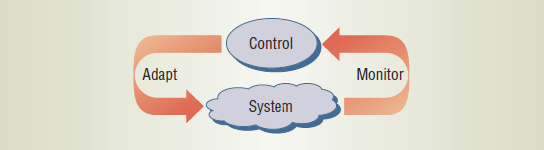
\includegraphics{images/selfhealing-closed-loop.png}
			\caption{Bucle cerrado}
			\label{fig:selfhealing-closed-loop}
		\end{figure}

		Otro sub proyecto del proyecto ABLE, denominado \textbf{Rainbow} (sobre el cual profundizaremos m�s adelante) utiliza
		esta t�cnica de \emph{closed-loop} para monitorear y reparar sistemas.

	\subsection{Lenguajes de Descripci�n de Arquitecturas}

		Un problema fundamental en el dise�o de arquitecturas de sistemas utilizando el estilo de componentes y
		conectores ha sido encontrar la notaci�n apropiada para definir dichas arquitecturas.

		Un buen lenguaje para describir arquitecturas deber�a permitir generar una documentaci�n clara sobre los componentes
		de la arquitectura, que luego servir� como base a los de\-sa\-rro\-lla\-do\-res, permitiendo a su vez razonar sobre
		las propiedades del sistema y automatizar su an�lisis, hasta pudiendo quiz�s llegar a utilizarse para la generaci�n
		autom�tica de parte del c�digo que implementar� la arquitectura. Tambi�n deber�a ser efectivo para poder validar de
		manera temprana decisiones arquitect�nicas, reduciendo as� el tiempo de implementaci�n y evitando utilizar
		ineficientemente recursos en el desarrollo del sistema.

		Una forma de describir dichas arquitecturas es mediante el modelado de objetos con UML, si bien este m�todo ha
		sido ampliamente aceptado y utilizado en la industria, tiene varios inconvenientes: el m�s importante e
		invalidante es que no provee un soporte directo para describir propiedades no funcionales. �sto hace dificultoso
		razonar sobre propiedades cr�ticas del sistema, como por ejemplo la \emph{performance} o la confiabilidad. �sta es la
		raz�n principal que ha motivado el avance de los ADLs (\emph{Architecture Description Languages}). Para m�s
		informaci�n sobre la discusi�n ADL's vs. UML, remitirse a \cite{ADLsVsUML}.

		La descripci�n de arquitecturas de sistemas basada en ADLs ha avanzado considerablemente en las �ltimas dos d�cadas,
		al punto de que ya permiten definir una base formal para su descripci�n y an�lisis.

	\subsubsection{Acme}
	\label{sec:acme}

		Acme\cite{ACME} es uno de los ADLs m�s reconocidos y utilizados, ha sido desarrollado en la universidad de Carnegie
		Mellon, m�s precisamente por el proyecto ABLE, liderado por el Dr. David Garlan.

		Acme es un pilar fundamental dentro del proyecto ABLE, ya que todo el proyecto gira en torno a la arquitectura de
		software de los sistemas, y es Acme quien permite describir formalmente dichas arquitecturas, por lo tanto todos los
		restantes sub proyectos utilizan Acme en menor o mayor medida.

		Adem�s de los beneficios de todo ADL, el lenguaje Acme y su kit de herramientas \emph{AcmeLib (Acme Tool Developer's
		Library)} proveen las siguientes capacidades fundamentales:

		\begin{itemize}
			\item Intercambio Arquitectural: al proveer un formato de intercambio gen�rico para dise�ar arquitecturas de
			software, Acme permite a los desarrolladores de herramientas de este tipo \footnote{Ejemplos de herramientas de
			descripci�n de arquitecturas y modelado UML podr�an ser: Enterprise Architect (\url{http://www.sparxsystems.com.au/})
			o Poseid�n (\url{http://www.gentleware.com/}), entre tantas otras.} integrar f�cilmente con otras herramientas
			complementarias. De esta manera, los arquitectos que usan herramientas basadas en Acme tienen un espectro m�s amplio
			de herramientas de	an�lisis y dise�o que quienes dise�an sus arquitecturas usando otros ADLs.
			\item Extensibilidad: Acme provee una base s�lida, gen�rica y extensible, y una infraestructura que evita que los
			desarrolladores vuelvan a construir herramientas de base. M�s a�n, debido a su idea originaria de lenguaje de
			intercambio gen�rico, Acme permite que las herramientas que se han desarrollado utiliz�ndolo sean compatibles con una
			gran variedad ADLs existentes y con herramientas con un m�nimo esfuerzo, y hasta en algunos casos sin esfuerzo alguno.
		\end{itemize}

		Actualmente, el lenguaje Acme y \emph{Acme Tool Developer's Library (AcmeLib)}, proveen una infraestructura gen�rica y
		extensible para describir, representar, analizar y generar descripciones de arquitecturas de software.

		A continuaci�n, observamos un breve ejemplo de una arquitectura modelada en el lenguaje ACME, la cual posee un
		sistema que contiene:
		\begin{itemize}
			\item un servidor HTTP, con algunas propiedades como por ejemplo fidelidad del contenido que provee.
			\item un cliente HTTP, tambi�n con algunas propiedades particulares como el tiempo de respuesta experimentado por el
			usuario.
		\end{itemize}

		\begin{Verbatim}[gobble=3]
			System system : ClientServerType = {
			    Component server : ServerT = new ServerT extended with {
			        Port http0 : HttpPortT;
			        Property cost;
			        Property fidelity;
			        Property load;
			    }
			    Component client : ClientT = new ClientT extended with {
			        Port p0 : HttpReqPortT = new HttpReqPortT extended with {
			            Property isArchEnabled = true;
			        }
			        Property deploymentLocation = "127.0.0.1";
			        Property isArchEnabled = true;
			        Property experRespTime;
			    }
			}
		\end{Verbatim}

		M�s adelante, en la secci�n \ref{sec:casosPracticos}, veremos otro ejemplo (m�s extenso) del lenguaje al mostrar la
		descripci�n completa en Acme de la arquitectura del sistema que utilizaremos para mostrar los resultados de la extensi�n
		implementada en el presente trabajo.

		\subsubsection{T�cticas y Estrategias}
		\label{sec:tacticasEstrategias}

			Hemos mencionado anteriormente que el objetivo de la auto reparaci�n es el alcanzar determinados atributos de
			calidad definidos para un determinado sistema, ajustando su comportamiento, de ser necesario, de acuerdo a
			las condiciones de ejecuci�n del mismo. En el libro \textbf{Software Architecture in Practice} \cite{BassClementz},
			Bass, Clements y Kazman caracterizan y formalizan dos herramientas que vienen siendo ampliamente utilizadas desde
			hace tiempo por los arquitectos de software en la industria, estas son: las \textbf{t�cticas} y las
			\textbf{estrategias}.

			Las \textbf{t�cticas} se definen como decisiones de dise�o tendientes a controlar las respuestas del sistema a
			determinados est�mulos, a fin de satisfacer uno o m�s atributos de calidad requeridos. La figura
			\ref{fig:tactics_control_to_response} muestra gr�ficamente el concepto de t�ctica arquitectural.

			\begin{figure}[h]
				\centering
					
\includegraphics{images/tactics_control_to_response.png}
				\caption{Visi�n gr�fica del concepto de t�ctica}
				\label{fig:tactics_control_to_response}
			\end{figure}

			Cada t�ctica es una opci�n de dise�o para el arquitecto, un ejemplo concreto podr�a ser el introducir redundancia en
			determinados componentes de la arquitectura (e.g. base de datos, servidores web replicados, etc.) para incrementar la
			dis\-po\-ni\-bi\-li\-dad del sistema.

			Por otro lado, una \textbf{estrategia} puede ser entendida como un procedimiento delineado por los arquitectos de
			\emph{software} para intentar llevar al sistema a un nivel d�nde los atributos de calidad se cumplan en el nivel
			deseado; haciendo uso de una o m�s t�cticas. Cada t�ctica es ejecutada �nicamente cuando el estado del sistema
			satisface las condiciones impuestas por la estrategia para dicha ejecuci�n. Por ejemplo, en una arquitectura
			cliente-servidor y al verse el tiempo de respuesta comprometido, una estrategia podr�a intentar agregar servidores
			mientras existan disponibles o, hasta que el tiempo de respuesta haya descendido por debajo de un determinado umbral.
			Esta l�gica ser�a descrita en la estrategia, mientras que ser� la t�ctica \verb@levantar-servidor@ la responsable de
			ejecutar la acci�n propiamente dicha. Notar que si bien esta estrategia est� dise�ada para mejorar el tiempo de
			respuesta, tambi�n afecta negativamente al \emph{concern} ``cantidad de servidores'' (correspondiente al atributo de
			calidad ``costo'') puesto que usualmente el utilizar mayor cantidad de servidores suele tener un costo econ�mico no
			despreciable.
			
			Cuando una estrategia se dise�a para mejorar un atributo de calidad en particular, se puede decir que los
			\emph{stakeholders} que definen dichos atributos de calidad obtienen cierto ``beneficio'' de las estrategias. Cada
			estrategia provee un nivel espec�fico de dicho beneficio, pero en contrapartida presenta un costo en tiempo y, sobre
			todo, en dinero. Es por este motivo que los \emph{stakeholders} deben participar en el proceso de decisi�n de c�ales
			estrategias se emplear�n para satisfacer los atributos de calidad definidos para el sistema. Ellos deber�n evaluar el
			retorno de la inversi�n (la relaci�n costo-beneficio) de aplicar cada estrategia para elegir la m�s conveniente.

			La estrategia es la herramienta propuesta por Rainbow para quitar al sistema de un estado no deseado.

	\subsection{Rainbow}

		\subsubsection{Introducci�n a Rainbow}

			La herramienta Rainbow, tambi�n dentro del marco del proyecto ABLE, tiene como finalidad permitir reducir el costo e
			incrementar la confiabilidad al realizar cambios en sistemas complejos de software, para esto Rainbow automatiza la
			adaptaci�n de sistemas de software a traves de sus modelos de arquitectura, tal cual fue descrito en la secci�n
			\ref{sec:ARSBMA}.

			Si bien en principio el enfoque de auto adaptaci�n basado en arquitecturas es atractivo, el mismo supone un n�mero
			significativo de desaf�os en el campo de la investigaci�n as� tambi�n como en el de la ingenier�a:

			\begin{itemize}
				\item En primer lugar, uno de los aspectos claves que Rainbow intenta cubrir es la habilidad de manejar una amplia
				variedad de sistemas con arquitecturas, propiedades de inter�s y mecanismos que soporten modificaciones din�micas
				completamente diferentes.

				\item Por otro lado, Rainbow intenta ser una soluci�n que permita reducir el costo de agregar control externo al
				sistema a reparar, puesto que crear los me\-ca\-nis\-mos de monitoreo y detecci�n de
				problemas desde cero para un sistema nuevo ser�a prohibitivamente costoso. El enfocar la auto reparaci�n de un
				sistema en su arquitectura permite disponer de una infraestructura reutilizable junto con mecanismos para adaptar
				dicha infraestructura a las necesidades espec�ficas de cada sistema.
			\end{itemize}

			Cabe mencionar que el caracter externo y no intrusivo de Rainbow representa una ventaja tambi�n cuando se
			desea implementar auto reparaci�n en sistemas cuyo c�digo fuente no est� disponible o no es plausible de ser
			modificado.

			\subsubsection{Arquitectura de Rainbow}

				La Figura \ref{fig:Rainbow_Framework} muestra la arquitectura de Rainbow. En resumidas palabras, el \emph{framework}
				utiliza un modelo arquitectural abstracto para monitorear las propiedades en \emph{runtime} del sistema que est�
				siendo ejecutado, eval�a el modelo para detectar violaciones a restricciones impuestas sobre el mismo y lleva a cabo
				adaptaciones en el sistema tendientes a eliminar tales violaciones.

				\begin{figure}[H]
					\centering
						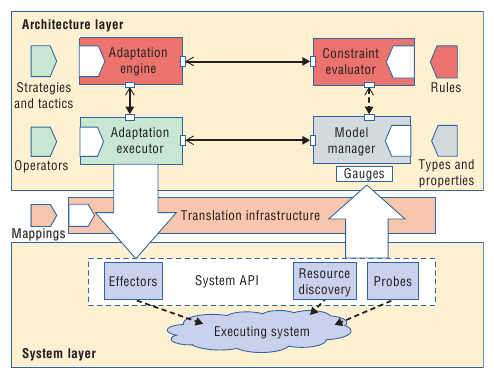
\includegraphics{images/Rainbow_Framework.png}
					\caption{Arquitectura de Rainbow}
					\label{fig:Rainbow_Framework}
				\end{figure}

				La infraestructura de adaptaci�n de Rainbow se divide en capas que proveen funcionalidades comunes a distintos
				sistemas auto adaptables logrando por lo tanto el objetivo de disponer de componentes reutilizables, a saber:
				\begin{enumerate}
					\item \textbf{Capa de Sistema}:\\
					En esta capa se define e implementa una interfaz de acceso al sistema que est� siendo ejecutado. Se define un
					mecanismo para medir variables de inter�s, materializado en \emph{Probes}: componentes que observan
					y miden diversos estados del sistema, para luego publicarlos.

					Adicionalmente, existe un mecanismo para descubrir recursos que puede ser utilizado especificando el tipo de
					recurso, entre otros criterios. Finalmente, los denominados \emph{Effectors} llevan a cabo las modificaciones
					propiamente dichas sobre el sistema.
					\item \textbf{Capa de Arquitectura}:\\
					En esta capa, los denominados \emph{Gauges} agregan informaci�n provenientes de los \emph{Probes} y
					mantienen constantemente actualizadas las propiedades correspondientes en el modelo arquitectural del sistema
					(descrito en ACME), el cual es manejado y accedido mediante un componente denominado \emph{Model Manager}. El
					\emph{Constraint Evaluator} chequea el modelo peri�dicamente y dispara la adaptaci�n en el caso que ocurra una
					violaci�n en alguna restricci�n impuesta sobre el modelo. En ese caso, el motor de adaptaci�n (\emph{Adaptation
					Engine}) determina el curso de acci�n y lleva a cabo la adaptaci�n necesaria.
					\item \textbf{Capa de Traducci�n}:\\
					Esta capa es la encargada de cubrir la brecha de abstracci�n existente entre el sistema en ejecuci�n y el modelo
					de su arquitectura (en ambos sentidos). En esta infraestructura, un repositorio de traducci�n mantiene diversos
					mapeos compartidos por distintos componentes dentro de esta capa, por ejemplo, una operaci�n a nivel modelo de la
					arquitectura en su correspondiente operaci�n de \emph{runtime}:

					\begin{Verbatim}[gobble=7]
						       Componente de Log::desactivar       <==>       Logger.disableLog()
					\end{Verbatim}
				\end{enumerate}

				Rainbow es un \emph{framework} desarrollado en el lenguaje de programaci�n Java\textsuperscript{\texttrademark} y
				todos los derechos sobre el c�digo fuente pertenecen al grupo ABLE de la Universidad de Carnegie Mellon. Los autores
				de este trabajo solicitaron permiso a este grupo para poder acceder al c�digo fuente de Rainbow para poder realizar
				la extensi�n objeto de este trabajo. En la wiki oficial de Rainbow pueden encontrarse instrucciones para
				instalar versiones ya compiladas del \emph{framework}. Para m�s informaci�n, visitar
				\url{http://rainbow.self-adapt.org/RainbowInstall}.

		\subsubsection{Conocimiento espec�fico del sistema}
		
			En la secci�n anterior hemos descrito la infraestructura b�sica provista por Rainbow. Es de notar que la misma no es
			suficiente para satisfacer las necesidades puntuales de auto adaptaci�n de un sistema en particular. Para
			lograr esto, es necesario extender dicha infraestructura, agregando conocimiento espec�fico del sistema que se desea
			adaptar. Este conocimiento (t�picamente no reutilizable entre distintos sistemas) incluye el modelo operacional
			del sistema, que define par�metros como tipos de componentes y propiedades, restricciones de comportamiento,
			estrategias de adaptaci�n, interfaz para acceder a la informaci�n de \emph{runtime} del sistema, as� tambi�n como
			para hacer efectivas las estrategias de reparaci�n, etc.

		\subsubsection{Stitch}

			A fin de disponer de una forma suficientemente expresiva de definir t�cticas y estrategias, Rainbow incluye
			un lenguaje de \emph{scripting} de prop�sito espec�fico llamado \textbf{Stitch}, el cual permite plasmar el
			conocimiento rutinario de las personas sobre adaptaci�n de sistemas de software.

			Algunas de las caracter�sticas innovadoras de Stitch:
			\begin{itemize}
				\item \textbf{Control del sistema}: La selecci�n de la pr�xima acci�n a ejecutar en el contexto de una estrategia
				depende de los efectos observados luego de la acci�n previa.
				\item \textbf{Sensibilidad al contexto}: La selecci�n de la mejor estrategia se realiza considerando el estado
				actual del sistema, mediante la inspecci�n de algunas de sus propiedades.
				\item \textbf{Asincronismo}: Stitch permite especificar un tiempo de demora luego de la ejecuci�n de una t�ctica
				para que los efectos de la t�ctica se puedan ver reflejados en el sistema.
			\end{itemize}

		\subsubsection{Ejemplo de una T�ctica en Stitch}

			En la figura \ref{fig:tactics_example} se puede apreciar un ejemplo de una t�ctica definida en Stitch para ser
			utilizada por Rainbow. Primeramente, se importa el modelo de la arquitectura del sistema en cuesti�n junto con la
			implementaci�n de un operador que permite impactar al sistema en ejecuci�n (estos operadores suelen ser provistos por
			el usuario de la aplicaci�n).
			
			\begin{figure}[h]
				\centering
					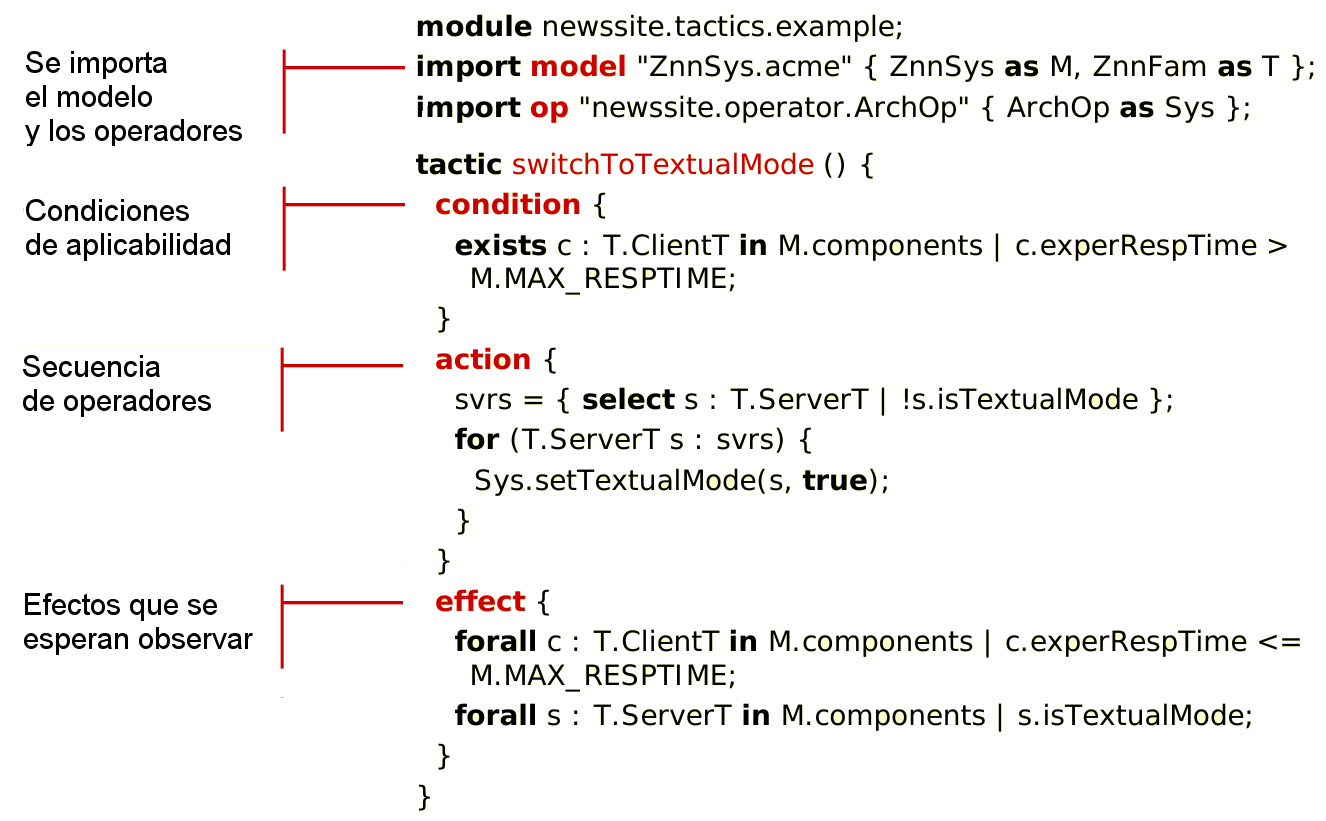
\includegraphics[width=0.98\textwidth]{images/tactics_example.png}
				\caption{Ejemplo de una t�ctica en Stitch}
				\label{fig:tactics_example}
			\end{figure}
			
			La t�ctica consiste en disminuir la fidelidad (a modo s�lo texto) del contenido provisto por todos los servidores
			cuando se detecta que al menos un cliente experimenta un tiempo de respuesta superior a un determinado umbral. Para lograr
			esto, Rainbow inspecciona las propiedades del modelo de la arquitectura del sistema, definido en ACME, el c�al se
			supone constantemente actualizado por Rainbow con respecto al estado actual del sistema en ejecuci�n.
			
			Por �ltimo, se especifica que el efecto esperado de ejecutar la t�ctica consiste en que todos los clientes
			experimenten un tiempo de respuesta inferior al umbral y que, por otro lado, todos los servidores se encuentren
			prestando servicio en modo s�lo texto.

		\subsubsection{Ejemplo de una Estrategia en Stitch}

			En la figura \ref{fig:strategies_example} podemos ver un ejemplo de una estrategia definida en Stitch para ser
			utilizada por Rainbow.

			\begin{figure}[h]
				\centering
					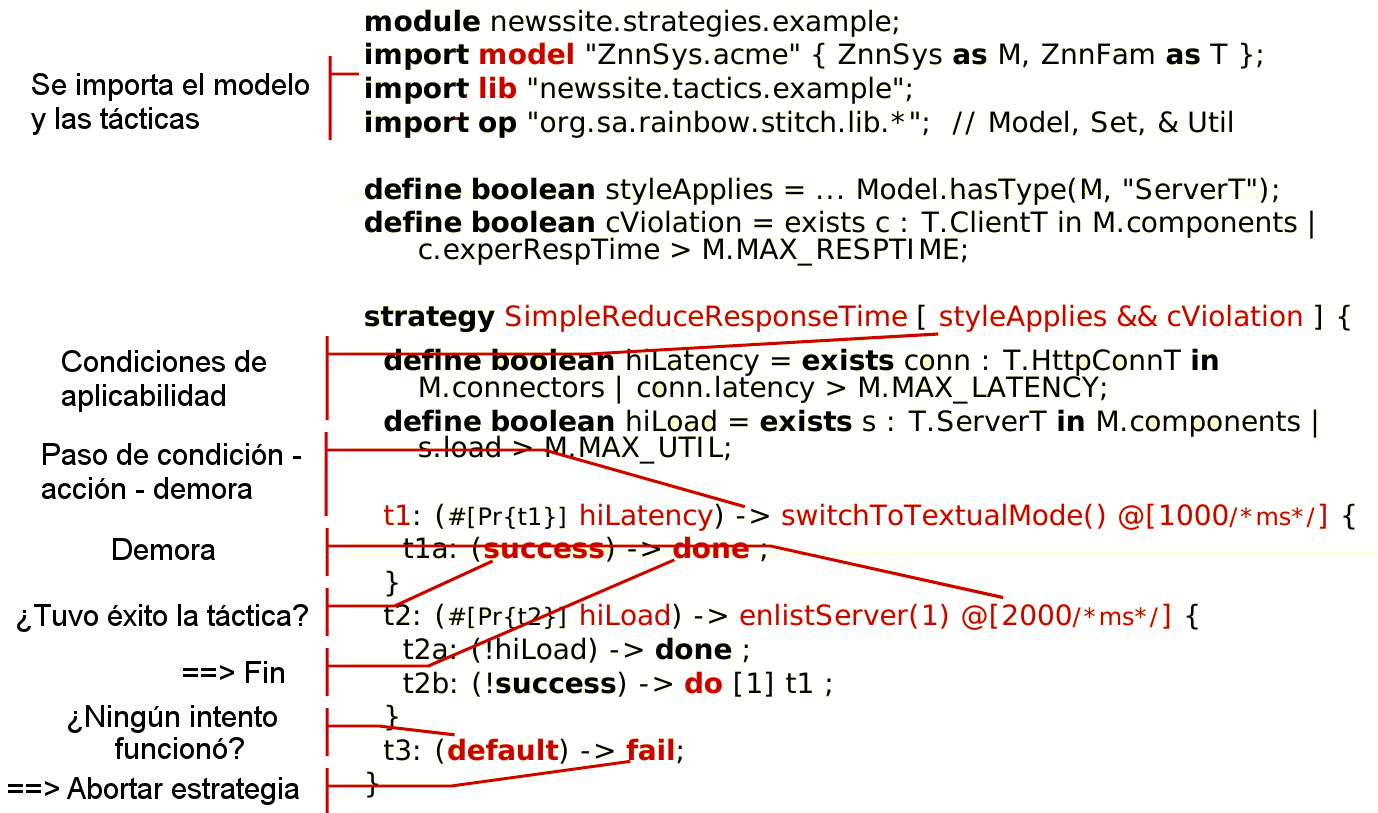
\includegraphics[width=0.98\textwidth]{images/strategies_example.png}
				\caption{Ejemplo de una estrategia en Stitch}
				\label{fig:strategies_example}
			\end{figure}

			La estrategia representa un algoritmo simple para disminuir el tiempo de respuesta experimentado por el usuario de un
			sistema cliente-servidor. Se definen algunos predicados de primer orden que predican sobre propiedades del modelo de
			la arquitectura del sistema, el cual se presume constantemente actualizado por Rainbow con respecto al sistema en
			ejecuci�n.
			
			El primer paso de la estrategia consiste en verificar que haya en la arquitectura un conector que presente
			alta latencia, en ese caso, se invoca la t�ctica definida en la Figura \ref{fig:tactics_example}, la cual cambia la
			fidelidad de todos los servidores a modo s�lo texto, y se espera 1 segundo antes de determinar el �xito o no de la
			ejecuci�n de la t�ctica. Si la t�ctica tuvo �xito, la estrategia finaliza satisfactoriamente. Sino, la estrategia
			chequea la existencia de al menos un servidor con alta carga, y en caso afirmativo, ejecuta otra t�ctica que consiste
			en agregar un servidor m�s en pos de mejorar el \emph{concern} tiempo de respuesta. Si luego de esperar 2 segundos
			para que los efectos de la t�ctica puedan verse reflejados en el sistema, todos los servidores operan con carga
			normal, la estrategia finaliza exitosamente, caso contrario, la misma se considera fallida.

		\subsubsection{\emph{Exponential Moving Average}}
		\label{sec:exponentialAverage}

			El proceso de adaptar un sistema de manera din�mica puede llegar a ser muy costoso, por ejemplo, en un sistema
			cliente-servidor, el asignar m�s servidores para atender las peticiones de los usuarios implica normalmente un coste
			monetario no despreciable. Otro ejemplo podr�a ser el suspender temporalmente la reproducci�n de videos en un sitio
			de noticias. Si bien esta decisi�n puede servir para disminuir el tiempo de respuesta experimentado por los usuarios
			en un contexto de alta carga, tambi�n provoca una clara disminuci�n en la calidad del servicio ofrecido. Estos
			ejemplos concretos sirven para inferir que el disparar un mecanismo de auto reparaci�n en un sistema debe ser una
			decisi�n tomada con cierta cautela y en base a datos confiables y sostenidos en el tiempo.
			
			Hemos visto anteriormente, de manera somera, de que forma Rainbow (mediante estrategias y t�cticas definidas en el
			lenguaje Stitch) utiliza datos sobre el sistema en ejecuci�n para decidir el mejor camino a tomar para adaptar el
			sistema. Consideremos un escenario donde una estrategia debe decidir si el �ltimo paso ejecutado fue exitoso o no.
			Para eso, deber� consultar una o m�s propiedades del sistema en ejecuci�n, las cuales podr�an llegar a no ser
			representativas del entorno \emph{real} en que el sistema se encuentra, debido a la presencia de (\emph{outliers}),
			i.e. valores aislados considerablemente distintos al resto de los datos recientes que se usan para tomar
			decisiones.
			
			Rainbow implementa un mecanismo que permite evitar accionamientos prematuros de la auto reparaci�n debido a la
			presencia de \emph{outliers}. El mentado mecanismo utiliza \emph{Exponential Moving Average}\footnote{Para
			m�s informaci�n, visitar \url{http://en.wikipedia.org/wiki/Exponential_moving_average}}, que permite ponderar los
			valores hist�ricos de la(s) propiedad(es) del sistema que se consultan para tomar decisiones. La funci�n de suavizado
			que implementa esta heur�stica se define inductivamente de la siguiente manera:

			\begin{equation}
				S_0 = Y_0
			\end{equation}
			\begin{equation}
				S_t = \alpha \times Y_t + (1-\alpha) \times S_{t-1}
			\end{equation}

			donde $\alpha$ se denomina \textbf{factor de suavizado} y $0 < \alpha < 1$.
			
			El valor suavizado $S_t$ no es ni m�s ni menos que un promedio ponderado de la �ltima observaci�n $Y_t$ y el valor
			suavizado previo $S_{t-1}$.
			
			Notar que con valores \emph{altos} de $\alpha$, el �ltimo valor observado tendr� m�s preponderancia que el valor
			hist�rico (suavizado) anterior. Por el contrario, con un $\alpha$ tendiendo a cero, la �ltima observaci�n de una
			propiedad de la arquitectura pr�cticamente no tendr� relevancia sobre el valor promedio $S_t$.
			
			No existe un procedimiento formal para determinar el valor de $\alpha$, en el caso particular de las pruebas
			realizadas en este trabajo, se ha elegido $\alpha = 0.3$, es decir que, se ponderar� con un 30\% al �ltimo valor
			observado mientras que el valor hist�rico tendr� un peso del 70\%; con esto nos aseguramos que los valores de las
			propiedades del sistema que son relevantes para la auto adaptaci�n no fluct�en bruscamente debido a unos pocos
			\emph{outliers}.

	\subsubsection{Znn}

		Znn es un sistema que simula un sitio web de noticias, el cual naci� en el contexto de la tesis de doctorado
		\cite{TesisOwen} de Shang-Wen Cheng, un investigador de la universidad de Carnegie Mellon. En dicha tesis, se eval�a a
		Rainbow en los siguientes aspectos:
		\begin{itemize}
			\item su efectividad para mantener los atributos de calidad ante condiciones cambiantes.
			\item la sobrecarga de procesamiento que implica la auto reparaci�n.
			\item el esfuerzo que implica agregar auto reparaci�n a Znn mediante Rainbow.
		\end{itemize}

		Si bien Znn y sus herramientas asociadas (\emph{probes}, \emph{gauges}, t�cticas, estrategias, etc.) nacieron con
		el �nico objetivo de evaluar la efectividad de Rainbow, las mismas han sido abiertas a la comunidad para que puedan
		ser utilizadas para tomar m�tricas y poder comparar distintos \emph{frameworks} de auto reparaci�n.

		Znn provee un entorno de simulaci�n de una arquitectura cliente-servidor ampliamente configurable que permite
		representar situaciones espec�ficas de ejecuci�n y controlar las variables de simulaci�n permitiendo modificarlas en
		cualquier punto.
		
		Por ejemplo, es posible configurar a Znn para que inicie con solamente 2 clientes, mostrando all� un desempe�o
		aceptable y que luego se agreguen 10 clientes, comprometiendo as� la \emph{performance} del sistema. De esta
		manera, Znn permite simular c�mo responder�an las estrategias implementadas ante dicha situaci�n.

		Rainbow soporta dos modos de ejecuci�n: el \textbf{modo normal}, donde el \emph{framework} se conecta con un sistema
		real, y un \textbf{modo simulaci�n}, el cual permite probar las herramientas de auto reparaci�n implementadas por los
		usuarios sin necesidad de conectar a Rainbow con un sistema real en ejecuci�n.
		
		En el presente trabajo se utilizar� el modo simulaci�n para los casos de prueba, tomando las estrategias y t�cticas
		provistas por Znn. �stas debieron ser adaptadas para que puedan seguir funcionando con los cambios propuestos en el
		presente trabajo.

	\subsection{Escenarios de Atributos de Calidad}
	\label{sec:QAS}

		Un escenario de atributos de calidad (de ahora en m�s, simplemente ``escenario'') es la especificaci�n de un
		requerimiento para un atributo de calidad en particular. Consiste de seis partes:

		\begin{itemize}
			\item \textbf{Fuente del est�mulo}: Es una entidad (un ser humano, otro sistema o cualquier otro actor) que gener� el
			est�mulo.
			\item \textbf{Est�mulo}: la condici�n que debe ser tenida en cuenta cuando llega al sistema.
			\item \textbf{Entorno}: el est�mulo ocurre bajo ciertas condiciones, e.g. entorno de alta carga, entorno normal,
			sistema no funcionando, etc.
			\item \textbf{Artefacto}: el sistema o partes de �l afectadas por el est�mulo.
			\item \textbf{Respuesta}: refiere a qu� hace el sistema ante la llegada del est�mulo.
			\item \textbf{Medici�n de la respuesta}: cuando ocurre la respuesta, debe ser medible de alguna manera para que el
			requerimiento pueda ser \emph{testeado}.
		\end{itemize}

		\begin{figure}[h]
			\centering
				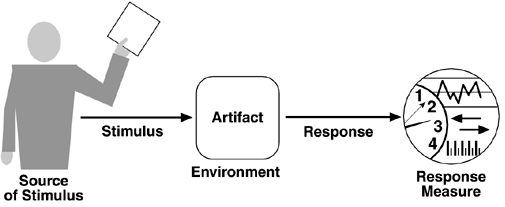
\includegraphics{images/scenario.png}
			\caption{Visi�n gr�fica de un escenario}
			\label{fig:scenario}
		\end{figure}

		Los escenarios son peque�as historias que describen una interacci�n con el sistema, la cual impacta sobre un atributo
		de calidad en particular. Por ejemplo, un escenario sobre disponibilidad podr�a ser:
		\begin{quote}
		``Un proceso del sistema recibe un mensaje externo no anticipado durante un modo de operaci�n normal. El proceso
		informa al operador sobre la recepci�n del mensaje y contin�a su operaci�n sin ca�das.''
		\end{quote}

		\begin{figure}[ht]
			\centering
				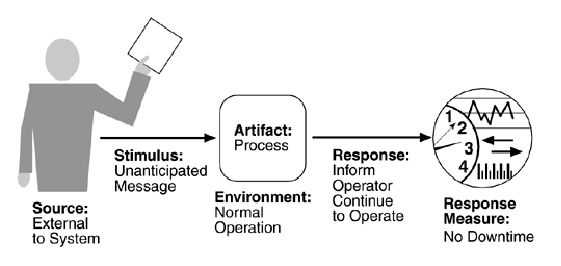
\includegraphics{images/scenario_availability_example.png}
			\caption{Ejemplo de un escenario de disponibilidad}
			\label{fig:scenario_availability_example}
		\end{figure}

		Este escenario se descompone de la siguiente manera:
		\begin{itemize}
			\item \textbf{Fuente del est�mulo}: Cualquier fuente externa
			\item \textbf{Est�mulo}: Mensaje no anticipado
			\item \textbf{Entorno}: Operaci�n normal
			\item \textbf{Artefacto}: Proceso interno
			\item \textbf{Respuesta}: Informar al operador y seguir operando
			\item \textbf{Medici�n de la respuesta}: sin ca�das (\emph{downtime})
		\end{itemize}

		Los escenarios permiten obtener el punto de vista de un grupo diverso de \emph{stakeholders} (arquitectos,
		desarrolladores, usuarios, el \emph{sponsor}, etc). Estos escenarios pueden luego ser utilizados para analizar y
		definir la arquitectura del sistema e identificar \emph{concerns} y posibles estrategias para atacar problemas.

		\subsubsection{QAW}
			Existe una metodolog�a definida por el Software Engineering Institute (SEI) conocida como \textbf{Quality Attribute
			Workshops (QAW)}, cuya principal herramienta son los escenarios. Los QAW proveen un m�todo para identificar los
			atributos de calidad cr�ticos de la arquitectura de un sistema, tales como disponibilidad, \emph{performance},
			seguridad, etc, que son derivados de objetivos del negocio. QAW no presupone la existencia de una arquitectura del
			sistema, sino que fue desarrollado como consecuencia de la necesidad de \emph{stakeholders} y arquitectos de un
			m�todo que permita identificar los atributos de calidad importantes para el correcto funcionamiento del sistema
			\textbf{antes de definir su arquitectura}.
	
			Los QAW son reuniones en las que participan todos los \emph{stakeholders}, en las que se definen los escenarios que
			en definitiva representar�n los requerimientos de atributos de calidad que el sistema idealmente deber� satisfacer.
			Una vez definidos todos los escenarios, el siguiente paso del QAW consiste en priorizarlos y refinarlos,
			especificando claramente todos las partes que los componen y determinando el atributo de calidad asociado a cada
			escenario. El proceso de refinar los escenarios permite a los \emph{stakeholders} comunicarse entre ellos, exponiendo
			supuestos que pueden no ser tan claros para el resto de los participantes, y proporcionando una visi�n de c�mo
			interact�an los atributos de calidad entre s�, sirviendo de base para definir \emph{tradeoffs} entre estos atributos.
	
			El proceso QAW termina con la lista de escenarios refinados y priorizados. Los mismos pueden servir para definir casos
			de pruebas, o como semillas para el proceso ATAM, sobre el cual discutiremos en la siguiente secci�n.

			Si bien no es condici�n necesaria para poder usar Arco Iris, el utilizar la metodolog�a QAW, tal cual est�
			descrita en \cite{QAW}, es recomendado ya que Arco Iris har� uso intensivo de los escenarios de atributos de calidad
			y, por lo tanto, de su correcta definici�n depender� el nivel de optimizaci�n y flexibilizaci�n que la extensi�n a
			Rainbow pueda alcanzar al auto reparar un sistema de \emph{software}.

	\subsection{ATAM}
	\label{sec:atam}

		\subsubsection{Terminolog�a necesaria}

			Antes de profundizar sobre ATAM, es necesario clarificar ciertos t�rminos que ser�n utilizados en el desarrollo de la
			presente secci�n. Estos t�rminos son:
			
			\begin{itemize}
				\item \textbf{Riesgo}: decisi�n arquitect�nica potencialmente problem�tica.
				\item \textbf{Punto sensible}: propiedad de uno o m�s componentes (y/o relaciones entre componentes) que es cr�tica
				para poder alcanzar un atributo de calidad determinado. Por ejemplo, un m�dulo de cifrado es un punto sensible para
				el atributo de calidad ``seguridad''.
				\item \textbf{Punto de \emph{tradeoff}}: se trata de un componente de la arquitectura donde se afecta m�s
				de un atributo de calidad (y por ende, tambi�n es un punto sensible para dichos atributos de calidad). Por ejemplo,
				el m�dulo de cifrado mencionado anteriormente ser�a un punto de \emph{tradeoff} de haber requerimientos de
				\emph{performance}, ya que afecta positivamente la seguridad y negativamente la \emph{performance} del sistema. 
				\item \textbf{\emph{Non risks}} son buenas decisiones de arquitectura que normalmente est�n impl�citas en la
				arquitectura.
			\end{itemize}

		\subsubsection{Analizando arquitecturas con ATAM}

			El m�todo para el an�lisis de \emph{tradeoffs} o, de sus siglas en ingl�s, ATAM (Architecture Tradeoff Analysis
			Method)\cite{ATAM}, al igual que QAW, ha sido desarrollado por el SEI y es una t�cnica que permite analizar
			arquitecturas de \emph{software} con el objetivo de validar requerimientos de atributos de calidad, su interacci�n
			(conocidos como \emph{tradeoffs}), detectar problemas de manera temprana e identificar riesgos y puntos sensibles.
			
			Usualmente, las arquitecturas de \emph{software} son complejas, e involucran muchos \emph{tradeoffs} de dise�o. Sin un
			proceso de an�lisis formal, no es posible garantizar que las decisiones de arquitectura	tomadas \textendash en
			particular aquellas que afectan al cumplimiento de requerimientos de calidad \textendash son adecuadas para mitigar
			los riesgos.
	
			La meta de evaluar una arquitectura con ATAM es entender las consecuencias de las decisiones arquitect�nicas con
			respecto a los requerimientos de atributos de calidad del sistema. Otro objetivo fundamental de ATAM es determinar si
			dichos requerimientos pueden ser alcanzados con la arquitectura concebida, antes de destinar grandes cantidades de
			recursos a la construcci�n del \emph{software}.
	
			ATAM es un m�todo estructurado y repetible, ayudando as� a plantear las preguntas correctas sobre la arquitectura
			de manera temprana en el proyecto, durante las etapas de an�lisis de requerimentos y de dise�o, en las
			cuales los problemas detectados pueden ser corregidos sin mayores costos. ATAM gu�a a los usuarios del m�todo
			(\emph{stakeholders}) para que busquen riesgos en la arquitectura y soluciones a dichos riesgos.
	
			Cabe mencionar que los QAW han surgido como consecuencia del uso de ATAM, puesto que era requerida una herramienta o
			m�todo que permitiera identificar los requerimientos de atributos de calidad m�s importantes del sistema,
			\textbf{antes de que existiese la arquitectura} sobre la cual ATAM trabajar�a. Luego de observar los pasos del
			m�todo ATAM que detallaremos a continuaci�n, no ser� dif�cil para el lector inferir que en realidad ATAM incluye una
			versi�n simplificada de QAW.
	
		\subsubsection{Pasos del m�todo ATAM}

			A continuaci�n se describen los pasos del m�todo ATAM:
	
			\noindent \underline{\emph{Presentaci�n}}

			\begin{enumerate}
				\item \textbf{Presentar ATAM.} El m�todo es descrito a los \emph{stakeholders}.
				\item \textbf{Presentar las metas del negocio.} El \emph{project manager} describe los objetivos del
				negocio que motivan el desarrollo.
				\item \textbf{Presentar la arquitectura.} El equipo de arquitectos presenta la arquitectura propuesta,
				haciendo foco en c�mo la misma satisface las metas del negocio.
			\suspend{enumerate}
			
			\noindent \underline{\emph{Investigaci�n y An�lisis}}
			
			\resume{enumerate}
				\item \textbf{Identificar enfoques arquitect�nicos.} Los enfoques arquitect�nicos son identificados
				por el equipo de arquitectura, pero no analizados.
				\item \label{arbolUtilidad} \textbf{Generar el �rbol de utilidad.} Se recaban los atributos de calidad que agregan
				utilidad al sistema y se los especifica en forma de escenarios priorizados.
				\item \label{enfoques} \textbf{Analizar enfoques arquitect�nicos.} Se delinean enfoques arquitect�nicos para los
				escenarios de mayor prioridad recabados en (\ref{arbolUtilidad}). Durante este paso, se identifican riesgos
				arquitect�nicos, puntos sensibles y puntos de \emph{tradeoff}.
			\suspend{enumerate}

			\noindent \underline{\emph{Testing}}

			\resume{enumerate}
				\item \label{brainstorming} \textbf{\emph{Brainstorming} y priorizaci�n de escenarios.} Basado en los escenarios del
				�rbol de utilidad, se genera un conjunto mayor de escenarios m�s espec�ficos. Estos nuevos escenarios son
				priorizados v�a un proceso de votaci�n.
				\item \textbf{Analizar enfoques arquitect�nicos.} Se reitera el paso (\ref{enfoques}) pero con los escenarios m�s
				prioritarios encontrados en el paso (\ref{brainstorming}), con el objetivo de encontrar nuevos riesgos, puntos
				sensibles y \emph{tradeoffs}.
			\suspend{enumerate}

			\noindent \underline{\emph{Reporting}}

			\resume{enumerate}
				\item \textbf{Presentar resultados.} Basado en toda la informaci�n recolectada durante el proceso (escenarios,
				el �rbol de utilidad, riesgos, puntos sensibles y puntos de \emph{tradeoff}), el equipo de ATAM escribe un reporte
				detallando esta informaci�n y las estrategias de mitigaci�n propuestas.
			\end{enumerate}

			\begin{figure}[h]
				\centering
					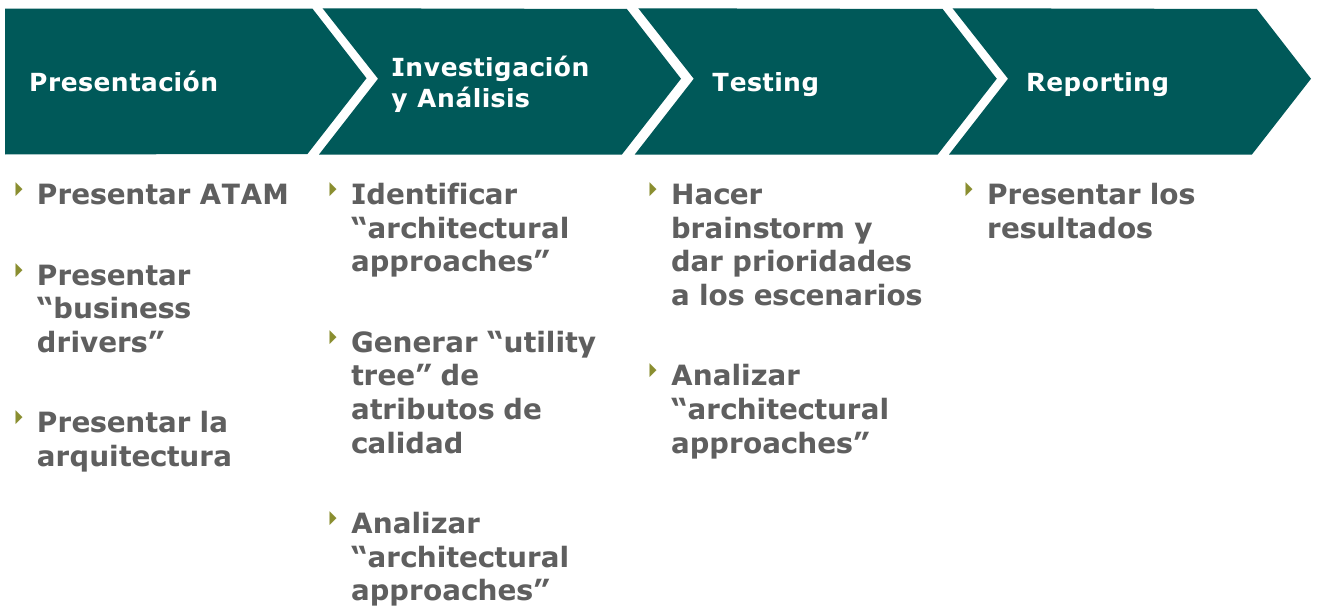
\includegraphics[width=0.85\textwidth]{images/ATAM_steps.png}
				\caption{Pasos de ATAM}
				\label{fig:ATAM_steps}
			\end{figure}

\newpage

\section{Extensi�n a Rainbow: Arco Iris}

	\subsection{Introducci�n}

		Como ya se ha comentado anteriormente, la idea de este trabajo es extender el \emph{framework} Rainbow para poder
		lograr un mecanismo de auto reparaci�n m�s flexible y con mayor capacidad expresiva, y con el objetivo de proveer visibilidad
		a los \emph{stakeholders} de la aplicaci�n sobre dicho proceso, permiti�ndoles involucrarse en la definici�n de
		escenarios de atributos de calidad del sistema, de sus prioridades relativas y de las estrategias a considerar en la
		auto reparaci�n del sistema cuando un escenario deja de cumplirse.

		A fin de lograr lo antedicho, se propone extender el \emph{framework} Rainbow, con la anuencia y apoyo de los
		integrantes del proyecto ABLE, quienes poseen su propiedad intelectual.

	\subsection{Rainbow \emph{out of the box}}

		En el diagrama de colaboraci�n de objetos que se muestra en la Figura \ref{fig:Rainbow_Architecture} se pueden 
		observar los principales componentes de la arquitectura de Rainbow.

		\afterpage{\clearpage
		\begin{figure}[H]
			\centering
				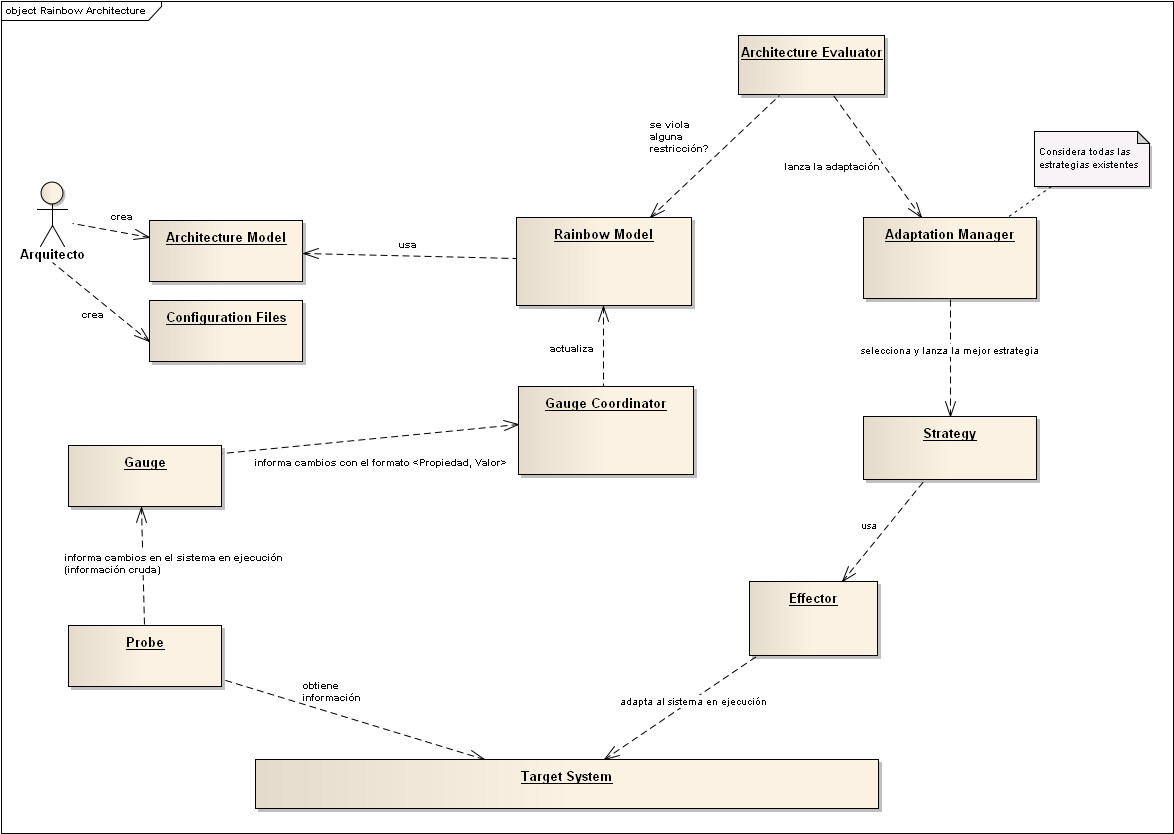
\includegraphics[width=1.00\textwidth]{images/Rainbow_Architecture.png}
			\caption{Arquitectura de Rainbow}
			\label{fig:Rainbow_Architecture}
		\end{figure}}
		
		Observamos que, en Rainbow, una persona con rol de arquitecto (o similar) es el encargado de configurar el 
		\emph{framework} utilizando, b�sicamente, dos v�as:
		\begin{enumerate}
			\item la creaci�n de un modelo de la arquitectura del sistema al cual Rainbow va a adaptar. Dicho modelo se
			especifica utilizando el estilo de componentes y conectores (C\&C) y el lenguaje de descripci�n de arquitecturas
			ACME (ver secci�n \ref{sec:acme}). En dicho lenguaje, los componentes y conectores poseen propiedades (con valores
			asociados), restricciones y tambi�n se ofrece la posibilidad de especificar invariantes a nivel de sistema o sub
			sistema. Dichos invariantes y restricciones ser�n evaluados peri�dicamente por Rainbow para verificar que el sistema
			funcione dentro de los l�mites determinados como normales.
			\item la generaci�n de un conjunto de archivos de configuraci�n que especifican diversos aspectos relacionados con
			la definici�n del sistema a auto reparar, como por ejemplo: ubicaci�n f�sica del archivo ACME que describe la
			arquitectura del sistema, archivos de t�cticas y estrategias de reparaci�n (escritos en \emph{Stitch}), datos para
			la configuraci�n de la conexi�n de Rainbow con el sistema en \emph{runtime}, etc.
		\end{enumerate}

		Podemos ver tambi�n en el gr�fico anterior que los denominados \emph{Probes} son los componentes designados para
		interactuar directamente con el sistema a adaptar (el \emph{Target System}), obteniendo as� informaci�n relevante a los
		fines de su auto reparaci�n. Dicha informaci�n no es interpretada dentro de los \emph{probes}, sino que ellos delegan
		dicha tarea a los denominados \emph{Gauges}. Estos componentes son los encargados de interpretar la informaci�n provista por
		los \emph{probes} y traducirla a pares \verb@<Propiedad,Valor>@ donde \verb@Propiedad@ refiere al nombre de una
		propiedad correspondiente a un componente o conector de la arquitectura del sistema a adaptar, mientras que
		\verb@Valor@ es el nuevo valor que poseer� dicha propiedad.

		Normalmente, por cada tipo relevante de \emph{concern} que interese ser monitoreado en tiempo de ejecuci�n existe un
		par \verb@<Gauge,Probe>@ asociado. Un ejemplo de \emph{concern} podr�a ser: ``tiempo de respuesta experimentado por el
		usuario'', el cual es un \emph{concern} relacionado al atributo de calidad \emph{performance}.

		El \emph{Gauge Coordinator}, tal como su nombre lo sugiere, coordina la informaci�n provista por todos los
		\emph{gauges} y se encarga de notificar los cambios en el sistema en ejecuci�n al componente \emph{Rainbow Model}.
	
		\emph{Rainbow Model}, componente clave en la arquitectura del \emph{framework}, tiene como principal responsabilidad
		hacer efectiva la actualizaci�n de los valores de la propiedades de los componentes, conectores, sub sistemas o
		sistemas del modelo de arquitectura de la aplicaci�n a adaptar. Tambi�n es quien tiene el conocimiento necesario para
		detectar violaciones a las restricciones e invariantes presentes en el modelo de arquitectura con el cual el
		\emph{framework} ha sido configurado.

		Por otra parte, existe otro componente llamado \emph{Architecture Evaluator}, el cual consulta peri�dicamente a
		\emph{Rainbow Model} para tomar conocimiento de violaciones a restricciones definidas en el modelo de la arquitectura.
		En el caso de existir alguna violaci�n, el \emph{Architecture Evaluator} dispara el mecanismo de adaptaci�n invocando
		al \emph{Adaptation Manager}.

		El \emph{Adaptation Manager}, uno de los componentes m�s importantes de Rainbow, sigue una l�gica un tanto compleja
		(explicada en detalle en la secci�n \ref{sec:strategySelection}) para determinar la estrategia de reparaci�n que deja
		al sistema en el mejor estado posible, para luego ejecutarla.
		
		La \emph{Estrategia} contiene la l�gica necesaria para reparar el sistema en ejecuci�n mediante el uso de
		\emph{T�cticas}, que a su vez, utilizan a los denominados \emph{Effectors}, los cuales son componentes que realizan
		acciones simples y concretas sobre el sistema en ejecuci�n, como por ejemplo ``aumentar el nivel de logging de un
		componente determinado''.

	\subsection{Rainbow + Escenarios = ``Arco Iris''}

			En el presente apartado se presenta someramente las caracter�sticas principales de la arquitectura de Rainbow
			luego de incorporar las extensiones planteadas en el presente trabajo, a las cuales denominamos ``Arco Iris''.

		\subsubsection{Arquitectura de Arco Iris}

			En la figura \ref{fig:Rainbow_Architecture_With_Scenarios} podemos observar como luce la arquitectura
			del \emph{framework} con la incorporaci�n de las extensiones realizadas.

			\afterpage{\clearpage
			\begin{figure}[H]
				\centering
				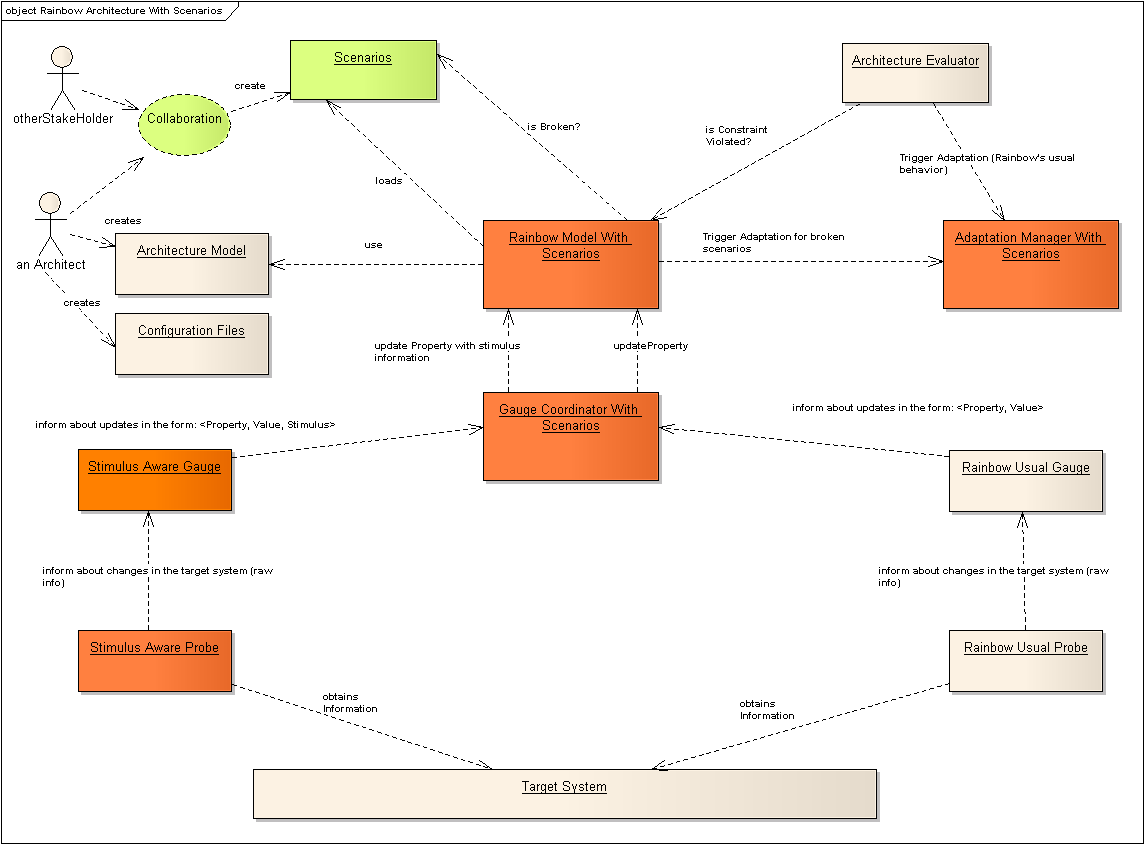
\includegraphics[width=1.00\textwidth]{images/Rainbow_Architecture_With_Scenarios.png}
				\caption{Arquitectura de Arco Iris}
				\label{fig:Rainbow_Architecture_With_Scenarios}
			\end{figure}}

			El arquitecto sigue realizando las mismas tareas que realizaba en Rainbow (i.e. ``alimentarlo'' con el
			modelo de la arquitectura del sistema a adaptar y con archivos de configuraci�n requeridos por Rainbow) pero ahora se
			le suma una tarea m�s: el configurar los escenarios de atributos de calidad; tarea que realiza en conjunto con una o
			m�s personas que asumen distintos roles que normalmente se engloban en la palabra \emph{stakeholders} (e.g. analistas
			funcionales, usuarios del sistema, l�deres, clientes, el \emph{sponsor} del proyecto, etc.)

			En la versi�n original de Rainbow (i.e. sin extensiones) el \emph{framework} deja al usuario (e.g. el arquitecto) la
			responsabilidad de codificar los \emph{probes} y \emph{gauges} que recolectar�n informaci�n del sistema a adaptar y
			traducir�n esa informaci�n a cambios en los valores de las propiedades del sistema. Esto sigue siendo igual en
			Rainbow con las extensiones provistas por Arco Iris, es decir, el usuario sigue siendo el encargado de crear los
			componentes que en tiempo de ejecuci�n encuestan al sistema peri�dicamente para obtener informaci�n relevante y
			mantener actualizado el modelo de la arquitectura subyacente.

			En el diagrama se puede observar que, en Arco Iris, tanto los \emph{probes} como los \emph{gauges} ahora poseen
			conocimiento del concepto de \textbf{est�mulo} (tal cual es descrito en los escenarios de atributos de calidad de ATAM).
			A diferencia de los utilizados en Rainbow, los \emph{probes} implementados para trabajar con Arco Iris deber�n
			indicar el est�mulo al cual est�n asociados, mientras que los \emph{gauges} deber�n interpretar esta informaci�n y
			notificar al \emph{Arco Iris Model} de la actualizaci�n sobre el modelo indicando el est�mulo desencadenante. Las
			novedades sobre los cambios ocurridos en el sistema en \emph{runtime} ser�n informados con el siguiente formato:
			\verb@<Propiedad,Valor,Est�mulo>@

			En funci�n de las modificaciones al modelo original de Rainbow descritas en el p�rrafo anterior, el componente
			\emph{Gauge Coordinator} ha sido extendido (i.e. \emph{Arco Iris Gauge Coordinator}) conservando el comportamiento
			original provisto por Rainbow. De esta manera, Arco Iris puede coordinar informaci�n proveniente de \emph{gauges} de
			Rainbow y/o de Arco Iris con su correspondiente conocimiento sobre el est�mulo originario de la modificaci�n.

			De la misma manera, el componente \emph{Arco Iris Model} es una extensi�n de \emph{Rainbow Model}
			que permite manipular informaci�n de est�mulos proveniente del \emph{Arco Iris Gauge Coordinator} sin perder el
			soporte original provisto por \emph{Rainbow Model}.

			Cuando \emph{Arco Iris Model} es notificado de que un est�mulo ha sido invocado en el sistema solicita
			al \emph{Self Healing Configuration Manager} el subconjunto de escenarios habilitados que poseen dicho est�mulo y que
			a su vez han dejado de cumplirse\footnote{De ahora en m�s, diremos equivalentemente que el escenario en esta
			situaci�n se encuentra ``roto''.}. Luego de obtener este subconjunto de escenarios, invocar� al \emph{Arco Iris
			Adaptation Manager}, extensi�n del componente original \emph{Adaptation Manager}, indicando el conjunto de escenarios
			detectados como ``rotos'' a los cuales debe intentar reparar considerando diversas variables como por ejemplo sus
			prioridades relativas.
			
			Adem�s de detectar los escenarios rotos para un determinado est�mulo, el componente \emph{Self Healing Configuration
			Manager} carga la denominada \emph{Self Healing Configuration}, una abstracci�n de la mayor parte de la informaci�n
			referente a auto reparaci�n utilizada por Arco Iris. Esto incluye, por supuesto, los escenarios creados por los
			\emph{stakeholders} y arquitectos.

		\subsubsection{Modelo de Restricciones en Arco Iris}
		\label{sec:modeloRestriccionesArcoIris}

			Tanto Rainbow como Arco Iris, hacen uso del concepto de \textbf{restricci�n}, que si bien se utiliza en distintos
			contextos debido a que ambos \emph{frameworks} enfocan la auto reparaci�n desde distintos �ngulos, ambos responden a
			la misma finalidad.
			
			Arco Iris utiliza restricciones en dos contextos distintos. Por un lado, las condiciones para conocer
			el entorno en que se encuentra el sistema no son m�s que meras restricciones, y por otro, la cuantificaci�n de la
			respuesta no es m�s que una restricci�n que determina la condici�n necesaria para que el escenario se satisfaga.

			Rainbow utiliza el concepto de \emph{restricci�n} para:
			\begin{itemize}
				\item imponer condiciones sobre el modelo de la arquitectura que el sistema debe satisfacer en tiempo de ejecuci�n,
				idealmente, en todo momento. Estas condiciones pueden predicar sobre propiedades de componentes, conectores, sub
				sistemas o directamente sobre todo el sistema.
				\item especificar precondiciones a la ejecuci�n de t�cticas y estrategias, as� como tambi�n, para condicionar el
				algoritmo de cada estrategia.
			\end{itemize} 

			En el primer caso, las restricciones se encuentran expresadas en el lenguaje \textbf{Acme}. Si bien, se provee un
			modelo en Java de los distintos tipos de restricciones que un usuario del lenguaje normalmente querr�a expresar,
			dicha implementaci�n se encuentra fuertemente acoplada a la l�gica de \emph{parseo} utilizada por el lenguaje, lo
			cual imposibilit� su reutilizaci�n en Arco Iris.

			En el segundo caso, las restricciones se encuentran expresadas en el lenguaje \textbf{Stitch} y no poseen una
			contraparte en el lenguaje Java.

			Consecuentemente, Arco Iris implementa su propio modelo simplificado de restricciones, el cual se encuentra inspirado en
			el modelo de Acme, aunque desacoplado de cualquier otra l�gica externa. As�, el concepto de restricci�n presentado en
			Arco Iris permite agregar nuevos tipos de restricciones simplemente implementando la interfaz \verb@Constraint@
			\footnote{Dicha implementaci�n deber� ser agregada al enumerado ConstraintType en Arco Iris UI para que la UI reconozca
			el nuevo tipo}. La interfaz definida es la siguiente:

			\begin{Verbatim}[gobble=4]
                public interface Constraint {

                    boolean holds(Number value);

                    String getFullyQualifiedPropertyName();
                }
			\end{Verbatim}

			Mediante el m�todo \verb@holds@, se define como responsabilidad de la misma \verb@Constraint@ el determinar si se
			cumple o no, recibiendo como par�metro el valor actual de la propiedad del modelo de la arquitectura sobre el cual
			predica la cuantificaci�n de la respuesta. Es de notar que en el futuro esta interfaz podr�a ser modificada para
			soportar propiedades cuyos valores no sean num�ricos.
			
			El m�todo \verb@getFullyQualifiedPropertyName@ retornar� el nombre completo calificado de la propiedad sobre la
			que predica, incluyendo el sistema y el componente al que pertenece, por ejemplo, \verb@ZNewsSys.ClientT.experRespTime@
			alude a la propiedad \verb@experRespTime@ de todos los componentes del sistema \verb@ZNewsSys@ que sean de tipo
			\verb@ClientT@. De la misma manera, se pueden referenciar propiedades de \textbf{instancias} particulares como por
			ejemplo: \verb@ZNewsSys.Server2.cost@.
			
			Para el presente trabajo se utiliz�	una �nica implementaci�n de esta interfaz, consistente en una
			relaci�n binaria de orden ($=$, $>$, $>=$, $<$ o $<=$ ) entre una propiedad de un componente, conector, etc. de la
			arquitectura (e.g. \verb@server1.responseTime@) y una constante num�rica. La implementaci�n mencionada recibe el
			nombre de \emph{NumericBinaryRelationalConstraint} y su c�digo puede verse en el ap�ndice
			\ref{sec:numericBinaryRelationalConstraintCode}.
			
			Dado que, como hemos mencionado anteriormente, las restricciones predican sobre propiedades del sistema en ejecuci�n,
			cuyos valores son sensibles al ``ruido'' producido por la presencia de posibles \emph{outliers}, Arco Iris utiliza,
			al igual que Rainbow, el concepto de \emph{Exponential Moving Average} (presentado en la secci�n
			\ref{sec:exponentialAverage}) para evitar este efecto negativo que afecta tanto a la detecci�n del entorno actual
			como a la verificaci�n de los escenarios.
			
			\subsubsubsection{Cuantificaci�n de las Restricciones}

				Rainbow utiliza las reglas e invariantes provistas en el lenguaje Acme para definir restricciones sobre el modelo de
				la arquitectura del sistema a reparar. Estas reglas e invariantes, se limitan a predicar �nicamente sobre una
				instancia espec�fica o bien sobre todas las instancias de un determinado tipo de componente.
				
				Ahora bien, en Rainbow, cuando la restricci�n aplica a un \textbf{tipo} de componente de la arquitectura, pueden
				darse dos casos: que se predique sobre el \textbf{valor promedio} de todas las instancias de dicho tipo de
				componente o bien sobre la \textbf{sumatoria}. Para implementar estos casos, Rainbow opta por interpretar las
				restricciones impuestas sobre el modelo en Acme como si predicaran impl�citamente sobre el \emph{promedio} de todos
				los valores; y por otro lado, ofrece como mecanismo para expresar restricciones sobre la \emph{sumatoria} de
				todos los valores, la definici�n de precondiciones dentro de las estrategias de reparaci�n definidas en en lenguaje
				\emph{Stitch}. El siguiente, es un ejemplo de c�mo Znn impone restricciones sobre la sumatoria del costo de los
				servidores del sistema:
				
				\begin{Verbatim}[gobble=5]
					import op "org.sa.rainbow.stitch.lib.Model";
					...
					define float totalCost = Model.sumOverProperty("cost", servers);
					define boolean hiCost = totalCost >= M.THRESHOLD_COST;
					...
					/* This Strategy is triggered by the total server costs rising above acceptable
					 * threshold; this Strategy reduces the number of active servers
					 */
					strategy ReduceOverallCost
					[ hiCost ] {
					  t0: (hiCost) -> dischargeServers(1) @[2000 /*ms*/] {
					    t1: (!hiCost) -> done;
					    t2: (lowRespTime && hiCost) -> do[2] t0;
					    t3: (default) -> TNULL;
					  }
					}
					...
				\end{Verbatim}

				Se observa la utilizaci�n de una clase Java (\verb@Model.sumOverProperty("cost", servers)@) para obtener la
				sumatoria de los costos de los servidores. Esta forma de establecer restricciones (el ``qu�'') se encuentra
				claramente acoplada con la forma de reparar el sistema (``el c�mo'') y adem�s, no existe una forma �nica de definir
				restricciones sobre el modelo, lo cual puede conducir a confusiones y potenciales inconsistencias; as� como tambi�n
				redunda en poca flexibilidad para el usuario que define restricciones sobre el modelo, ya que esta manera de hacerlo
				requiere conocimiento t�cnico no trivial.

				Para subsanar esta falencia de dise�o, Arco Iris agrega a las restricciones num�ricas el concepto de
				\textbf{Cuantificador}. El cual es extensible y actualmente soporta dos opciones: \textbf{sumatoria} o
				\textbf{promedio}, los que especifican respectivamente si la condici�n predica sobre la sumatoria o el promedio de
				los valores de una determinada propiedad, para todas las instancias en \emph{runtime} de un determinado componente.

	\subsection{Flexibilizaci�n de la Auto Reparaci�n con QAS}

		Actualmente Rainbow posee conocimiento sobre el sistema a adaptar mediante el modelo de su arquitectura expresado en
		el lenguaje de descripci�n de arquitecturas Acme. En dicho modelo tambi�n se encuentran definidos invariantes y
		restricciones sobre el comportamiento esperado del sistema, informaci�n que luego es utilizada por Rainbow para
		detectar cu�ndo el sistema se encuentra en un estado no deseado. Existen algunos problemas con respecto a c�mo Rainbow
		lleva a cabo esta tarea:
		\begin{itemize}
			\item Rainbow verifica que se satisfagan \textbf{todos} los invariantes y restricciones del modelo. En caso de
			detectar que alguna de estas condiciones no se satisfacen, no existe un correlato directo entre la restricci�n o
			invariante que deja de cumplirse con la o las estrategias de reparaci�n que solucionan dicho problema. 
			\item Como consecuencia del punto anterior, Rainbow debe considerar todas las estrategias definidas para el sistema
			al momento de determinar la mejor estrategia de reparaci�n a ejecutar.
			\item A fin de establecer un correlato indirecto entre aquello que caus� el funcionamiento no esperado del sistema y
			las estrategias de reparaci�n candidatas, se \textbf{replican} las restricciones o invariantes ya definidas en el
			modelo como precondiciones en las estrategias.
		\end{itemize}
		
		Se observa que este esquema es poco flexible ya que ante cualquier modificaci�n en los requerimientos de auto
		reparaci�n definidos para el sistema, el usuario deber� modificar tanto el modelo de la arquitectura como las
		estrategias de reparaci�n asociadas. Esta redundancia, adem�s de significar un trabajo de configuraci�n innecesario
		para el usuario, puede llevar a inconsistencias que provocar�an un comportamiento indeseado en la auto reparaci�n del
		sistema.

		Por otro lado, el modificar el comportamiento de la auto reparaci�n en Rainbow requiere un conocimiento t�cnico no
		trivial, por lo que el cambio deber�a ser realizado por el arquitecto del sistema, esto hace a Rainbow menos flexible
		ante cambios en los requerimientos de los usuarios no t�cnicos, ya que �stos no podr�an llevar a cabo la modificaci�n
		de requerimientos sin la asistencia activa de un usuario t�cnico.

 		Con el objetivo de subsanar las falencias anteriormente comentadas, Arco Iris extiende el conocimiento que
 		Rainbow posee sobre el sistema y lo organiza de una manera m�s adecuada. Esencialmente, se incluye informaci�n sobre
		los atributos de calidad del sistema que son relevantes para los \emph{stakeholders}. Se permite, por ejemplo, poder
		describir la importancia relativa de la \emph{performance}, la disponibilidad, etc.; definiendo as� una serie de
		\emph{tradeoffs} entre distintos atributos de calidad requeridos para el sistema. El enfoque propuesto para lograr
		esto consiste en especificar \textbf{Escenarios de Atributos de Calidad}, tal cual fueron descritos en la secci�n
		\ref{sec:QAS}, extendiendo el concepto con informaci�n orientada a flexibilizar la auto reparaci�n. Esta extensi�n es
		explicada en detalle en la secci�n \ref{sec:modeloExtensionQAS}.
		
		A continuaci�n se detallan las soluciones introducidas por Arco Iris para solucionar los problemas que
		posee Rainbow mencionados anteriormente:
		\begin{itemize}
			\item Gracias al uso de QAS, el invariante o restricci�n que en Rainbow se encontraba descrito en el modelo de la
			arquitectura, pasa a formar parte del \emph{response measure}. Luego, para solucionar la falta de correlato entre la
			detecci�n del problema y su reparaci�n, Arco Iris extiende el concepto de escenario, agreg�ndole el conocimiento de
			cu�les son las estrategias de reparaci�n candidatas para reparar el sistema.
			\item  Conforme a lo explicado en el punto anterior, se evita la necesidad de considerar todas las estrategias como
			candidatas, tal cual era el comportamiento original de Rainbow.
			\item Al contar con el correlato expl�cito entre el problema y sus posibles soluciones, ya no es necesario especificar
			precondiciones a las estrategias de reparaci�n, flexibilizando y simplificando de esta manera el uso del
			\emph{framework} as� como tambi�n eliminando la existencia de posibles inconsistencias en su configuraci�n.
		\end{itemize}

		En la Figura \ref{fig:QAS_Model} se puede observar el modelo dise�ado para representar los QAS en Arco Iris. Este
		modelo cumple una tarea fundamental ya que toda esta informaci�n ser� manipulada constantemente por Arco Iris para
		llevar a cabo la auto reparaci�n en base a las expectativas plasmadas por los \emph{stakeholders} al crear los escenarios.

		\afterpage{\clearpage
		\begin{figure}[H]
			\centering
				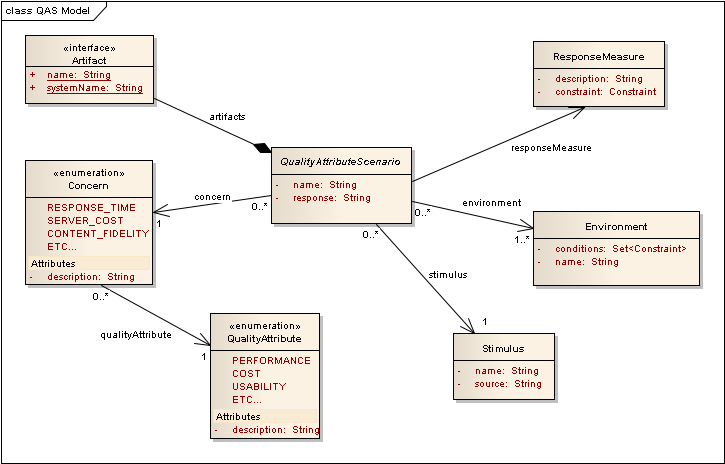
\includegraphics[width=1.00\textwidth]{images/QAS_Model.png}
			\caption{Modelo de QAS}
			\label{fig:QAS_Model}
		\end{figure}}		
		
		De todos los atributos que posee un QAS, el \textbf{Est�mulo}, el \textbf{Artefacto}, el \textbf{Entorno} y la
		\textbf{Cuantificaci�n de la Respuesta} son particularmente relevantes a los fines de establecer informaci�n �til para
		el mecanismo de auto reparaci�n. A lo largo de las pr�ximas secciones se detalla el uso que hace Arco Iris de esta
		informaci�n para modificar, optimizar y flexibilizar la auto reparaci�n llevada a cabo por Rainbow.

		\subsubsection{El Est�mulo en la Auto Reparaci�n}

			El \textbf{est�mulo} de un escenario normalmente se asocia a un evento desencadenado en el sistema por la acci�n del
			alguno de sus usuarios. Dicho evento es el punto de entrada del escenario, el disparador (interno o externo) que
			inicia la interacci�n con el sistema, y m�s particularmente, con el artefacto del escenario en cuesti�n. Por ejemplo,
			supongamos que en un sistema de administraci�n de cuentas bancarias un cliente intenta hacer una transferencia, en
			este caso la fuente del est�mulo ser�a el cliente y el est�mulo en s� mismo ser�a \emph{realizar transferencia}.
			En t�rminos de auto reparaci�n, generalmente el est�mulo se encuentra asociado a una operaci�n provista por el
			artefacto del sistema, el cual puede ser un componente, un conector o un sub sistema.

			Saber cu�l es el est�mulo de cada escenario permite optimizar la auto reparaci�n, ya que habiendo ocurrido
			determinado est�mulo, Arco Iris podr� detectar cu�les son los potenciales escenarios que pueden verse afectados y
			trabajar� verificando dicho subconjunto, acotando as� la cantidad de restricciones a verificar y, consecuentemente,
			optimizando el tiempo de la auto reparaci�n.

			Cabe destacar que tambi�n se ofrece la posibilidad de no especificar el est�mulo al configurar un escenario, es decir,
			se permite la opci�n de que el escenario aplique siempre, independientemente del est�mulo que haya impactado al sistema.
			Esto puede ser �til para casos gen�ricos, por ejemplo, si se requiere que el tiempo de respuesta experimentado por el
			usuario nunca sobrepase determinado umbral sin importar la funcionalidad del sistema que el usuario est� utilizando.
			En particular, se podr�a no configurar ning�n est�mulo en ning�n escenario, y en ese caso, Arco Iris verificar� que
			se satisfagan todos los escenarios en cada iteraci�n de la auto reparaci�n cada vez que un est�mulo perteneciente a
			cualquier escenario impacte sobre el sistema. Como puede se observar, es recomendable configurar el est�mulo
			espec�fico para cada escenario a fin de conseguir un funcionamiento m�s preciso del \emph{framework}.
			Entonces, a diferencia de Rainbow, quien debe verificar todas las restricciones en todo momento, Arco Iris permite
			refinar el conjunto de escenarios que pueden verse afectados por efecto del est�mulo que ocasiona el problema,
			reduciendo as� la cantidad de restricciones e invariantes a verificar.

			Para notificar sobre el est�mulo desencadente fue necesario extender los \emph{probes}, que, como ya mencionamos
			anteriormente, son los componentes encargados de extraer del sistema informaci�n referente a un
			determinado \emph{concern}, siendo los responsables tambi�n de volcar dicha informaci�n en un \emph{bus} compartido
			con otros \emph{probes}. De este bus, los \emph{gauges} consumir�n la informaci�n para luego interpretarla y
			transformarla en cambios en los valores de propiedades del modelo de la arquitectura.
			
			La extensi�n de los \emph{probes} implic� la necesidad de extender los \emph{gauges} de manera tal que puedan
			interpretar la nueva informaci�n sobre est�mulos agregada en cada uno de los mensajes creados por los \emph{probes}.
			
			Debido a que en el dise�o original de Rainbow, los mensajes que los \emph{probes} env�an a los \emph{gauges} son
			meras cadenas de texto, las extensiones realizadas a ambos componentes no presentaron mayores inconvenientes.
			
			Para graficar la diferencia en la implementaci�n que genera el agregar el est�mulo en la auto reparaci�n, se
			ejemplificar� una extensi�n a un \emph{probe} utilizado por Znn. El \emph{probe} escogido para extender y as� poder
			ser utilizado en Arco Iris consiste simplemente en invocar un servicio, esperar su respuesta y medir el tiempo
			transcurrido entre la invocaci�n y la respuesta; �sta ser� la informaci�n que el \emph{probe} reportar� en el
			\emph{bus} que luego consultar� e interpretar� el \emph{gauge} correspondiente.
			
			A continuaci�n se puede observar la configuraci�n original utilizada en Znn para instanciar un \emph{probe} del tipo
			ClientProxyProbe, esta configuraci�n se puede encontrar en el archivo \verb@probes.yml@, donde se declaran todos los
			\emph{probes} que ser�n instanciados al iniciar Rainbow:

			\begin{Verbatim}[gobble=4]
				probes: 
				ClientProxyProbe0: 
					alias: clientproxy 
					location: "localhost"
					type: java 
					javaInfo:
						class: org.sa.rainbow.translator.znews.probes.ClientProxyProbe
						period: 2000
						args.length: 1
						args.0: "http://delegate.oracle/"
			\end{Verbatim}

			Un ejemplo de la informaci�n que reporta un \verb@ClientProxyProbe@ con la configuraci�n presentada
			anteriormente podr�a ser:
			
			\begin{Verbatim}[gobble=4]
				[fri may 13 22:15:04 2011]<clientproxy> localhost: 1532 ms
			\end{Verbatim}
			
			Tanto la configuraci�n como la implementaci�n de \verb@ClientProxy@ son muy similares a las de su contraparte de Arco
			Iris, \verb@ClientProxyWithStimulus@. En el ap�ndice \ref{sec:probesCode} se pueden observar ambas implementaciones,
			mientras que la configuraci�n de una instancia de \verb@ClientProxyWithStimulus@ se puede observar a continuaci�n:

			\begin{Verbatim}[gobble=4]
				ClientProxyProbeWithStimulus0:
					alias: clientproxyWithStimulus
					location: "localhost" 
					type: java 
					javaInfo:
						class: ar.uba.dc.arcoiris.znn.probes.ClientProxyProbeWithStimulus
						period: 2000
						args.length: 2
						args.0: "http://delegate.oracle/"
						args.1: "delegateStimulus"
			\end{Verbatim}

			Por �ltimo, se muestra la informaci�n reportada por una instancia de\\
			\verb@ClientProxyWithStimulus@ con la configuraci�n que se acaba de presentar:
			
			\begin{Verbatim}[gobble=3]
			[fri may 13 22:15:04 2011]<clientproxyWithStimulus> localhost<stimulus:delegateStimulus>: 1532 ms
			\end{Verbatim}

			Algunas formas posibles de implementar \emph{probes} son:
			\begin{itemize}
			  \item Parseo e interpretaci�n de informaci�n existente en archivos de logs del sistema o en el servidor en el cual
			  se ejecuta.
			  \item Invocaciones idempotentes a servicios provistos por el sistema, con el fin de obtener m�tricas sobre las
			  respuestas.

			  \item El sistema a adaptar puede ofrecer servicios espec�ficos que provean informaci�n relevante para su auto
			  reparaci�n.
			\end{itemize}

		\subsubsection{El Artefacto en la Auto Reparaci�n}

			El \textbf{artefacto} se refiere al componente, conector o sub sistema afectado por el escenario, cualesquiera de
			ellos se encuentran descritos en el modelo de la arquitectura.

			La asociaci�n de un artefacto particular a un escenario permite acotar las propiedades sobre las cuales podr�
			predicar la \textbf{cuantificaci�n de la respuesta} (ver secci�n \ref{sec:responseMeasure}).

			La arquitectura presentada en Znn servir� para ejemplificar el concepto de artefacto. Cabe recordar que se trata
			de una arquitectura de estilo cliente-servidor, donde el componente de tipo \emph{ClientT} se define de la siguiente
			manera:

			\begin{Verbatim}[gobble=4]
				Component Type ClientT extends ArchElementT with {

				  Property deploymentLocation : string <<  default : string = "localhost"; >> ;

				  Property experRespTime : float <<  default : float = 100.0; >> ;

				  Property requestRate : float <<  default : float = 0.0; >> ;
				}
			\end{Verbatim}

			Suponiendo que se define el siguiente escenario:

			\begin{Quote}
				``Znn news debe servir el contenido de las noticias a los clientes en un tiempo de respuesta menor a 3 segundos en un
				entorno de operaci�n normal.''
			\end{Quote}

			Dado que en la arquitectura de Znn se modela a los clientes como componentes de la arquitectura, con una
			propiedad espec�fica \verb@experRespTime@ que representa el tiempo de respuesta experimentado por el usuario,
			claramente se observa que en este ejemplo \emph{ClientT} es el artefacto sobre el cual ha de predicar la verificaci�n
			de validez del escenario anteriormente detallado. M�s adelante, en la secci�n \ref{sec:responseMeasure}, se podr�
			observar c�mo se configura dicha restricci�n en un escenario de atributos de calidad.

		\subsubsection{El Entorno en la Auto Reparaci�n}
		\label{sec:environment}
		
			\subsubsubsection{El Concepto de Entorno en Rainbow}
			
				Si bien Rainbow utiliza el concepto de entorno y, para contribuir a la confusi�n del lector, lo llama
				\emph{scenario}, el mismo es configurable aunque est�tico, es decir, no se adapta din�micamente a los cambios
				que experimenta el sistema en tiempo de ejecuci�n.

				Rainbow implementa el entorno como una distribuci�n espec�fica de pesos relativos entre los distintos
				\emph{concerns} del sistema. A continuaci�n se muestra un ejemplo de un entorno (\emph{scenario}) de Rainbow
				utilizado por Znn:
		
				\begin{Verbatim}[gobble=3]
					weights:
						scenario 1:
							uR: 0.35
							uF: 0.4
							uC: 0.25
						scenario 2:
							uR: 0.5
							uF: 0.3
							uC: 0.2
						scenario 2b:
							uR: 0.5
							uF: 0.2
							uC: 0.3
				\end{Verbatim}
				
				Observar que cada entorno asigna un valor a cada \emph{concern} del sistema, en donde, en este caso, \verb@uR@
				representa al Tiempo de Respuesta, \verb@uF@ a la Fidelidad de la informaci�n y \verb@uC@ al Costo. Notar que la
				sumatoria de los pesos de los distintos \emph{concerns} para cada entorno debe ser igual a 1.

				Esta informaci�n debe ser configurada en el archivo de configuraci�n \emph{utilities.yml} utilizado por Rainbow. Aqu�,
				como se puede observar, se definen m�s de un entorno, uno de los cuales luego deber� ser seleccionado por el
				arquitecto en el archivo de configuraci�n \verb@rainbow.properties@ previo a la inicializaci�n, intentando
				predecir cu�les ser�n las condiciones en las que el sistema deber� responder. Este entorno es utilizado por
				Rainbow al momento de seleccionar una estrategia para reparar el sistema. En la secci�n \ref{sec:strategySelection}
				se explica en detalle su utilizaci�n.

			\subsubsubsection{El Entorno en Arco Iris y su Importancia para la Auto Reparaci�n}

				El concepto de \emph{scenario} de Rainbow es similar al concepto de Entorno planteada por QAS, el cual, a su vez
				ha sido extendido por Arco Iris. La diferencia fundamental radica en que, mientras en Rainbow el usuario debe
				predecir en qu� entorno operar� el sistema, Arco Iris lo detectar� autom�ticamente. M�s adelante en esta secci�n, se
				explicar� en detalle c�mo se lleva a cabo esta tarea.

				Concentr�ndonos ahora �nicamente en Arco Iris, y de acuerdo a la definici�n de QAS, se define al \textbf{Entorno de
				Ejecuci�n}, o simplemente, \textbf{Entorno} como el estado en el que el sistema se encuentra cuando recibe el
				est�mulo que desencadena el escenario. A modo de ejemplo: al recibir una solicitud de creaci�n de una cuenta
				bancaria el sistema puede encontrarse en ``operatoria normal'', en ``alta carga'' o quiz�s tal vez se encuentre
				``fuera de operaci�n''.
				
				El entorno condiciona la validez del escenario en cuesti�n a que el sistema se encuentre en un determinado estado,
				ya que, por ejemplo, una respuesta esperada aceptable o f�cil de cumplir bajo un entorno puede ser inaceptable o muy
				costosa en otro.
	
				En el escenario planteado en la secci�n anterior, si el sistema se encontrase en un entorno de ``alta carga'' el
				escenario se satisfar�a trivialmente, ya que para considerar dicho escenario el sistema deber�a encontrarse en un
				entorno de ``operaci�n normal''.
				
				De esta manera, el entorno del escenario es un elemento que permite a Arco Iris optimizar la b�squeda de escenarios
				que no se satisfacen en un determinado instante ante la recepci�n de un est�mulo, ya que se ignorar�n aquellos
				escenarios cuyo entorno posea condiciones que no se cumplen en dicho instante. M�s adelante se profundizar� sobre
				dichas condiciones.

			\subsubsubsection{Escenarios modelados con varios entornos}

				Si bien el concepto de escenario de atributo calidad, tal cual fue definido en la secci�n \ref{sec:QAS}, incluye
				�nicamente un s�lo entorno, en Arco Iris se ha decidido modelar al escenario con una \textbf{colecci�n de
				entornos}. A fin de justificar esta decisi�n de dise�o, supongamos que un \emph{stakeholder} desea que un
				determinado escenario sea v�lido en varios entornos. En ese caso, siguiendo la definici�n estricta de QAS d�nde un
				escenario s�lo posee un entorno, el \emph{stakeholder} deber�a crear varios escenarios id�nticos, todos ellos
				difiriendo �nicamente en su entorno. Esto es claramente inconveniente, m�s a�n considerando que la cantidad de
				entornos configurables por el usuario no est� acotada, lo cual podr�a llevar a una explosi�n innecesaria de
				escenarios cuasi id�nticos.
				
				Ahora bien, habiendo dicho lo anterior, tambi�n puede ocurrir la situaci�n d�nde, de acuerdo al entorno de
				ejecuci�n, se desea tener en cuenta subconjuntos distintos de estrategias de reparaci�n. En este caso, no existe
				otra opci�n m�s que configurar distintos escenarios.
				
				Cabe destacar que, a fines de simplificar el problema y acotar as� el alcance de este trabajo, en el modelo de
				Arco Iris se establece una restricci�n no poco importante: se presupone que el usuario de Arco Iris no cargar� en el
				sistema entornos cuyas condiciones de aplicabilidad tengan intersecci�n no nula. Esta simplificaci�n, si bien no
				representa mayor problema a los fines de este trabajo, s� restringe futuras extensiones del mismo. La naturaleza de
				tal restricci�n y una posible soluci�n son abordadas en detalle en la secci�n \ref{sec:flexibilizacionEntorno}.

			\subsubsubsection{Estructura y Caracter�sticas del Entorno}

				La estructura del entorno consiste en:
	
				\begin{itemize}
					\item Un nombre,
					\item Un conjunto de condiciones, y
					\item Un mapa \verb@<Concern, Peso>@
				\end{itemize}
	
				El \textbf{nombre} es simplemente una cadena de texto que sirve para r�pidamente identificarlo.
	
				Las \textbf{condiciones} son predicados que predican sobre los valores de las propiedades del modelo de la
				arquitectura del sistema en tiempo de ejecuci�n. Para que un sistema en ejecuci�n se encuentre en un determinado
				entorno, deben satisfacerse \textbf{todas} sus condiciones. Para m�s informaci�n sobre la implementaci�n en Arco
				Iris de las condiciones del entorno, ver la secci�n \ref{sec:modeloRestriccionesArcoIris}.
								
				El objetivo del \textbf{mapa de pesos} presente en la estructura del entorno es el de definir la importancia
				relativa de cada \emph{concern} cuando el sistema se encuentra en el entorno en cuesti�n. Dicho mapa debe contener
				todos los \emph{concerns} definidos para el sistema y la suma de sus pesos debe ser igual a uno. En la secci�n
				\ref{sec:arcoIrisStrategyScoring} se detalla de qu� manera Arco Iris hace uso de estos pesos para escoger la mejor
				estrategia de reparaci�n.
							
			\subsubsubsection{El Entorno ``ANY''}

				Una caracter�stica particular de Arco Iris es la de permitir expresar, mediante la selecci�n de un pseudo-entorno
				preexistente denominado ``ANY'', que un determinado escenario aplica bajo cualquier entorno. Esto es equivalente a que
				el entorno del escenario no posea condici�n alguna, es decir, que el escenario aplica siempre, trivialmente, sin
				importar las condiciones actuales del sistema en ejecuci�n. Esto puede resultar �til en algunos casos ya que simplifica
				la configuraci�n del escenario, pero es importante tener en cuenta que, por otro lado, el rendimiento de la auto
				reparaci�n se ver� reducido puesto que el configurar uno o m�s entornos espec�ficos por escenario otorga mayor precisi�n
				al permitir establecer la importancia (peso relativo) de cada \emph{concern} seg�n el estado en el que el sistema se
				encuentre.
	
				El entorno ``ANY'' ser� asignado autom�ticamente al escenario si el usuario no especifica ning�n entorno o, si por
				el contrario, decide expl�citamente que el escenario aplique \textbf{en cualquier entorno de ejecuci�n}. En
				cualquiera de los dos casos, Arco Iris asignar� a todos los \emph{concerns} el mismo peso, con la intenci�n de
				evitar otorgarle m�s importancia a alg�n \emph{concern} en particular. Esta decisi�n de equidistribu�r los pesos
				relativos por \emph{concern} es, desde ya, arbitraria y se reconoce una posibilidad de mejora en vistas de un
				trabajo futuro. Para m�s informaci�n, ver \ref{asignacionEquidistribuidaPesos}.
	
				Para ejemplificar la importancia de configurar un entorno correctamente y no hacer abuso del pseudo-entorno ``ANY'',
				considerar, por ejemplo, un sistema el cual se encuentra bajo excesiva carga, y los \emph{stakeholders} consideran
				que bajo tales circunstancias lo m�s prioritario es optimizar la \emph{performance} del sistema. En ese caso, de no
				especificar el entorno no ser� posible otorgarle mayor peso a la \emph{performance} por sobre otros \emph{concerns},
				quedando �nicamente la opci�n de aumentar la prioridad\footnote{se profundizar� sobre este tema en la secci�n
				\ref{sec:priority}} de todos los escenarios relacionados con dicho \emph{concern}, tergiversando as� dicha
				informaci�n, ya que en realidad lo �ptimo ser�a asignarle m�s peso al \emph{concern performance} en el entorno de
				``Alta Carga''. Puesto de otra manera, el establecer que un escenario aplica en cualquier entorno, tiene como
				consecuencia que Arco Iris interprete que el entorno carece de importancia, dejando de lado los pesos de los
				\emph{concerns} y distribuyendo equitativamente su importancia relativa, lo cual es equivalente a que el concepto de
				\emph{concern} no exista.

		\subsubsection{La Cuantificaci�n de la Respuesta en la Auto Reparaci�n}
			\label{sec:responseMeasure}

			La \textbf{cuantificaci�n de la respuesta} (o, en ingl�s, \emph{Response Measure}) es quiz�s la propiedad m�s
			importante de un escenario, de ella surgen las restricciones que deben ser evaluadas para que, en caso de no
			cumplirse, se lance la auto reparaci�n. En pocas palabras, la cuantificaci�n de la respuesta se define como la
			m�trica seg�n la cual se decide si la respuesta del sistema ante un determinado est�mulo es aceptable o no.
			
			Para que un escenario se considere bien formado debe quedar claro cu�l es la m�trica o manifestaci�n observable de su
			respuesta que se debe satisfacer. Latencia y \emph{throughput} son ejemplos de manifestaciones sobre las cuales puede
			predicar la cuantificaci�n de la respuesta.

			Para graficar la importancia de contar con una cuantificaci�n de la respuesta precisa, supongamos que contamos con la
			siguiente definici�n:

			\begin{Quote}
				``El sistema debe ser modificable para poder incorporar un nuevo generador de eventos discretos''
			\end{Quote}

			Esta premisa no es suficiente para medir el �xito de la incorporaci�n de la nueva funcionalidad solicitada, ya que
			con suficiente tiempo y recursos, casi cualquier modificaci�n es posible. Este escenario requiere una m�trica, como
			por ejemplo: \emph{``Utilizando 160 horas/hombre''}. Esto fuerza al arquitecto a asegurar que el sistema sea
			modificable bas�ndose en un criterio bien definido y con una m�trica aplicable.

			Con respecto a la implementaci�n, el componente m�s importante de la cuantificaci�n de la respuesta es la
			restricci�n, cuyo modelo en Arco Iris fue anteriormente explicado en la secci�n
			\ref{sec:modeloRestriccionesArcoIris}.
			
			En Arco Iris las restricciones se sit�an en el contexto de un escenario de atributo de calidad, proveyendo as� mayor
			visibilidad a los \emph{stakeholders}, las cuales antes se encontraban implementadas en el modelo de la arquitectura
			utilizando el lenguaje Acme, y consecuentemente, eran s�lo conocidas y modificadas por los arquitectos y/o t�cnicos
			responsables de configurar el \emph{framework}.

			El siguiente ejemplo ha sido extra�do de la arquitectura de Znn. Aqu� se puede observar de qu� manera se implementan
			las restricciones al utilizar Rainbow:
			
			\begin{Verbatim}[gobble=4] 
				Component Type ClientT {
					Property experRespTime : float <<  default : float = 100.0; >> ;
					rule primaryConstraint = invariant self.experRespTime <= 1000;
				}
			\end{Verbatim}

			Es importante recordar que en Rainbow, una vez que se detect� que la auto reparaci�n debe ser lanzada debido a una
			restricci�n que dej� de cumplirse, se volver�n a evaluar todas las restricciones definidas en las precondiciones de
			\textbf{todas las estrategias} para verificar si aplican o no dependiendo del estado actual del sistema. A
			continuaci�n se muestra un ejemplo extra�do de Znn de una estrategia y su precondici�n:

			\begin{Verbatim}[gobble=4]
				import model "ZNewsSys.acme" { ZNewsSys as M};
				...
				define boolean cViolation =
				    exists c : ClientT in M.components | c.experRespTime > 1000;
				...
				strategy BruteReduceResponseTime
				[ cViolation ] {
					...
					execute some tactic...
					...
				}
			\end{Verbatim}

			Como se puede observar, tanto la restricci�n en el modelo que desencaden� la auto reparaci�n como la precondici�n de
			la estrategia son equivalentes, por lo que se duplica la l�gica aumentando el costo de procesamiento, haciendo que la
			reparaci�n sea m�s costosa y menos escalable. Adem�s al duplicar la configuraci�n, el costo de mantener el
			\emph{framework} es mayor.

			En Arco Iris no ser� necesario contar con las precondiciones de las estrategias, ya que el conocimiento de cu�les
			estrategias son capaces de reparar una determinada condici�n se encuentra plasmado en cada escenario. En definitiva, al
			utilizar Arco Iris el usuario accede a la posibilidad de configurar el comportamiento esperado del sistema mediante
			la cuantificaci�n de la respuesta de cada escenario, tarea que se ve sumamente facilitada al utilizar Arco Iris UI
			(ver secci�n \ref{sec:arcoIrisUI}).

			Otra diferencia esencial con respecto al uso que Rainbow y Arco Iris hacen de las restricciones, es el momento en
			el que se aplican. Hemos visto anteriormente que Rainbow posee un componente llamado \emph{``Architecture
			Evaluator''}, cuya responsabilidad consiste en verificar de a intervalos la arquitectura del modelo, siempre y
			cuando �ste haya sufrido algunas modificaci�n y no se est� ya ejecutando un proceso de auto reparaci�n, esto implica
			verificar absolutamente todas las restricciones del modelo. Arco Iris, en cambio, al descubrir un cambio en el
			modelo, verifica que los escenarios se satisfagan, pero no todos los escenarios, sino solamente aquellos cuyo
			est�mulo coincida con el que desencaden� la actualizaci�n del modelo, optimizando as� de manera dr�stica la cantidad
			de restricciones a verificar, lo que hace m�s escalable la auto reparaci�n.

	\subsection{Modelo Extendido de QAS}
	\label{sec:modeloExtensionQAS}
	
		Hasta aqu� se ha detallado el uso que Arco Iris hace del modelo b�sico de QAS, pero como se mencion� anteriormente,
		es necesario extender este modelo para agregar informaci�n de auto reparaci�n propiamente dicha.
		
		En la figura \ref{fig:Arco_Iris_QAS_Model} se puede observar el modelo del \textbf{escenario de auto reparaci�n}\\
		(\verb@SelfHealingScenario@), el cual, adem�s de ser un QAS tiene toda la informaci�n y la l�gica necesaria para que
		Arco Iris pueda llevar a cabo su objetivo de flexibilizar la auto reparaci�n.

		\afterpage{\clearpage
		\begin{figure}[H]
			\centering
				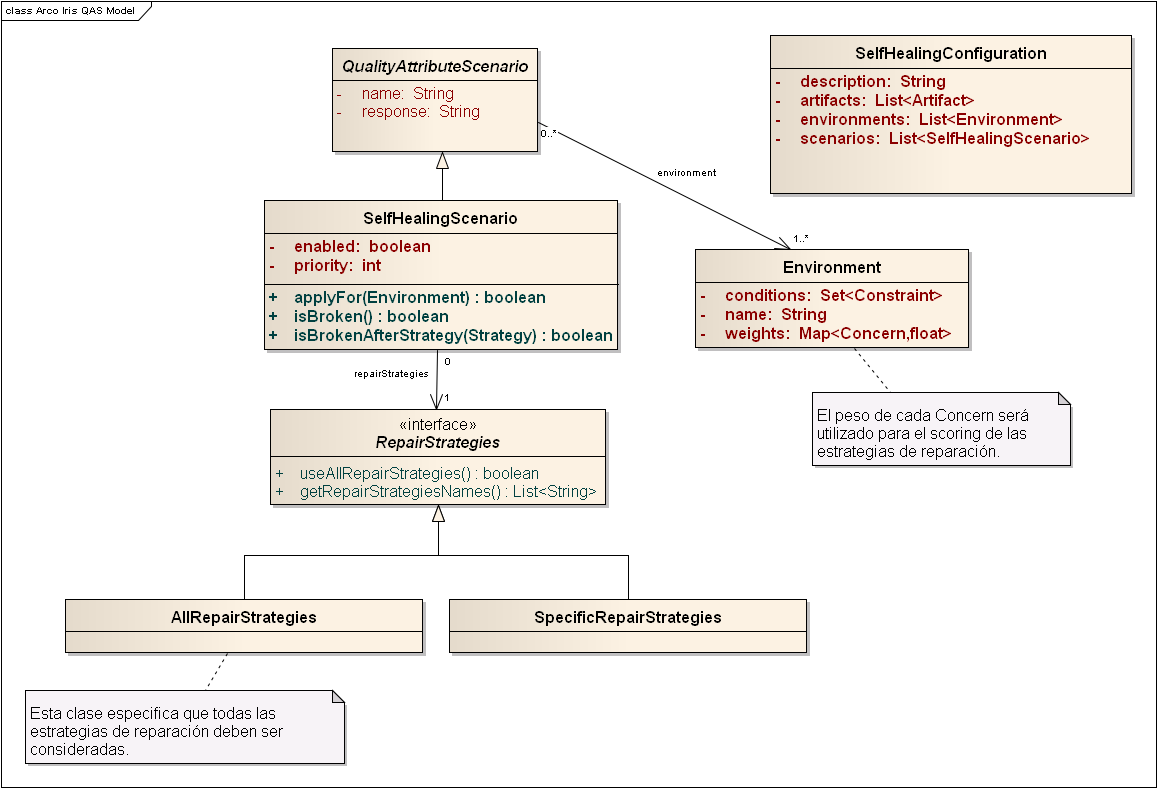
\includegraphics[width=1.00\textwidth]{images/Arco_Iris_QAS_Model.png}
			\caption{Modelo de Arco Iris}
			\label{fig:Arco_Iris_QAS_Model}
		\end{figure}}

		Los escenarios de auto reparaci�n pueden ser deshabilitados, considerando Arco Iris solamente aquellos escenarios
		habilitados al momento de reparar el sistema.

		Otra propiedad utilizada por Arco Iris y que no forma parte de la definici�n original de un QAS, es la prioridad. Cada
		\verb@SelfHealingScenario@ tiene preestablecida su prioridad (ver secci�n \ref{sec:priority} para m�s detalle). Un
		escenario de Arco Iris tambi�n tiene el conocimiento necesario para determinar si se satisface seg�n las condiciones
		actuales del sistema, y tambi�n para predecir si seguir� satisfaciendose luego de una potencial aplicaci�n de una
		estrategia en particular.

		Otra extensi�n a QAS implementada por Arco Iris para optimizar la auto reparaci�n consiste en que cada escenario
		conozca las estrategias que el arquitecto del sistema y los \emph{stakeholders} consideran son capaces de reparar el
		escenario en caso de que este haya dejado de satisfacerse. En la secci�n \ref{sec:strategies} puede verse en detalle
		c�mo Arco Iris explota esta informaci�n.

		Por �ltimo, es importante recordar que se ha extendido el concepto de \textbf{entorno} utilizado por QAS, el cual
		pasa a contar, adem�s de con su nombre, con un conjunto de condiciones que ser�n utilizadas para saber si un determinado
		escenario aplica, dado su entorno, para las condiciones actuales del sistema, y adem�s ser� capaz de determinar la
		importancia de cada \emph{concern} para el caso en el que el sistema en ejecuci�n se encuentre en este entorno. Esta
		extensi�n ya fue explicada en detalle en la secci�n \ref{sec:environment}.	


	\subsection{Prioridades entre Escenarios}
	\label{sec:priority}
	
		\todo{TURCO Y JONY: continuar revisando desde aca}

		Una caracter�stica distintiva de Arco Iris, la cual no posee contraparte alguna en Rainbow, es la de ofrecer la
		posibilidad de \textbf{priorizar escenarios} asign�ndoles prioridades relativas, de modo tal que al momento de escoger
		una estrategia de auto reparaci�n la estrategia seleccionada no comprometa a alguna otra funcionalidad de la aplicaci�n
		considerada m�s importante seg�n la visi�n de los \emph{stakeholders}.

		Para lograr lo antedicho, a cada escenario se le asigna una prioridad, representada por un valor num�rico entero
		positivo que es inversamente proporcional a la importancia que se desea asignarle al escenario. Por ejemplo, un
		escenario con prioridad 2 es considerado m�s prioritario que otro con prioridad 6.
		
		Si bien esta nueva funcionalidad abre nuevas posibilidades al usuario, por otro lado, la misma debe manejarse con sumo
		cuidado ya que es probable que, al configurar escenarios con prioridades \emph{muy grandes}, �stos no tengan
		pr�cticamente ning�n peso al momento de seleccionar la estrategia de auto reparaci�n a aplicar, con lo cual dichos
		escenarios nunca ser�n reparados, careciendo de sentido as� su existencia.

		La prioridad del escenario es una propiedad fundamental para el correcto funcionamiento de Arco Iris, veremos su
		importancia al detallar de qu� manera Arco Iris selecciona la estrategia que aplicar� para reparar el sistema en la
		secci�n \ref{sec:strategySelection}. Por esta raz�n ser� de extrema importancia la correcta configuraci�n de cu�les
		ser�n los escenarios prioritarios: �stos deber�n reflejar la importancia fundamental de los servicios ofrecidos por el
		sistema seg�n las expectativas de los usuarios finales. Se recomienda realizar la asignaci�n de la prioridad de cada
		escenario como un paso m�s del Quality Attribute Workshop (QAW), para m�s detalle ver la secci�n \ref{sec:QAW}.

	\subsection{Estrategias y su Relaci�n con los Escenarios}
	\label{sec:strategies}

		Antes de profundizar en c�mo Arco iris utiliza las estrategias implementadas para reparar escenarios, recordemos
		brevemente c�mo se utilizan las mismas en Rainbow.

		Las estrategias en Rainbow tienen un conjunto de precondiciones que nos indican si dicha estrategia puede ser
		utilizada para reparar el sistema en un determinado momento. Esto implica que, en cuanto Rainbow detecta un problema
		en el sistema, deba recorrer todas las estrategias existentes para ver si son aplicables para las condiciones
		actuales. En otras palabras, Rainbow no tiene forma de determinar \textbf{a priori} la utilidad de una estrategia en
		el preciso momento en que una o m�s restricciones sobre el modelo de la arquitectura del sistema se dejan de cumplir.
		
		Por ejemplo, para que una estrategia que soluciona problemas de \emph{performance} no sea tenida en cuenta al reparar un
		escenario relacionado a un atributo de calidad distinto, como por ejemplo el costo, debe agregarse una precondici�n como
		la siguiente en la estrategia:

		\begin{Verbatim}[gobble=4]
			strategy SimpleReduceResponseTime
			  [ responseTimeConstraintViolation ] {
			  ...
			}
		\end{Verbatim}

		Donde \emph{responseTimeConstraintViolation} es un predicado que permite determinar si existe alg�n cliente cuyo tiempo
		de respuesta haya sobrepasado el tiempo de respuesta m�ximo permitido:

		\begin{Verbatim}[gobble=4]
			define boolean responseTimeConstraintViolation =
				exists c : T.ClientT in M.components | c.experRespTime > M.MAX_RESPTIME;
		\end{Verbatim}

		Con respecto al anterior ejemplo, es importante remarcar que, en caso de que el problema que se est� intentando reparar
		no tenga relaci�n con la \emph{performance}, Rainbow deber� de todos modos chequear el tiempo de respuesta de todos los
		clientes, mientras que en Arco Iris existe la posibilidad de evitarlo al configurar correctamente las estrategias
		asociadas a cada escenario.
			
		Como ya se ha mencionado, en Arco Iris si bien se utilizan el mismo tipo de t�cticas y estrategias que en Rainbow (i.e.
		modeladas con Stitch), se propone desacoplar la detecci�n del problema de su soluci�n utilizando como medio para ello
		los escenarios de atributos de calidad. All� se definen las condiciones para la detecci�n del problema (restricciones
		dentro de la cuantificaci�n de la respuesta) y se referenciar�n las posibles estrategias de reparaci�n a ser
		consideradas para su ejecuci�n, en el caso de que el escenario en cuesti�n se vea comprometido. De esta forma, las
		estrategias quedan exentas de conocer cu�les son las circunstancias en las que su ejecuci�n tiene sentido. Esto permite
		al arquitecto tener un mayor control sobre las estrategias a ejecutar en determinadas condiciones, ya que al situarse en
		un escenario concreto, �l sabr� cuales ser�n las soluciones m�s adecuadas bas�ndose en el entorno del sistema y en la
		prioridad del escenario en cuesti�n.
				
		Cabe acotar que Arco Iris tambi�n ofrece la posibilidad de configurar el mismo comportamiento brindado por Rainbow: esto
		se logra simplemente indicando la opci�n que representa a ``todas las estrategias existentes'' cuando se configura el
		escenario (una forma sencilla de especificar �sto, utilizando Arco Iris UI, se explica en la secci�n
		\ref{sec:strategySelectionUI}).
				
		Al igual que en Rainbow, las estrategias poseen la informaci�n necesaria para permitir \textbf{simular su aplicaci�n} y
		estimar en que condiciones quedar�a el sistema luego de haber sido aplicadas. Esta informaci�n ser� utilizada para la
		estimaci�n de la nueva ``utilidad del sistema'', concepto sobre el cual, se profundizar� en la secci�n
		\ref{sec:systemUtility}.

		En Arco Iris, para poder escribir estrategias que involucren varias t�cticas, el usuario contar� con un mecanismo que
		le permitir� verificar si los escenarios de un determinado \emph{concern}, y que han sido marcados para reparar,
		siguen a�n sin cumplirse. En base a esta informaci�n la estrategia podr� decidir c�mo continuar su ejecuci�n. A
		continuaci�n se muestra un ejemplo de su utilizaci�n:

		\begin{Verbatim}[gobble=4]
				import op "org.sa.rainbow.adaptation.ArcoIrisAdaptationManager";
				...
				define boolean RESP_TIME_STILL_BROKEN =
						ArcoIrisAdaptationManager.isConcernStillBroken("RESPONSE_TIME");
				...
				/*
				 * This Strategy will drop fidelity once, observe, then drop again if necessary.
				 */
				strategy BruteReduceResponseTime
				[ styleApplies ] {
				  t0: (true) -> lowerFidelity(2, 100) @[5000 /*ms*/] {
				    t1: (!RESP_TIME_STILL_BROKEN) -> done;
				    t2: (RESP_TIME_STILL_BROKEN) -> lowerFidelity(2, 100) @[8000 /*ms*/] {
				      t2a: (!RESP_TIME_STILL_BROKEN) -> done;
				      t2b: (default) -> TNULL;  // in this case, we have no more steps to take
				    }
				  }
				}
				...
			\end{Verbatim}

		C�mo se puede observar en el c�digo, para que este mecanismo funcione, es necesario importar la funci�n
		\verb@isConcernStillBroken@ de la clase \verb@ArcoIrisAdaptationManager@, cuya implementaci�n se ver� a continuaci�n.
		Notar que el usuario solamente deber� indicar cual es el \emph{concern} de su inter�s:

		\begin{Verbatim}[gobble=4]
				public static boolean isConcernStillBroken(String concernString) {
					Concern concern = Concern.valueOf(concernString);
					doLog(Level.INFO, "Is Concern " + concern + " Still Broken?");

					boolean result = false;
					for (SelfHealingScenario scenario : currentBrokenScenarios) {
						if (scenario.getConcern().equals(concern) &&
								scenarioBrokenDetector4CurrentSystemState.isBroken(scenario)) {
							result = true;
							break;
						}
					}
					doLog(Level.INFO, "Concern " + concern + (result == true ?
							" Still Broken!" : " Not Broken Anymore!!!"));
					return result;
				}
		\end{Verbatim}

	\subsection{Activaci�n del Mecanismo de Auto Reparaci�n}

		\todo{Explicar que cuando se lanza la adaptacion no se reciben mas actualizaciones al modelo hasta una vez finalizada
		la adaptacion comenzada}

		Con el nuevo enfoque presentado en este trabajo, d�nde el \emph{Escenario} es el concepto central, es necesario
		establecer cambios en la l�gica aplicada por el \emph{framework} a la hora de decidir en qu� momento es necesario
		intentar auto reparar el sistema (i.e. evaluar sus restricciones o invariantes).

		En Rainbow, las restricciones del sistema se encuentran embebidas en la descripci�n arquitect�nica de sus componentes,
		m�s precisamente en el modelo de la arquitectura, el cual se describe utilizando el lenguaje de descripci�n de
		arquitectura ACME (\ref{sec:acme}). Por ejemplo, para determinar que el tiempo de respuesta no debe exceder un umbral
		determinado es necesario definir una restricci�n en el componente que posee dicha propiedad, como se puede observar en
		el siguiente ejemplo tomado de la arquitectura de Znn:

		\begin{Verbatim}[gobble=4]
				Component Type ClientT extends ArchElementT with {

					Property experRespTime : float <<  default : float = 100.0; >> ;

					rule primaryConstraint = invariant self.experRespTime <= 1000;
				}
		\end{Verbatim}

		En Arco Iris ya no ser� necesario definir estas \emph{constraints} en la arquitectura, desacoplando as� la arquitectura
		del sistema de la definici�n de condiciones a evaluar para lanzar la auto reparaci�n. Ahora las restricciones estar�n
		presentes en la \emph{Cuantificaci�n de la Respuesta}(\ref{sec:responseMeasure}) de cada escenario. Al cambiar el modo
		de definir las \emph{constraints} se intenta adem�s dar mayor visibilidad a los \emph{stakeholders} del sistema, para
		esto Arco Iris a�ade la posibilidad de definir las restricciones de manera visual utilizando Arco Iris UI
		(\ref{sec:arcoIrisUI}), para m�s detalle ver la secci�n \ref{sec:arcoIrisUI_constraints}. Todo esto hace que los
		\emph{stakeholders} puedan acceder de manera sencilla a las restricciones a las cuales debe acatarse el sistema,
		pudiendo editarlas sin la necesidad de poseer conocientos sobre las tecnolog�as utilizadas por el sistema o por el
		\emph{framework} de auto reparaci�n.
		Para determinar si el sistema necesita auto repararse, Rainbow utiliza una funcionalidad ofrecida por ACME, que
		permite evaluar las restricciones descritas en el modelado de la arquitectura, para esto ACME provee una herramienta
		llamada \emph{Type Checker}. A continuaci�n podemos observar c�mo Rainbow se sirve de esta utilidad para decidir si
		debe lanzar la auto reparaci�n o no:

		\begin{Verbatim}[gobble=4]
				public void evaluateConstraints () {
					IAcmeTypeChecker typechecker = m_acmeEnv.getTypeChecker();
					if (typechecker instanceof SynchronousTypeChecker) {
						SynchronousTypeChecker synchChecker = (SynchronousTypeChecker) typechecker;
						synchChecker.typecheckAllModelsNow();
						m_constraintViolated = !synchChecker.typechecks(m_acmeSys);
						if (m_constraintViolated) {
							Set<?> errors = m_acmeEnv.getAllRegisteredErrors();
							Oracle.instance().writeEvaluatorPanel(m_logger, errors.toString());
						}
					}
				}
		\end{Verbatim}

		Recordemos que en Arco Iris hemos desacoplado el modelado de la arquitectura de las restricciones que deben
		satisfacerse, por lo cual no podremos utilizar la funcionalidad provista por ACME. Para suplir esto, y tambi�n para
		poder permitir incluir toda la informaci�n necesaria en los escenarios y que la misma pueda ser visualizada y editada
		por todos los \emph{stakeholders} involucrados, hemos desarrollado nuestra propia implementaci�n de las restricciones,
		la cual permiten expresar las mismas \emph{constraints} definidas en ACME, y en caso de ser necesario agregar un nuevo
		tipo de restricci�n permite f�cilmente incorporar una nueva implementaci�n implementando una interfaz muy sencilla
		(ver el ap�ndice \ref{sec:numericBinaryRelationalConstraintCode}). Estas \emph{constraints} ser�n de vital importancia
		a la hora de activar el mecanismo de auto reparaci�n. Al iniciar, Arco Iris leer� todos los escenarios definidos, y
		armar� un mapa que le permitir� optimizar las verificaciones recurrentes de los escenarios ante la llegada de cada
		est�mulo. El mapa almacena todos los escenarios correspondientes a cada est�mulo, as�, ante la invocaci�n de un
		est�mulo en el sistema, Arco Iris s�lo deber� verificar que se cumplan los escenarios relacionados con dicho est�mulo,
		acotando as� de manera sustancial la cantidad de chequeos a realizar. Recordar que en Rainbow, ante cualquier
		modificaci�n en el estado de la arquitectura, es necesario verificar todas las restricciones definidas para la auto
		reparaci�n.

		Paso a paso el proceso de activaci�n de la auto reparaci�n en Arco Iris consiste en lo siguiente:
		\begin{enumerate}
			\item El sistema en ejecuci�n recibe la invocaci�n de un est�mulo.
			\item Se modifican las propiedades del Modelo de la Arquitectura del sistema como consecuencia del est�mulo.
			\item Se buscan los escenarios que pueden verse afectados ante dicho est�mulo.
			\item Una vez identificados los escenarios potencialmente afectados, se verifica que se cumplan sus restricciones,
			siempre y cuando el entorno del escenario coincida con el actual, de lo contrario el escenario se considera
			verificado autom�ticamente.
			\item En el caso de detectar que uno o m�s escenarios dejaron de cumplirse, se lanzar� la auto reparaci�n del
			sistema, para lo cual la primer tarea a realizar ser� decidir cual ser� la estrategia m�s conveniente a aplicar, o
			sea, cual estrategia maximiza la \emph{Utilidad del Sistema} en entorno de operaci�n actual.
		\end{enumerate}

	\subsection{Selecci�n de Estrategia}
	\label{sec:strategySelection}

		Arco Iris selecciona la estrategia a aplicar para reparar el sistema de un manera sustancialmente diferente con
		respecto a Rainbow. Para comenzar, Rainbow considerar� todas las estrategias existentes mientras que Arco Iris se
		limitar� a considerar las estrategias propuestas en el escenario que se ha dejado de satisfacer, esto obviamente
		reduce ampliamente el universo de posibilidades reduciendo as� el tiempo de la autoreparaci�n. Recordemos que la
		configuraci�n de Arco Iris tambi�n ofrece la posibilidad de considerar todas las estrategias existentes, simulando
		as� el comportamiento ofrecido por Rainbow evit�ndose el usuario de realizar una configuraci�n m�s rigurosa en
		desmedro de la \emph{performance} de la autoreparaci�n.

		Por su parte, Rainbow descartar� las estrategias cuyas condiciones no se satisfagan, est�s condiciones generalmente se
		corresponden con la restricci�n que ha dejado de cumplirse, por lo cual su l�gica se encuentra duplicada en el
		modelado de la arquitectura y en la condici�n de la estrategia, consideremos la siguiente estrategia tomada de Znn a
		modo de ejemplo:

		\begin{Verbatim}[gobble=3]
			define boolean cViolation = exists c : T.ClientT in M.components |
					c.experRespTime > M.MAX_RESPTIME;
	
			strategy QuickDirtyReduceResponseTime
			[ cViolation ] {
			  t0: (/*hiLoad*/ cViolation) -> lowerFidelity(2, 100) @[2000 /*ms*/] {
			    t1: (!cViolation) -> done;
			  }
			}
		\end{Verbatim}

		Donde \emph{cViolation} representa la misma l�gica dispuesta en el invariante determinado al modelar la arquitectura:
		\begin{Verbatim}[gobble=3]
			Component Type ClientT extends ArchElementT with {
	
		        Property experRespTime : float <<  default : float = 100.0; >> ;
				...
		        rule primaryConstraint = invariant self.experRespTime <= MAX_RESPTIME;
		    }
		    ...
		    Property MIN_RESPTIME : float = 100.0;
		\end{Verbatim}

		En Arco Iris, una vez que se ha detectado que un escenario ha dejado de satisfacerse, simplemente se toman como
		estrategias candidatas las definidas en �l, evitando as� el \emph{overhead} de volver a verificar las condiciones.

		Ahora bien, una vez determinado el subconjunto de estrategias a considerar, es necesario asignarle un valor a cada
		una para poder seleccionar la estrategia que luego de ser aplicada maximice el rendimiento del sistema, para esto
		definiremos el concepto de \emph{Utilidad del Sistema} y mostraremos la heur�stica propuesta para su c�lculo tanto en
		Rainbow como en Arco Iris.

		\subsubsection{Utilidad del Sistema}
		\label{sec:systemUtility}

			Rainbow utiliza la teor�a de la utilidad, concepto forjado en el estudio de la econom�a, que permite asignar una
			medida relativa de satisfacci�n sobre un sistema sobre el cual es necesario medir el impacto ante cambios
			determinados. Una vez definida esta medida, permite hablar con sentido sobre incrementar o decrementar la utilidad del
			sistema, y as� explicar el impacto de una determinada decisi�n sobre el comportamiento del sistema.

			La idea principal al utilizar la teor�a de la utilidad en Rainbow es enumerar expl�citamente los atributos de calidad
			para las cuales se est� evaluando la t�cnica de autoreparaci�n; luego, indicar el peso dado a cada dimensi�n (ver
			\ref{sec:priority}). Por otro lado, al valor de cada atributo de calidad en el sistema se le aplicar� la funci�n
			de utilidad correspondiente, la cual se encuentra definida para cada \emph{concern} en el archivo de configuraci�n de
			Rainbow llamado \emph{utilities.yml}. Ejemplo de funci�n de utilidad correspondiente al tiempo de respuesta tomada de
			Znn:

				\begin{Verbatim}[gobble=4]
				utilities:
				  uR:
				    label: Average Response Time
				    mapping: "[EAvg]ClientT.experRespTime"
				    description: "Client experienced response time in milliseconds, R, defined as
				    				a float property 'ClientT.experRespTime' in the architecture"
				    utility:
				      0: 1.00
				      100: 1.00
				      200: 0.99
				      500: 0.90
				      1000: 0.75
				      1500: 0.50
				      2000: 0.25
				      4000: 0.00
				\end{Verbatim}

			Por �ltimo, Rainbow realizar� la suma de estos valores ponderados por el peso de cada \emph{concern}, el resultado de
			esta suma recibir� el nombre de \emph{Utilidad del Sistema}. Pseudoc�digo del c�lculo de la utilidad del sistema en
			Rainbow:

			\begin{Verbatim}[gobble=4]
				puntaje = 0
				valoresPorConcern = valores actuales del sistema para cada concern
				Por cada concern
					uf = Funcion de Utilidad para el concern actual
					valorConcern = valoresPorConcern.get(concern)
					valorUtilidad = uf(valorConcern)
					valorPonderado = valorUtilidad * peso asignado al concern en la configuraci�n est�tica de Rainbow
					puntaje = puntaje + valorPonderado
			\end{Verbatim}

			En el caso de Rainbow esta medida permitir� tener una noci�n de como impactar� una determinada estrategia sobre el
			sistema, para lo cual cada t�ctica deber� explicitar los \emph{concerns} sobre los cuales impacta y en qu� medida lo
			hace. Por ejemplo, en el caso de bajar un servidor en Znn se especifica la siguiente metainformaci�n asociada a la
			t�ctica, representando el impacto estimado sobre el sistema:

			\begin{Verbatim}[gobble=4]
				dischargeServers:
					uR: +144
					uF: 0
					uC: -1.00
			\end{Verbatim}

			Esto significa que una vez ejecutada esta t�ctica, aproximadamente la \emph{performance} se ver� degrada en 144
			milisegundos y la fidelidad permanecer� intacta, mientras que el costo se reduce en 1.

		\subsubsection{Puntuaci�n de Estrategias seg�n Rainbow}

			Una vez obtenido el subconjunto de estrategias aplicables, Rainbow proceder� a asignarle un puntaje a cada
			una, el cual ser� un valor entre $0$ y $100$, y luego aplicar� la estrategia de mayor puntaje.

			Para calcular el puntaje, lo primero que har� Rainbow ser� obtener los pesos asignados a cada \emph{concern}(e.g. costo,
			fidelidad, etc) seg�n el escenario seleccionado (recordemos que el escenario ha sido configurado previo inicio de
			Rainbow), con los cuales pesar� los valores estimados para cada \emph{concern} luego de la potencial aplicaci�n de la
			estrategia y aplicados a la funci�n de utilidad del respectivo \emph{concern}.

			La heur�stica aplicada por Rainbow para estimar el valor de cada \emph{concern} una vez aplicada la estrategia resulta
			de considerar la probabilidad que tiene cada rama de la estrategia de ser ejecutada y los atributos de las t�cticas
			presentes en cada rama, esto es, el impacto que cada t�ctica representa sobre los \emph{concerns} del sistema, concepto
			explicado previamente en la secci�n \ref{sec:systemUtility}. Estos valores luego ser�n ponderados por el peso de cada
			\emph{concern} para el escenario seleccionado para obtener finalmente el puntaje de la estrategia. A continuaci�n se
			muestra en pseudoc�digo el c�lculo de puntuaci�n de una estrategia llevado a cabo por Rainbow:

			\begin{Verbatim}[gobble=4]
				puntaje = 0
				estimacionPorConcern = Estimar los valores para cada concern luego de aplicar la estrategia
				Por cada concern
					uf = Funcion de Utilidad para el concern actual
					estimacion = estimacionPorConcern.get(concern)
					valorUtilidad = uf(estimacion)
					valorPonderado = valorUtilidad * peso asignado al concern en la configuraci�n est�tica de Rainbow
					puntaje = puntaje + valorPonderado
			\end{Verbatim}

		\subsubsection{Puntuaci�n de Estrategias seg�n Arco Iris}
		\label{sec:arcoIrisStrategyScoring}

			En el caso de Arco Iris el primer paso ser� calcular la utilidad del sistema antes de iniciar la autoreparaci�n,
			asegur�ndose as� de que la estrategia a aplicar no perjudique el rendimiento de la aplicaci�n, i.e, la estrategia que
			resulte tener la puntuaci�n m�xima deber� mejorar la utilidad del sistema, de lo contrario Arco Iris no proceder� a
			ejecutarla.

			La heur�stica aplicada por Arco Iris para el c�lculo de la puntuaci�n de una estrategia utilizar� el conocimiento
			plasmado en los escenarios para determinar la mejor estrategia de reparaci�n a aplicar, teniendo en cuenta, adem�s
			del impacto estimado de la potencial ejecuci�n de la estrategia sobre el sistema calculado ya por Rainbow, lo
			siguiente:
			\begin{itemize}
				\item el entorno de ejecuci�n en el que se encuentra la aplicaci�n y el peso que cada \emph{concern} tiene para
				dicho entorno,
				\item el \emph{concern} asociado al escenario, y
				\item las prioridades relativas entre los escenarios.
			\end{itemize}

			Es importante mencionar que para calcular la utilidad del sistema Arco Iris s�lo considerar� los escenarios
			habilitados.

			Para calcular la utilidad del sistema, Arco Iris asignar� un determinado puntaje a cada escenario habilitado que se
			satisfaga, el resto de los escenarios ser�n ignorados, o lo que es equivalente, tendr�n puntaje cero. Por cada escenario
			habilitado Arco Iris verificar� si el mismo aplica para el entorno actual del sistema, en caso de no aplicar el
			escenario se satisface trivialmente, por lo que sumar� a la utilidad del sistema. Para los escenarios que s� apliquen
			al entorno actual, Arco Iris evaluar� si las condiciones del escenario se satisfacen y s�lo en caso afirmativo sumar�n a
			la utilidad del sistema.

			Ahora bien, una vez que se tienen los escenarios que pesar�n sobre la utilidad del sistema, veamos c�mo Arco Iris
			asignar� un puntaje a cada uno.

			A continuaci�n se puede ver plasmado en pseudoc�digo el c�lculo del puntaje de un escenario y como es utilizado para
			calcular el puntaje de la estrategia y a su vez como Arco Iris seleccionar� la estrategia de mayor puntaje para
			reparar el sistema:

			\begin{Verbatim}[gobble=4]
				scoreMaximo = utilidad del sistema

				Por cada estrategia
					scoreStrategia = 0
					estimacionPorConcern = simular la aplicaci�n de la estrategia y
							obtener el valor resultante para los concerns

					Por cada escenario habilitado
						Si se satisface
							prioridadRelativa = calcular prioridad relativa del escenario
							pesoConcern = peso que el entorno actual asigna al concern del escenario
							scenarioConcern = concern del escenario
							uf = funcion de utilidad para el concern del escenario
							utilidad = uf(estimacionPorConcern(scenarioConcern))
							puntajeEscenario = utilidad * prioridadRelativa * pesoConcern
							scoreStrategia = scoreStrategia + puntajeEscenario
						Fin
					Fin

					Si scoreStrategia > scoreMaximo
						estrategiaSeleccionada = estrategia actual
					Fin
				Fin
			\end{Verbatim}

			Como se puede observar, el primer paso es calcular la utilidad del sistema, ya que para que una estrategia sea
			seleccionada para reparar el sistema su aplicaci�n debe mejorar al sistema en su conjunto, de lo contrario Arco Iris
			no efectuar� ninguna acci�n de autoreparaci�n. Luego, por cada estrategia, Arco Iris simular� su aplicaci�n
			reutilizando para este punto la implementaci�n de Rainbow. Lo importante de la simulaci�n es obtener los valores
			estimados para cada \emph{concern}.

			Una vez obtenidos los valores estimados, Arco Iris iterar� por los escenarios habilitados y por cada escenario que se
			satisfaga primero se deber� calcular la prioridad relativa del escenario, recordemos que cada escenario tiene una
			prioridad asignada, pero esa prioridad no puede ser tomada directamente para calcular la Utilidad del Sistema ya que los
			escenarios cuyas prioridades son valores menores representan una mayor importacia para los \emph{stakeholders}. Para
			calcular la prioridad relativa y permitir extender y/o modificar su l�gica se ha definido la interfaz
			\verb@ScenarioRelativePriorityAssigner@, la cual define el siguiente m�todo:


			\begin{Verbatim}[gobble=4]
				public abstract int relativePriority(SelfHealingScenario scenario);
			\end{Verbatim}

			Por defecto se provee la implementaci�n \verb@DefaultScenarioRelativePriorityAssigner@, que calcula la prioridad
			relativa pesando los valores absolutos de las prioridades de los escenarios contra el escenario de menor prioridad,
			esto es, el escenario cuya prioridad tiene el m�ximo valor asignado de entre todos los escenarios:

			\begin{Verbatim}[gobble=4]
				public class DefaultScenarioRelativePriorityAssigner
						implements ScenarioRelativePriorityAssigner {

					@Override
					public int relativePriority(SelfHealingScenario scenario) {
						return (maxPriority - scenario.getPriority()) / maxPriority;
					}

					public DefaultScenarioRelativePriorityAssigner(int maxScenarioPriority) {
						this.maxPriority = maxScenarioPriority + 1;
					}

					private int maxPriority;

			}
			\end{Verbatim}

			Vale aclarar que se toma como prioridad m�xima la del escenario menos prioritario m�s uno, para evitar que la
			prioridad relativa de dicho escenario sea cero y que sea ignorado en el c�lculo de la Utilidad del Sistema.

			Una vez calculada la prioridad relativa del escenario, el siguiente paso ser� obtener el peso que el entorno actual
			asigna al \emph{concern} del escenario en cuesti�n. Por ejemplo, si el entorno actual es de alta carga, es l�gico que
			los escenarios de \emph{performance} tengan un mayor peso que los escenarios de costo, por esto se pesan los escenarios seg�n
			su \emph{concern} y el entorno en el que se encuentra el sistema.

			Luego, al igual que Rainbow, Arco Iris calcular� la utilidad de los \emph{concerns} mediante la funci�n de utilidad
			en base al valor estimado por la simulaci�n para el \emph{concern} del escenario, pero adem�s de pesar luego la
			utilidad por el peso del \emph{concern} (que en Rainbow es est�tico mientras que en Arco Iris depender� del entorno
			actual del sistema), Arco Iris lo pesar� con la prioridad relativa del escenario. Una vez obtenido este valor, ser�
			acumulado al puntaje de la estrategia, escogiendo finalmente la estrategia de mayor puntaje para reparar el sistema.

	\subsection{Modelo de Arco Iris}

		\todo{Turco: La idea de esta secci�n es la de mostrar el modelo de la extensi�n de una manera consolidada}
		
		\todo{Hacer otro modelo con: ScenarioScoreAssigner,	BaseScenarioScoreAssigner,
		ScenarioScoreAssigner4CurrentSystemState, ScenarioScoreAssigner4StrategyScoring, ScenarioBrokenDetector,
		ScenarioRelativePriorityAssigner, DefaultScenarioRelativePriorityAssigner, etc?}

	\subsection{Configuraci�n de Arco Iris}
	
		\todo{Explicar SelfHealingConfiguration y su archivo de configuracion. No profundizar en los temas ya que se acaban de
		explicar (Traer subseccion ``Formato de salida: XML'' de ArcoIrisUI)}
		
		\todo{Mencionar que dicha configuraci�n es administrada por SelfHealingConfigurationManager}

		\todo{Explicar: ``Para configurar todo lo visto en esta seccion de una manera mas amena el usuario podr� utilizar Arco
		Iris UI''}

		\subsubsection{Actualizaci�n Din�mica de Configuraci�n}
		\label{sec:actualizacionDinamicaConfig}

			Una de las principales limitaciones de Rainbow es la imposibilidad de actualizar la configuraci�n del \emph{framework}
			sin tener que reiniciar su ejecuci�n. A fin de superar (al menos parcialmente) tal limitaci�n, proponemos un simple
			mecanismo de detecci�n de cambios en el archivo de configuraci�n de Arco Iris, el cual, al detectar cualquier cambio en
			dicho archivo, \textbf{reemplazar� din�micamente la configuraci�n de Arco Iris cargada en memoria por la nueva
			configuraci�n}; todo esto sin necesidad de reiniciar el \emph{framework}.

			El mecanismo se ejecuta peri�dicamente cada $X$ milisegundos, siendo $X$ configurable utilizando el archivo de
			configuraci�n est�ndar de Rainbow \verb@rainbow.properties@. La propiedad a configurar recibe el nombre
			de \verb@customize.scenarios.reloadInterval@, cuyo valor inicial por defecto ser� $5000$, es decir, el mecanismo de
			actualizaci�n se ejecutar� cada 5 segundos.

			Se utiliza el patr�n \emph{Observer}\footnote{Para m�s informaci�n acerca del patr�n Observer, visitar
			\url{http://en.wikipedia.org/wiki/Observer_pattern}} como modo de notificar a todos aquellos objetos interesados en
			llevar a cabo alguna acci�n como consecuencia de un cambio en la configuraci�n. El componente (\emph{observer}
			siguiendo la nomenclatura utilizada com�nmente en el patr�n) m�s interesado en conocer cuando un cambio en la
			configuraci�n tiene lugar es el denominado \textbf{SelfHealingConfigurationManager}, el cual, en ese caso, descarta
			toda la configuraci�n de los escenarios cargada en memoria, tomando luego la nueva configuraci�n del archivo
			recientemente actualizado. A partir de este momento Arco Iris continuar� trabajando con la nueva configuraci�n de
			escenarios sin detener en ning�n momento su ejecuci�n.
			
			El mecanismo descrito en este apartado se encuentra implementado en la clase\\
			\mbox{\textbf{FileSelfHealingConfiguracionDao}} y podemos ver su c�digo a continuaci�n:

			\begin{Verbatim}[gobble=4]
				private static final long CONFIG_RELOAD_INTERVAL_MS =
					Long.valueOf(Rainbow.property("customize.scenarios.reloadInterval"));

				private static final String SELF_HEALING_CONFIG_FILE_NAME =
					Rainbow.property("customize.scenarios.path");

				private static final File SELF_HEALING_CONFIG_FILE =
					Util.getRelativeToPath(Rainbow.instance().getTargetPath(), SELF_HEALING_CONFIG_FILE_NAME);
				(...)
				public FileSelfHealingConfigurationDao() {
					super();
					this.listeners = new HashSet<SelfHealingConfigurationChangeListener>();
					this.loadSelfHealingConfigurationFromFile();

					TimerTask task = new FileChangeDetector(SELF_HEALING_CONFIG_FILE) {
						@Override
						protected void onChange(File file) {
							logger.info(SELF_HEALING_CONFIG_FILE_NAME +
								" has just changed, reloading Self Healing Configuration!");
							loadSelfHealingConfigurationFromFile();
							notifyListeners();
						}
					};

					Timer timer = new Timer();
					timer.schedule(task, new Date(), CONFIG_RELOAD_INTERVAL_MS);
				}
				
				public void register(SelfHealingConfigurationChangeListener listener) {
					this.listeners.add(listener);
				}
				
				protected void notifyListeners() {
					for (SelfHealingConfigurationChangeListener listener : this.listeners) {
						listener.selfHealingConfigurationHasChanged();
					}
				}
								
				(...)
			\end{Verbatim}


\newpage

\section{Interfaz Gr�fica: Scenarios UI}
	\label{sec:scenariosUI}

	\subsection{Introducci�n}
		\subsubsection{Motivaciones para una ``GUI''}
			A�n considerando las mejoras provistas por la extensi�n a Rainbow propuesta en el presente trabajo, uno de los
			escollos m�s notorios para poder utilizar de manera amena, �gil y productiva a ``Arco Iris'' es, sin dudas, la
			ausencia de una interfaz visual para que los \emph{stakeholders} y arquitectos de la aplicaci�n puedan crear, editar
			y eliminar escenarios, entornos, artifacts y otros conceptos introducidos en ``Arco Iris''; as� tambi�n como otros
			conceptos ya existentes en ``Rainbow''.
			
			A fin de superar esta dificultad, se propone el desarrollo de una interfaz de usuario gr�fica (GUI, de sus siglas en
			ingl�s: \emph{Graphical User Interface}) para que los distintos \emph{stakeholders}, incluyendo usuarios y
			arquitectos, puedan expresar los requerimientos no funcionales (o ``illities'') del sistema en formato de escenarios
			de QAW, que luego ser�n importados y utilizados por ``Arco Iris''.
			
			En el presente apartado nos dedicaremos a repasar los aspectos m�s importantes de la aplicaci�n, bautizada
			``Scenarios UI''.

		\subsubsection{Herramienta de escritorio}
			Hoy en d�a, con el apogeo de cientos de lenguajes, herramientas, \emph{frameworks}, etc. para desarrollar
			aplicaciones, al momento de definir cuestiones arquitecturales de una interfaz gr�fica, muy pocos desarrolladores
			se cuestionan si tiene sentido o no que la misma sea web: la abundancia de herramientas que facilitan el
			enriquecimiento de una interfaz web (que naturalmente es pobre en usabilidad y tiempo de respuesta, entre otras
			cosas) terminan ganando la batalla frente a las aplicaciones conocidas como ``de escritorio''.
			
			Por otro lado, dentro de los argumentos m�s esgrimidos por los defensores de las interfaces web, se encuentran el
			hecho de su accesibilidad desde cualquier computadora o dispositivo que cuente con un navegador e internet; as� como
			tambi�n la facilidad de aplicaci�n de parches y actualizaciones a la misma. Estos argumentos son sencillamente
			irrefutables.
			
			Entonces bien, �por qu� hemos elegido constru�r ``Scenarios UI'' basado en una interfaz gr�fica de usuario de
			escritorio?
			
			\begin{itemize}
				\item porque consideramos que para el caso concreto de ``Arco Iris'', d�nde se pretende que los \emph{stakeholders}
				de la aplicaci�n junto a el o los arquitectos de la misma \textbf{colaboren} para llevar a cabo una especificaci�n
				de sus requerimientos de auto reparaci�n para el sistema; es m�s importante la agilidad de uso y la rapidez de
				respuesta de la aplicaci�n.
				\item porque, gracias a Java Web Start\footnote{\emph{Java Web Start} es una herramienta de Oracle (originalmente
				de Sun) que permite que aplicaciones Java \emph{standalone} sean desplegadas con un s�lo click a traves de
				la red, asegurando tambi�n que la versi�n correcta de la m�quina virtual de Java (JRE) est� instalada. M�s
				informaci�n en \url{http://www.oracle.com/technetwork/java/javase/tech/index-jsp-136112.html}}, la aplicaci�n de
				parches o actualizaciones sobre la aplicaci�n es sencillamene autom�tica, conservando as� uno de los m�s grandes
				beneficios de una aplicaci�n web ordinaria.
				\item porque los \emph{widgets} disponibles en la librer�a \emph{JFace-SWT}\footnote{JFace es un conjunto de widgets
				para realizar interfaces de usuario construido sobre SWT. Fue desarrollado por IBM para facilitar la construcci�n
				del entorno de desarrollo Eclipse, pero su uso no est� limitado a �ste. JFace proporciona una serie de
				construcciones muy frecuentes a la hora de desarrollar interfaces gr�ficas de usuario, tales como cuadros de
				di�logo, evitando al programador la tediosa tarea de lidiar manualmente con los widgets de SWT. Fuente:
				\url{http://es.wikipedia.org/wiki/JFace}} resultan muy adecuados para modelar los diferentes controles
				visuales de la aplicaci�n.
			\end{itemize}
			
			\todo{Implementar realmente con Java Web Start o sacar este chamuyo!}
			
		\subsubsection{Idioma por defecto: ingl�s}
			Dado que Rainbow es una aplicaci�n originalmente creada en Estados Unidos, y previendo que tanto ``Arco Iris'' como
			``Scenarios UI'' puedan ser aplicaciones tomadas por otros investigadores para ser extendidas, decidimos que lo m�s
			razonable es que estas aplicaciones est�n codificadas en el idioma ingl�s.
		
	\subsection{Conceptos b�sicos de uso de la herramienta}

		\subsubsection{Formato de salida: XML}
			\todo{Explicar por que elegimos el formato XML para el output y mostrar ejemplo}
	
		\todo{Explicar que siempre hay por debajo un SHC, que se va actualizando siempre, que la estructura es
		siempre ver todo actualizado en las consultas, etc\ldots}
		
		\subsubsection{Constraints}
			\todo{Mencionar que es extensible el composite pero que por ahora solo implementamos la numeric relational binary
			constraint}

	\subsection{Administraci�n de Artifacts}

	\subsection{Administraci�n de Entornos}
	
		\subsubsection{Pesos relativos de Concerns}
		
		\subsubsection{El entorno ``ANY''}

	\subsection{Administraci�n de Escenarios}

		\subsubsection{Selecci�n de Entornos}
		
		\subsubsection{Selecci�n de Estrategias de Reparaci�n}

	\subsection{Puntos de extensi�n}

\newpage

\section{Casos Pr�cticos}
\label{sec:casosPracticos}

	En esta secci�n se presentan y analizan algunos casos de prueba concretos de uso de Arco Iris a fin de evaluar su
	comportamiento. Se utilizar� el modo simulaci�n provisto por Rainbow (ver secci�n \ref{sec:modosEjecucion}) para
	adaptar utilizando Arco Iris al sistema ficticio \textbf{Znn}, reutilizando los componentes de simulaci�n creados para
	la tesis de doctorado d�nde dicho sistema es presentado. (ver secci�n \ref{sec:znn})

	La simulaci�n permite configurar la variaci�n de los valores de ciertas propiedades de los componentes de la
	arquitectura, a fin de simular diversas situaciones de carga en el sistema ficticio. Por ejemplo, se podr�a especificar
	que a los 10 segundos de haber comenzado la simulaci�n, el ancho de banda de un servidor en particular disminuya y por
	otro lado que en ese mismo instante, la frecuencia de arribo de \emph{requests} del usuario suba en una determinada
	proporci�n. Este cambio en el entorno de ejecuci�n del sistema simulado, por ejemplo, permitir�a evaluar c�mo se
	comporta Arco Iris en un contexto de \textbf{alta carga}.
	
	Para todos los casos de prueba presentados en esta secci�n, se utilizar� una simulaci�n que dura 60 segundos.
	
	\subsection{Arquitectura del Sistema Simulado}
	
		Los componentes principales de la arquitectura de Znn son clientes y servidores. �stos no se conectan directamente
		entre s�, sino que lo hacen por medio de un \emph{proxy}, al cual arriban todas las peticiones de los clientes, y es
		�l quien conoce todos los servidores disponibles y distribuye el trabajo entre ellos. A continuaci�n se muestra un diagrama
		de la arquitectura del sistema, extra�da utilizando la herramienta AcmeStudio. (En el ap�ndice
		\ref{sec:arquitecturaZNN} se puede observar el c�digo fuente Acme de dicha arquitectura)

		\begin{figure}[ht]
			\centering
				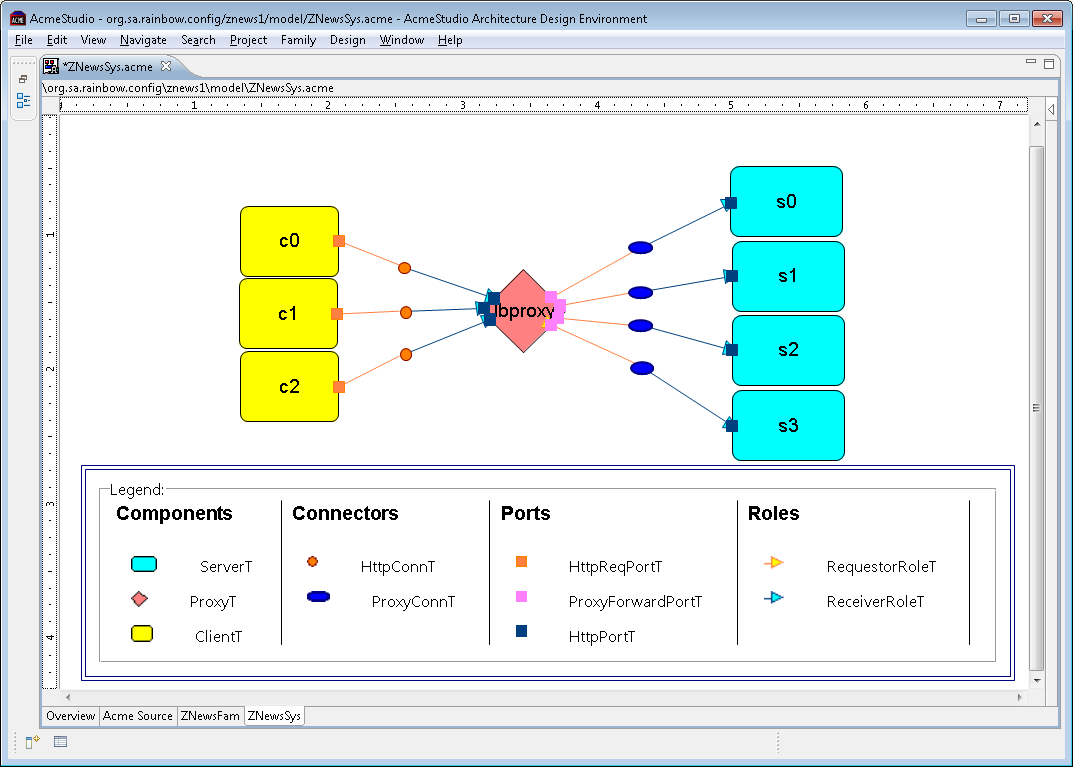
\includegraphics[width=0.82\textwidth]{images/znnArchitecture.png}
			\caption{Arquitectura de Znn vista en Acme Studio}
			\label{fig:znnArchitecture}
		\end{figure}

		En la arquitectura de Znn est�n definidos tres \emph{concerns} aunque en el presente trabajo, a saber:

		\begin{itemize}
			\item \textbf{Tiempo de Respuesta}: tiempo de respuesta promedio experimentado por el usuario de Znn, y
			\item \textbf{Costo}: el cual, refleja la cantidad de servidores prestando servicio con los que Znn cuenta en un
			determinado momento.
			\item \textbf{Fidelidad del Contenido}: trata sobre la \textbf{calidad} del contenido ofrecido por un servidor de
			Znn. A fin de mejorar el \emph{throughput}, un servidor podr�a servir contenido en un modo \emph{full} (texto,
			videos, audio, animaciones, etc.), en un modo s�lo texto o bien en una combinaci�n de estos dos.
		\end{itemize}

		Para las pruebas realizadas en este trabajo, s�lo se utilizar�n las siguientes t�cticas, con el fin de modificar el
		comportamiento del sistema en ejecuci�n:
		\begin{itemize}
			\item Dar de alta un servidor
			\item Dar de baja un servidor
			\item Disminu�r la fidelidad del contenido provisto por un servidor.
		\end{itemize}

		Para que estas t�cticas puedan ejecutarse, Znn implementa los correspondientes \emph{effectors}, quienes ser�n
		los responsables de efectuar los cambios propiamente dichos sobre el sistema en \emph{runtime}. Los \emph{effectors}
		ser�n invocados desde las t�cticas, cuyas implementaciones en Znn pueden verse en el ap�ndice \ref{sec:tacticasZNN}.
	
	\subsection{Configuraci�n B�sica para Casos de Prueba}
	\label{sec:configBasicaCasosPrueba}
	
		Como parte de la configuraci�n utilizada para las pruebas que ser�n presentadas en esta secci�n, es necesario definir
		los siguientes conceptos:

		\begin{itemize}
		  \item Entorno de carga normal.
		  \item Entorno de alta carga.
		  \item Escenario de tiempo de respuesta experimentado por el usuario.
		  \item Escenario de costo de servidores del sistema.
		  \item Estrategias asociadas a cada escenario, las cuales ser�n presentadas a medida que su utilizaci�n sea
		  requerida.
		\end{itemize}
		
		\begin{figure}[H]
			\centering
				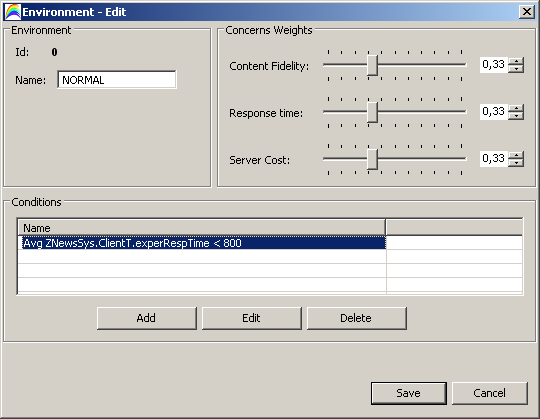
\includegraphics[scale=0.6]{images/Environment_Normal.png}
			\caption{Entorno de ejecuci�n de carga normal}
			\label{fig:Environment_Normal}
		\end{figure}

		Cabe destacar que para el entorno de carga normal, la configuraci�n por defecto de los pesos para cada uno de los
		\emph{concerns} del sistema se encuentra equidistribuida. Esta decisi�n convierte a las prioridades entre
		escenarios, cuando todos ellos pertenecen al entorno de carga normal, en el �nico factor influyente en la selecci�n de
		una estrategia candidata para reparar el sistema (ver algoritmo de selecci�n de estrategias en la secci�n
		\ref{sec:arcoIrisStrategyScoring}), simplificando as� los c�lculos, as� como tambi�n la comprensibilidad de los
		resultados presentados.

		\begin{figure}[H]
			\centering
				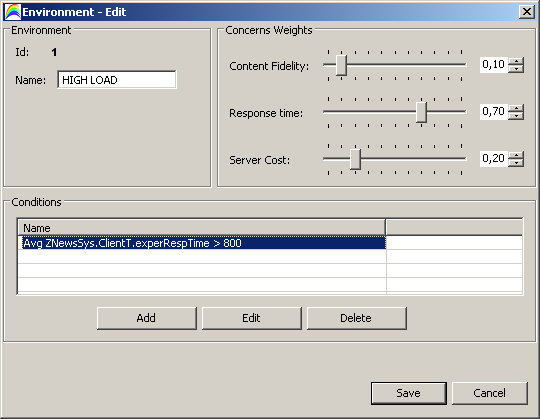
\includegraphics[scale=0.6]{images/Environment_HighLoad.png}
			\caption{Entorno de ejecuci�n de alta carga}
			\label{fig:Environment_HighLoad}
		\end{figure}

		En la figura \ref{fig:Environment_HighLoad} se puede observar la configuraci�n del entorno de alta carga, cuyos pesos
		no se encuentran equidistribu�dos, enfatizando as� la importancia del tiempo de respuesta frente a los restantes
		\emph{concerns} definidos en el sistema.
		
		\begin{figure}[ht]
			\centering
				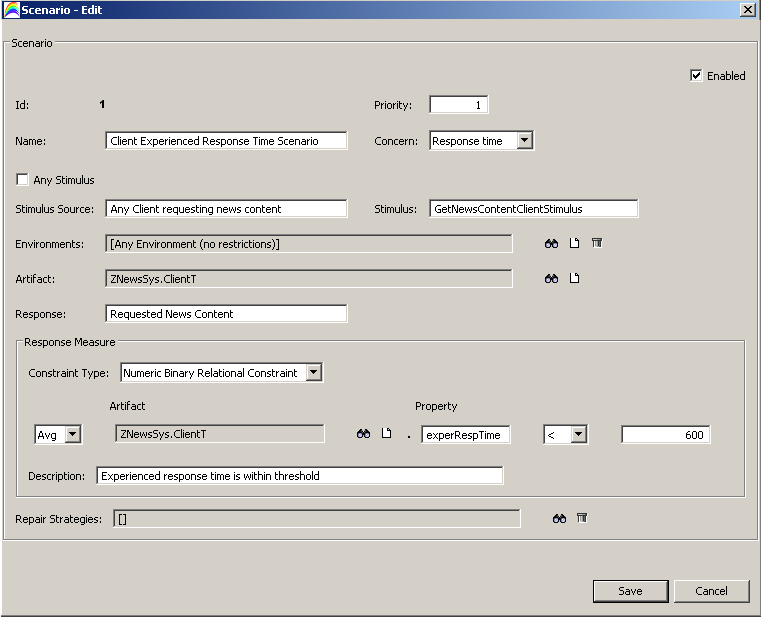
\includegraphics[width=0.8\textwidth]{images/scenario_expRespTime.png}
			\caption{Escenario de tiempo de respuesta experimentado por el usuario}
			\label{fig:scenario_expRespTime}
		\end{figure}

		\begin{figure}[H]
			\centering
				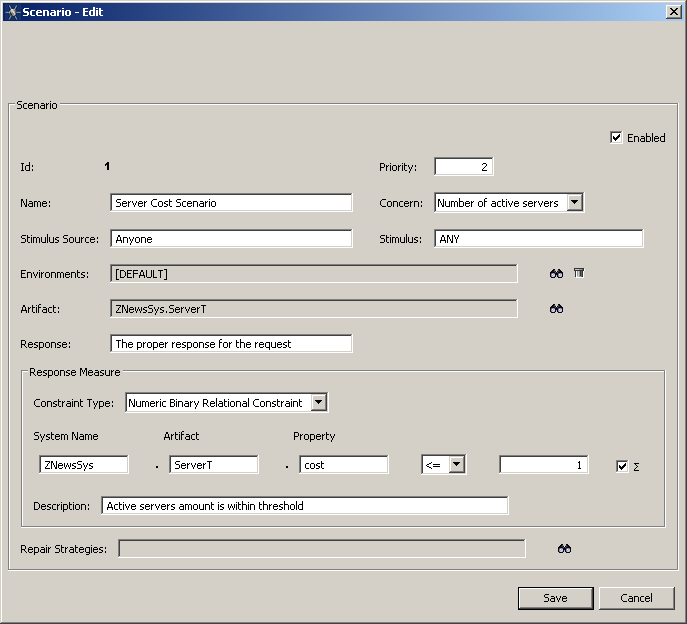
\includegraphics[width=0.8\textwidth]{images/scenario_cost.png}
			\caption{Escenario de costo de servidores del sistema}
			\label{fig:scenario_cost}
		\end{figure}

		En el ap�ndice \ref{sec:scenarioExpRespTimeXML} se muestra a modo de ejemplo la representaci�n en XML del escenario de
		tiempo de respuesta definido anteriormente.

		Con respecto a la configuraci�n por defecto de los escenarios aqu� definidos, notar lo siguiente:

		\begin{itemize}
			\item el escenario de tiempo de respuesta posee mayor prioridad que el de costo.
			\item ambos escenarios aplican para cualquier entorno en que se encuentre el sistema en ejecuci�n (ver definici�n del
			pseudo entorno ``ANY'' en la secci�n \ref{sec:environment});
			\item ambos escenarios no poseen estrategias de reparaci�n configuradas.
		\end{itemize}		
		
		La configuraci�n b�sica expuesta hasta aqu� ser� la utilizada por todos los casos de prueba a desarrollar en el
		presente trabajo. Al avanzar con las pruebas, y de acuerdo a las necesidades particulares de configuraci�n de cada
		una, ser� necesario efectuar algunos ajustes menores que impactar�n sobre los valores de los siguientes atributos:

		\begin{itemize}
		  \item Prioridad de cada escenario.
		  \item Estrategias asociadas a cada escenario.
		  \item Pesos de los \emph{concerns} para cada entorno.
		\end{itemize}

	\subsection{Caso 0: Comportamiento del Sistema sin Auto Reparaci�n}
		
		Para comenzar, se presenta el comportamiento del sistema de no existir escenarios ni estrategias, esto
		sentar� las bases para luego poder comparar y evaluar el comportamiento de Arco Iris a medida que se
		vayan agregando escenarios y/o estrategias en los siguientes casos de prueba a considerar.

		En la figura \ref{fig:Caso0} se puede observar el comportamiento del sistema sin escenarios, es decir, sin mecanismo
		de auto reparaci�n alguno.

		\begin{figure}[ht]
			\begin{center}
				\subfigure[Tiempo de Respuesta]{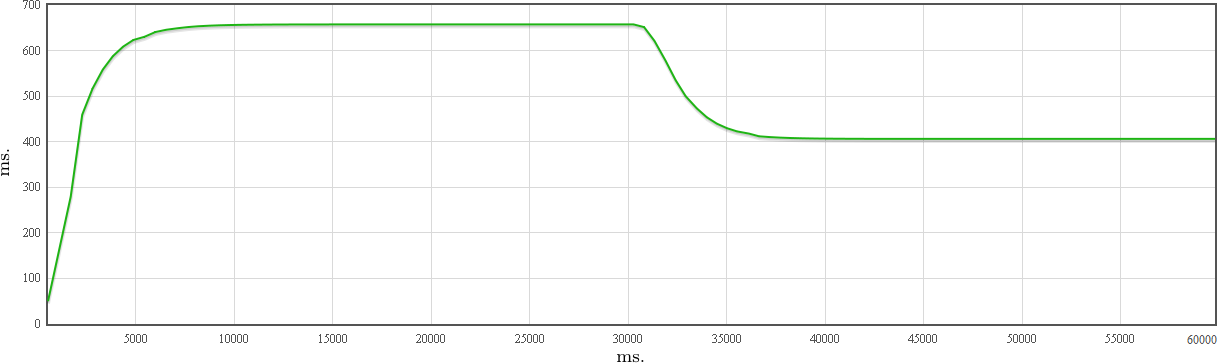
\includegraphics[width=\textwidth]{images/testcase0_expRespTime.png}}
				\subfigure[Costo de
				Servidores]{\label{fig:testcase0_cost}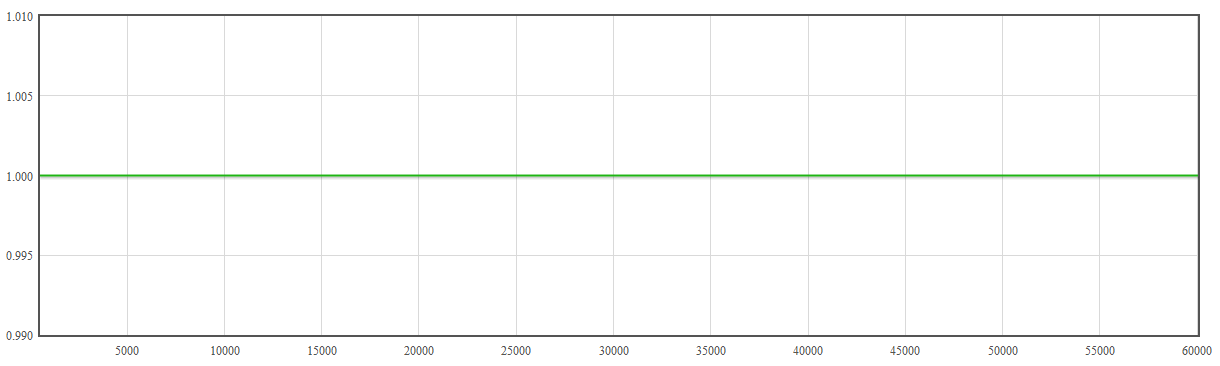
\includegraphics[width=\textwidth]{images/testcase0_cost.png}}
			\end{center}
			\caption{Comportamiento del sistema sin escenarios}
			\label{fig:Caso0}
		\end{figure}

		Como se puede observar, la simulaci�n ha sido configurada expl�citamente para que Znn se comporte de la siguiente
		manera: el tiempo de respuesta crece hasta superar los 600 ms., manteni�ndose all� hasta 30 segundos despu�s de haber
		comenzado la simulaci�n, para luego ir bajando paulatinamente hasta estacionarse cerca de los 400 ms. Notar que el
		costo de los servidores se mantiene inmutable frente a los cambios en el tiempo de respuesta, es decir que el sistema,
		de no mediar un usuario administrador o un \emph{framework} de auto reparaci�n como Arco Iris, trabaja siempre con un
		�nico servidor. Es importante tener en cuenta que la merma en el tiempo de respuesta no se debe a ninguna acci�n
		propia de la auto reparaci�n, sino a cambios en el ambiente, externos al sistema, como por ejemplo el ancho de banda
		de la conexi�n de cada uno de sus clientes.

	\subsection{Caso 1: Comportamiento con un Escenario, Sin Estrategias}

		Para el presente caso de prueba se utiliza el escenario de tiempo de respuesta definido anteriormente (ver figura
		\ref{fig:scenario_expRespTime}), el cual determina un umbral m�ximo aceptado de 600 ms. para el tiempo de respuesta
		experimentado por el usuario. 
		
		El objetivo de esta prueba es visualizar c�mo, al no haberse definido a�n ninguna estrategia, Arco Iris detectar� que
		existe un escenario que no se satisface aunque no efectuar� reparaci�n alguna sobre el sistema.

		Dado que Arco Iris no ejecuta estrategia alguna, el costo de servidores no se ver� modificado, manteni�ndose constante
		en 1, tal como se ha visto en la figura \ref{fig:testcase0_cost}.
		
		Por otro lado, en la figura \ref{fig:testcase1_expRespTime} se puede observar que Arco Iris detecta que, a partir de
		cierto instante, el tiempo de respuesta alcanza y supera el umbral predefinido en la cuantificaci�n de la respuesta
		del �nico escenario del sistema.
		
		\begin{figure}[ht]
			\centering
				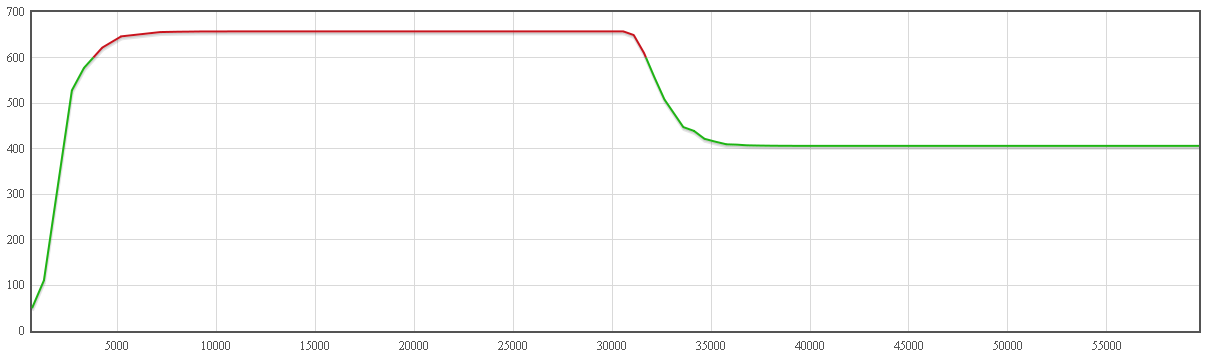
\includegraphics[width=1.00\textwidth]{images/testcase1_expRespTime.png}
			\caption{El umbral definido para el tiempo de respuesta es superado}
			\label{fig:testcase1_expRespTime}
		\end{figure}

	\subsection{Caso 2: Comportamiento con un Escenario y una Estrategia}
	\label{sec:testCase2}

		En el presente caso se intenta reflejar c�mo Arco Iris repara el sistema al encontrar una estrategia candidata adecuada
		para el escenario de tiempo de respuesta anteriormente presentado. Para tal fin, se define una estrategia que consiste
		simplemente en agregar un servidor, siempre y cuando existan servidores disponibles. La estrategia, definida en Stitch,
		posee la siguiente l�gica:

		\begin{Verbatim}[gobble=3]
			strategy EnlistServerResponseTime {
			  t0: (true) -> enlistServers(1) @[5000 /*ms*/] {
			    t1: (!RESP_TIME_STILL_BROKEN) -> done;
			    t2: (default) -> TNULL;
			  }
			}
		\end{Verbatim}

		Al agregar esta estrategia al escenario, se observa en la figura \ref{fig:testcase2_expRespTime} que el tiempo de
		respuesta experimentado por el usuario mejora (i.e. desciende) r�pidamente. De manera simult�nea a esta mejora, el
		costo de servidores aumenta a 2, producto de la ejecuci�n de la estrategia. Esto puede observarse en la figura
		\ref{fig:testcase2_cost}.

		\begin{figure}[ht]
			\begin{center}
				\subfigure[Mejora en el tiempo de respuesta debido a la ejecuci�n de una
				estrategia]{\label{fig:testcase2_expRespTime}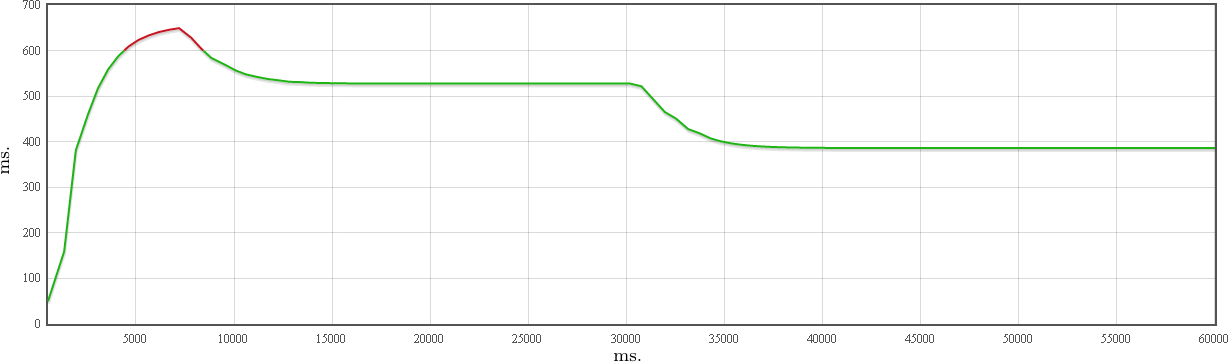
\includegraphics[width=1.00\textwidth]{images/testcase2_expRespTime.png}}
				\subfigure[Impacto de la estrategia sobre el costo de
				servidores]{\label{fig:testcase2_cost}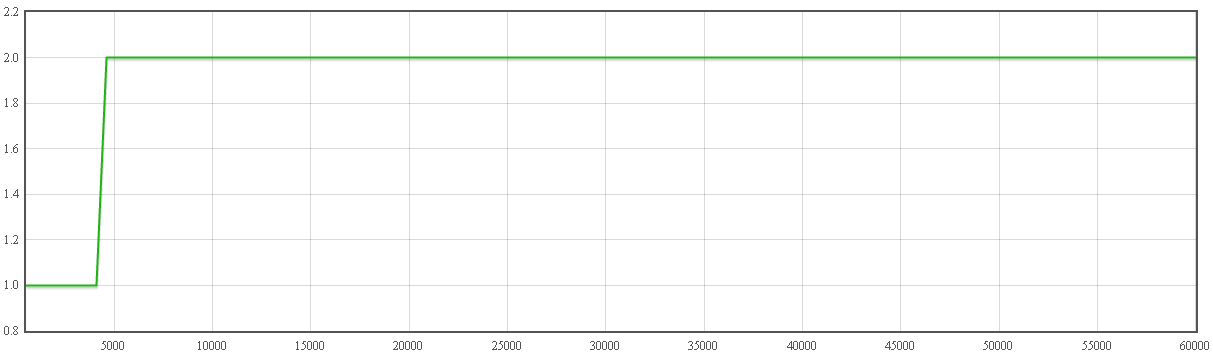
\includegraphics[width=1.00\textwidth]{images/testcase2_cost.png}}
			\end{center}
			\caption{Impacto del agregado de una estrategia}
			\label{fig:Caso2}
		\end{figure}

		En resumen, se ha visto hasta aqu� el comportamiento del sistema en las siguientes circunstancias:
		\begin{enumerate}
			\item no existe informaci�n alguna sobre auto reparaci�n.
			\item se ha definido un escenario pero sin estrategias que lo puedan reparar.
			\item se ha definido un escenario con una estrategia asociada.
		\end{enumerate}

		Antes de proseguir con casos de prueba m�s complejos, cabe mencionar que los \emph{logs} generados por Arco Iris
		ofrecen la informaci�n necesaria para analizar en detalle los casos de pruebas presentados en este informe. Dada la
		extensi�n de dichos archivos, es inviable mostrarlos todos para cada caso de prueba, por lo cual, a modo de ejemplo,
		en el ap�ndice \ref{sec:logCasoPruebaArcoIris} se presenta un extracto del \emph{log} generado por Arco Iris para el
		caso que se acaba de desarrollar en esta secci�n.

	\subsection{Caso 3: \emph{Tradeoff} entre Estrategias}
	
		El presente caso intenta mostrar c�mo Arco Iris escoge, entre varias estrategias candidatas para un mismo escenario,
		aquella que maximiza la utilidad del sistema.
		
		En particular, este caso presenta dos escenarios: uno relacionado con el costo de servidores, sin estrategias de
		reparaci�n definidas; y otro cuyo \emph{concern} es el tiempo de respuesta, configurado con la estrategia
		\verb@EnlistServerResponseTime@ antes definida y la introducci�n de una nueva estrategia:
		
		\begin{Verbatim}[gobble=3]
			strategy LowerFidelityReduceResponseTime {
			  t0: (true) -> lowerFidelity(2, 100) @[5000 /*ms*/] {
			    t1: (!RESP_TIME_STILL_BROKEN) -> done;
			    t2: (RESP_TIME_STILL_BROKEN) -> lowerFidelity(2, 100) @[8000 /*ms*/] {
			      t2a: (!RESP_TIME_STILL_BROKEN) -> done;
			      t2b: (default) -> TNULL;  // in this case, we have no more steps to take
			    }
			  }
			}
		\end{Verbatim}

		En concreto, en este caso de prueba se puede observar de qu� manera (mediante el uso del concepto de
		\textbf{Utilidad del Sistema}), Arco Iris - dentro de las estrategias que reparan al escenario en cuesti�n - otorga
		m�s valor a aquellas estrategias que no ``rompen'' otro escenario, es decir, las que dejan al sistema en una situaci�n
		m�s estable.
		
		Es de notar que, al ``competir'' estrategias relacionadas con el mismo \emph{concern} y reparando ellas al mismo
		escenario, las prioridades configuradas para cada escenario, en este caso, carecen de importancia.
		
		Cabe mencionar que, para que el escenario de costo deje de cumplirse, debe ser un escenario que aplique al entorno
		actual del sistema. Esta condici�n se satisface trivialmente, considerando que el escenario de costo fue definido para
		aplicar en cualquier entorno.
		
		En el siguiente extracto de \emph{log} se puede observar c�mo Arco Iris considera las estrategias mencionadas,
		escogiendo a \verb@LowerFidelityReduceResponseTime@ por sobre\\
		\verb@EnlistServerResponseTime@, ya que si bien ambas reparan al escenario de tiempo de respuesta, la �ltima rompe al
		escenario de costo de servidores:
		
		\begin{Verbatim}[gobble=3]
			...
			Evaluating strategy EnlistServerResponseTime...
			Scoring EnlistServerResponseTime...
			  Server Cost Scenario broken after simulation for Server Cost ([ESum] 2.0)? true
			  Experienced Response Time Scenario broken after simulation for Response time ([EAvg] 457.81)? false
			  Score for strategy EnlistServerResponseTime: 0.333
			  Current best strategy EnlistServerResponseTime
			  Evaluating strategy LowerFidelityReduceResponseTime...
			Scoring LowerFidelityReduceResponseTime...
			  Server Cost Scenario broken after simulation for Server Cost ([ESum] 1.0)? false
			  Experienced Response Time Scenario broken after simulation for Response time ([EAvg] 481.81)? false
			  Score for strategy LowerFidelityReduceResponseTime: 0.49
			  Current best strategy: LowerFidelityReduceResponseTime
			Selected strategy!: LowerFidelityReduceResponseTime
			EXECUTING STRATEGY LowerFidelityReduceResponseTime...
			...
		\end{Verbatim}
		
		Por �ltimo, en la figura \ref{fig:Caso3} se pueden observar las variaciones de los \emph{concerns} tiempo de
		respuesta, costo de servidores y fidelidad, para este caso de prueba. 
		
		\begin{figure}[H]
			\begin{center}
				\subfigure[Reparaci�n del tiempo de respuesta usando la mejor estrategia]
						  {\label{fig:testcase3_expRespTime}
						  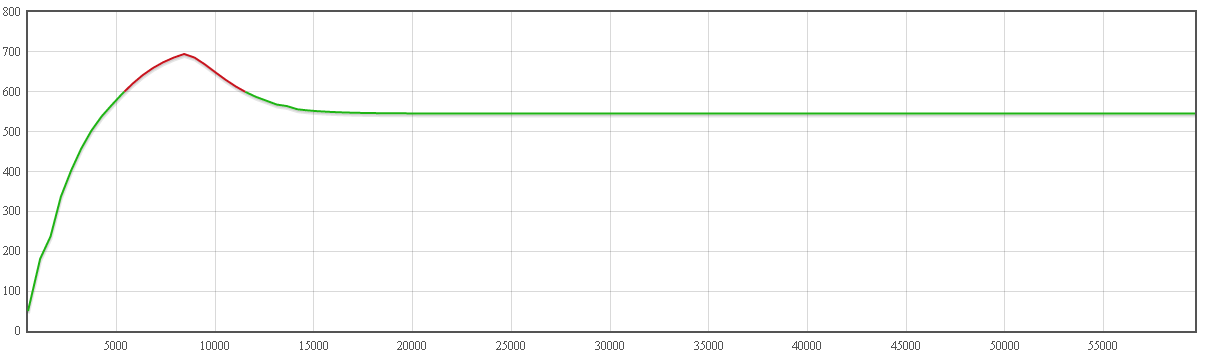
\includegraphics[width=0.99\textwidth]{images/testcase3_expRespTime.png}}
				\subfigure[El costo de servidores se mantiene intacto]
						  {\label{fig:testcase3_cost}
						  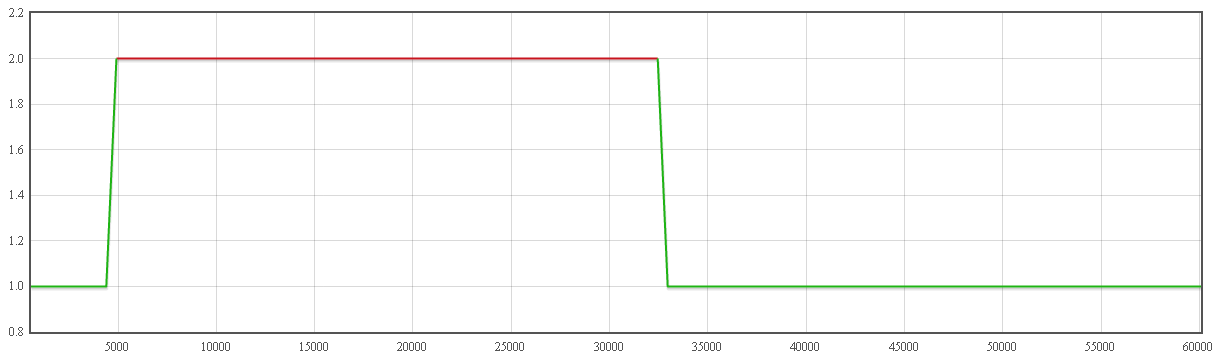
\includegraphics[width=0.99\textwidth]{images/testcase3_cost.png}}
				\subfigure[Desciende la fidelidad de la informaci�n]
						  {\label{fig:testcase3_fidelity}
						  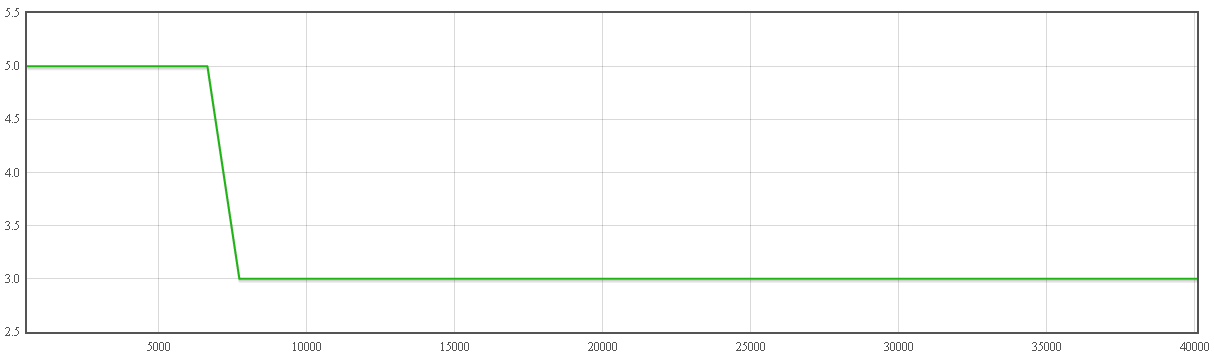
\includegraphics[width=0.99\textwidth]{images/testcase3_fidelity.png}}
			\end{center}
			\caption{Variaciones de los tres \emph{concerns} involucrados}
			\label{fig:Caso3}
		\end{figure}
		
	\subsection{Caso 4: \emph{Tradeoff} entre Escenarios seg�n Prioridades}

		El objetivo de esta prueba consiste en evaluar el comportamiento de Arco Iris ante la existencia de escenarios con
		distintas prioridades.

		Para el presente caso de prueba, se toma como base la configuraci�n del caso anterior con las siguientes
		modificaciones:
		\begin{itemize}
			\item El escenario de tiempo de respuesta contar� ahora solamente con la estrategia\\
			\verb@EnlistServerResponseTime@,
			\item Al escenario de costo se le agrega una estrategia de reparaci�n, cuya l�gica puede verse a continuaci�n:

			\begin{Verbatim}[gobble=4]
				strategy ReduceOverallCost {
				  t0: (true) -> dischargeServers(1) @[2000 /*ms*/] {
				    t1: (!COST_STILL_BROKEN) -> done;
				    t3: (default) -> TNULL;
				  }
				}
			\end{Verbatim}
		\end{itemize}

		Como ya se ha mencionado en la introducci�n de la presente secci�n (ver secci�n \ref{sec:configBasicaCasosPrueba}), el
		escenario de tiempo de respuesta es m�s prioritario que el de costo. Esta configuraci�n es crucial en este caso de
		prueba, ya que determinar� el rumbo de la auto reparaci�n llevada a cabo por Arco Iris.

		En las figuras \ref{fig:testcase4_expRespTime} y \ref{fig:testcase4_cost} se puede observar el comportamiento del
		tiempo de respuesta y del costo, respectivamente, para la configuraci�n actual.

		\begin{figure}[H]
			\begin{center}
				\subfigure[Uso de prioridades favoreciendo al escenario de eficiencia por sobre el de costo]
						  {\label{fig:testcase4_expRespTime}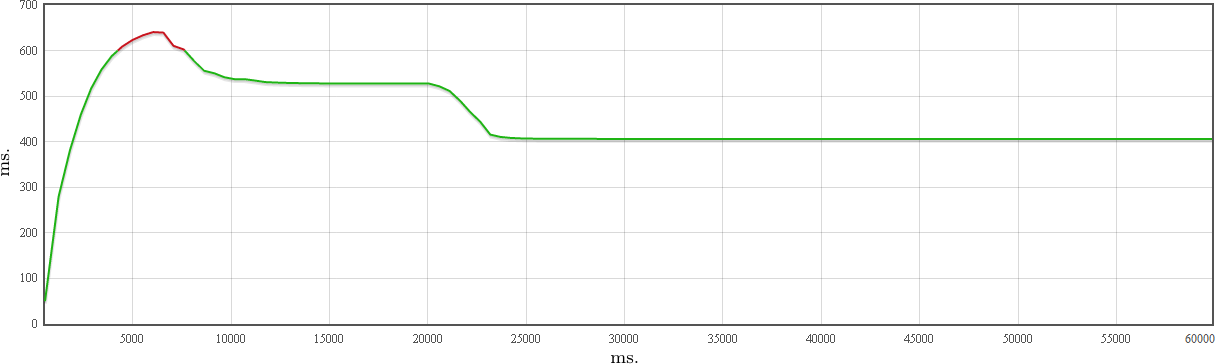
\includegraphics[width=1.00\textwidth]{images/testcase4_expRespTime.png}}
				\subfigure[Reducci�n del costo como consecuencia de un cambio en el entorno]
						  {\label{fig:testcase4_cost}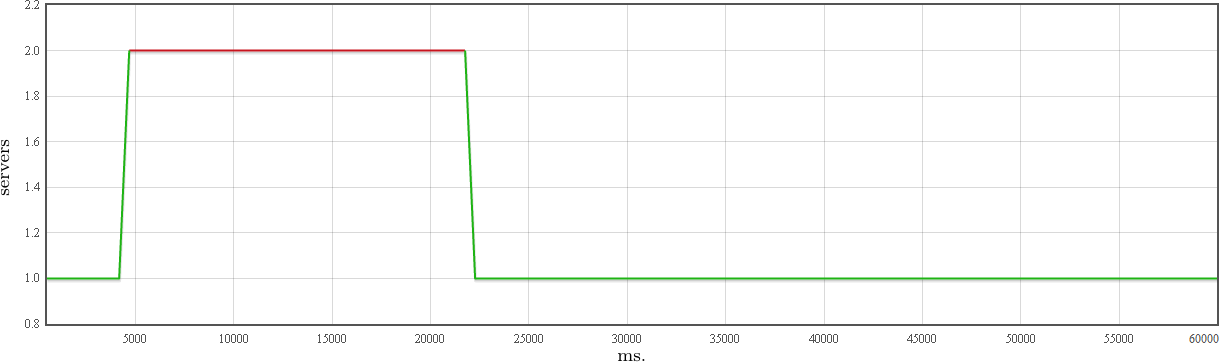
\includegraphics[width=1.00\textwidth]{images/testcase4_cost.png}}
			\end{center}
			\caption{Comportamiento del sistema respetando prioridades entre escenarios}
			\label{fig:Caso4}
		\end{figure}

		Tal cual se ha visto en los casos b�sicos anteriores, el escenario de tiempo de respuesta es el primero en dejar de
		cumplirse. Considerando que s�lo se ha configurado una �nica estrategia de reparaci�n para dicho escenario, la misma
		es ejecutada exitosamente, ya que cerca de los 9 segundos, el tiempo de respuesta vuelve a ubicarse en valores aceptables.
		
		Ahora bien, la estrategia ejecutada consiste ni m�s ni menos que en agregar un servidor m�s al sistema, con lo cual se
		observa en la figura \ref{fig:testcase3_cost} de qu� manera, a partir de los 5 segundos, el escenario relacionado con
		el costo de servidores deja de cumplirse, puesto que la cantidad m�xima de servidores all� especificados es 1.
		
		Arco Iris debe decidir si repara o no a este nuevo escenario que se ha ``roto''. Es aqu� d�nde las prioridades entre
		escenarios juegan un papel determinante: dado que el escenario relaciondo con el tiempo de respuesta es m�s
		prioritario que aqu�l relacionado con el costo de servidores, Arco Iris decide no efectuar reparaci�n alguna sobre
		este �ltimo, ya que detecta (mediante la heur�stica explicada en la secci�n \ref{sec:arcoIrisStrategyScoring}) que el
		arreglar el escenario de costo, potencialmente llevar�a a ``romper'' el escenario de tiempo de respuesta, que es m�s
		prioritario. En otras palabras, la auto reparaci�n provista por Arco Iris no intentar� reparar el escenario de costo
		de servidores mientras que la utilidad del sistema en el estado actual sea mayor a la prevista en caso de repararlo.

		En la figura \ref{fig:testcase3_cost}, aproximadamente a partir de los 33 segundos, se puede observar c�mo Arco Iris
		decide desactivar un servidor en el preciso momento en que el entorno de ejecuci�n de la aplicaci�n cambia y el
		tiempo de respuesta mejora por razones ajenas a la auto reparaci�n. Aprovechando esto, Arco Iris logra satisfacer as�
		al escenario que estaba sin cumplirse, sin perjudicar al otro escenario (m�s prioritario) que se estaba cumpliendo
		hasta ese momento.

		Finalmente, se arriba a un estado de estabilidad d�nde ambos escenarios se satisfacen simult�neamente. Si bien el tiempo
		de respuesta sufre un peque�o detrimento al trabajar el sistema con un servidor menos, los valores de las
		propiedades relacionadas con los \emph{concerns} de inter�s, siguen siendo lo suficientemente aceptables como para no
		violar ninguna de las restricciones definidas en la cuantificaci�n de la respuesta de los escenarios aqu�
		configurados.
		
		En resumen, se ha mostrado por un lado la potencia y conveniencia de agregar el concepto de prioridad entre escenarios
		como un elemento de relevancia para configurar al \emph{framework} y por otro, c�mo distintos escenarios con
		distinta prioridad pueden convivir en Arco Iris, tomando �ste decisiones inteligentemente sobre qu� escenario(s)
		reparar, considerando siempre como factor crucial, la utilidad que el sistema exhibir�a de ejecutar, o no, determinada
		estrategia de reparaci�n.

	\subsection{Caso 5: \emph{Tradeoff} entre Escenarios seg�n \emph{Concerns}}

		El objetivo de este caso de prueba es analizar c�mo Arco Iris, al tener que escoger entre favorecer dos escenarios
		con igual prioridad, elige favorecer a aquel cuyo \emph{concern} posee un peso mayor para el entorno de ejecuci�n
		actual.

		Los escenarios utilizados en este caso de prueba son id�nticos a los del caso anterior, excepto que ahora pasan a
		tener ambos igual prioridad y el escenario de costo no posee estrategias de reparaci�n asociadas. Por otro lado, el
		entorno de carga normal pasa a asignar mayor peso al \emph{concern} costo de servidores:
		
		\begin{figure}[H]
			\centering
				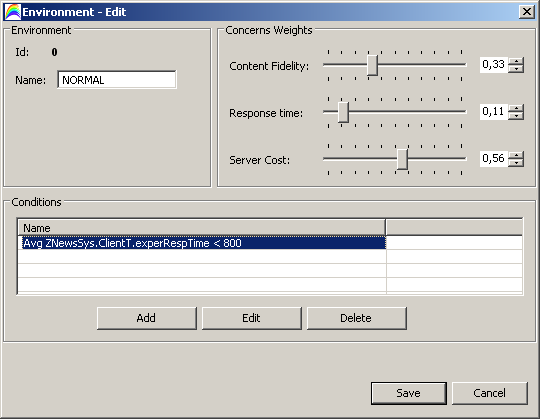
\includegraphics[scale=0.6]{images/testcase5_normal_environment_modified.png}
			\caption{Nueva distribuci�n de pesos para el entorno ``normal''}
			\label{fig:testcase5_normal_environment_modified}
		\end{figure}

		En el extracto del \emph{log} generado por Arco Iris se observa c�mo, al igual que en la mayor�a de los casos de
		pruebas ya presentados aqu�, el escenario de tiempo de respuesta deja de cumplirse y Arco Iris debe decidir qu�
		acci�n llevar a cabo ante dicha situaci�n. Puede apreciarse que Arco Iris opta por no reparar el escenario de tiempo de
		respuesta ya que esto perjudicar�a al escenario de costo, puesto que si bien ambos poseen id�ntica prioridad, el
		�ltimo est� relacionado al \emph{concern} \textbf{costo de servidores}, el cu�l en el entorno de ejecuci�n actual
		(normal) tiene m�s peso que el \emph{concern} \textbf{tiempo de respuesta}.
		
		En otras palabras, al igual que en el caso anterior, Arco Iris vuelve a utilizar la Utilidad del sistema como una
		medida para estimar el estado en que quedar�a el sistema, de ejecutar o no una determinada estrategia; concluyendo
		que, en el caso de intentar reparar el escenario de tiempo de respuesta ``roto'', el sistema brindar�a menos utilidad
		que en el estado actual. Vale reiterar que el factor determinante en el c�lculo de dicha utilidad simulada del sistema
		es, ni m�s ni menos, que el peso del \emph{concern} costo de servidores posee en el entorno de ejecuci�n actual.

		\begin{Verbatim}[gobble=3]
			Current environment: NORMAL
			Computing Current System Utility...
			Server Cost Scenario broken for [ESum] 1.0? false
			Experienced Response Time Scenario broken for [EAvg] 602.25? true
			Current System Utility (Score to improve): 0.555
			Evaluating strategy EnlistServerResponseTime...
			  Scoring EnlistServerResponseTime...
			  Server Cost Scenario broken after simulation for Server Cost ([ESum] 2.0)? true
			  Experienced Response Time Scenario broken after simulation for Response time ([EAvg] 458.25)? false
			  Score for strategy EnlistServerResponseTime: 0.111
			NO applicable strategy, adaptation cycle ended.
		\end{Verbatim}
		
		Cabe mencionar que, avanzada ya la ejecuci�n del sistema, el tiempo de respuesta vuelve a estar por debajo del umbral
		m�ximo definido en el escenario correspondiente. Esto, nuevamente, se debe a condiciones cambiantes en el entorno de
		ejecuci�n y no a una acci�n activa llevada a cabo por el \emph{framework} para lograr tal efecto. Esta situaci�n,
		junto con las variaciones del tiempo de respuesta durante toda la ejecuci�n de este caso de prueba, pueden
		visualizarse en la figura siguiente:
		
		\begin{figure}[H]
			\centering
				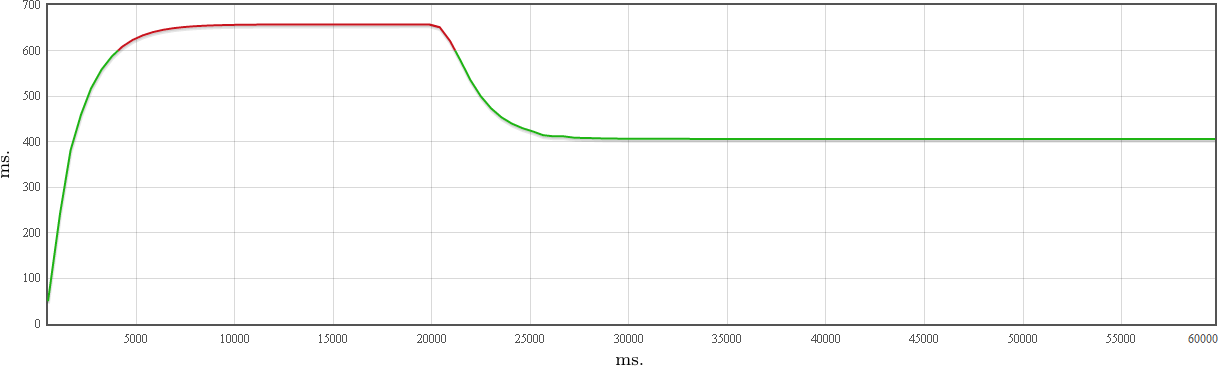
\includegraphics[width=1.00\textwidth]{images/testcase5_expRespTime.png}
			\caption{El tiempo de respuesta no es reparado por Arco Iris, arreglandose s�lo luego.}
			\label{fig:testcase5_expRespTime}
		\end{figure}

		Cabe destacar que el costo de servidores, por su parte, se mantiene constante en 1 durante toda la ejecuci�n.

	\subsection{Caso 6: Comportamiento Ante Los Cambios en el Entorno de Ejecuci�n}

		Este caso de prueba pretende demostrar c�mo Arco Iris var�a su comportamiento dependiendo del entorno en el cual se
		encuentra ejecutando el sistema en un momento dado.
	
		Para este caso es necesario contar con tres escenarios similares a los utilizados hasta aqu� pero con las siguientes
		variaciones:
		\begin{itemize}
		  \item Un escenario de \textbf{prioridad 3} cuya cuantificaci�n de la respuesta acota el tiempo de respuesta a 600
		  ms. como m�ximo, cuando el sistema se encuentra en \textbf{carga normal}.
		  \item Un escenario de \textbf{prioridad 1} que define que el tiempo de respuesta no debe superar los 900 ms. cuando
		  el sistema se encuentra bajo \textbf{alta carga}.
		  \item Un escenario de \textbf{prioridad 2} que predica sobre el costo de servidores, \textbf{limitando al sistema a
		  utilizar como m�ximo un servidor}, cuando se encuentre en un entorno de \textbf{carga normal}.
		\end{itemize}
		
		En otras palabras, mientras el sistema se encuentre dentro de par�metros normales de carga (i.e. carga normal), se
		prefiere que el tiempo de respuesta suba por encima de su umbral m�ximo (600 ms.) antes que agregar un servidor m�s
		al sistema. Ahora, cuando el entorno de ejecuci�n es de alta carga, el tiempo de respuesta pasa a tener m�s
		importancia que el costo de servidores. Esto, en teor�a, habilitar�a a Arco Iris a agregar uno o m�s servidores en pos
		de que el tiempo de respuesta no supere su umbral m�ximo (900 ms.) para un entorno de alta carga. Este es el objetivo
		primordial de este caso de prueba.
		
		Para lograr que el sistema en un momento determinado de la ejecuci�n pase a estar en alta carga, ha sido necesario
		modificar los par�metros de la simulaci�n, generando as� condiciones que emulan un incremento en la carga de pedidos
		al �nico servidor disponible en el sistema. Recordar que la condici�n que especifica cu�ndo el sistema se encuentra en
		alta carga, est� configurada en el entorno definido en la secci�n \ref{sec:configBasicaCasosPrueba} (ver figura
		\ref{fig:Environment_HighLoad}).
		
		Los escenarios de tiempo de respuesta tendr�n asociada la estrategia de auto reparaci�n
		\verb@EnlistServerResponseTime@, utilizada en pruebas anteriores, mientras que el escenario de costo no poseer�
		estrategias asociadas.
		
		Tal como se esperaba, Arco Iris no toma acci�n alguna mientras el sistema se encuentra en carga normal, puesto que el
		escenario de costo posee m�s prioridad que el escenario de tiempo de respuesta para dicho entorno. Esto se puede
		apreciar en la figura \ref{fig:testcase6_expRespTime}.

		\begin{figure}[ht]
			\begin{center}
				\subfigure[Arco Iris s�lo arregla el tiempo de respuesta con el sistema en alta carga.]
						  {\label{fig:testcase6_expRespTime}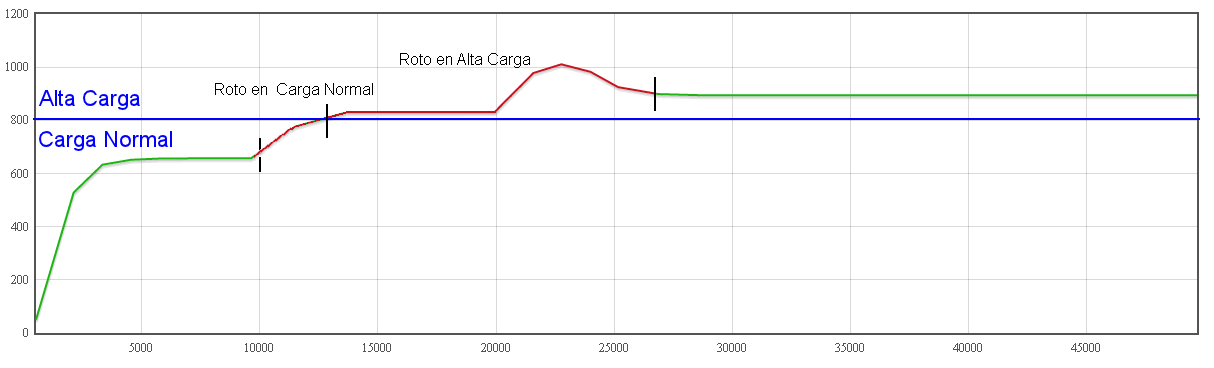
\includegraphics[width=\textwidth]{images/testcase6_expRespTime.png}}
				\subfigure[En carga normal, el costo es priorizado y se mantiene en 1.]
						  {\label{fig:testcase6_cost}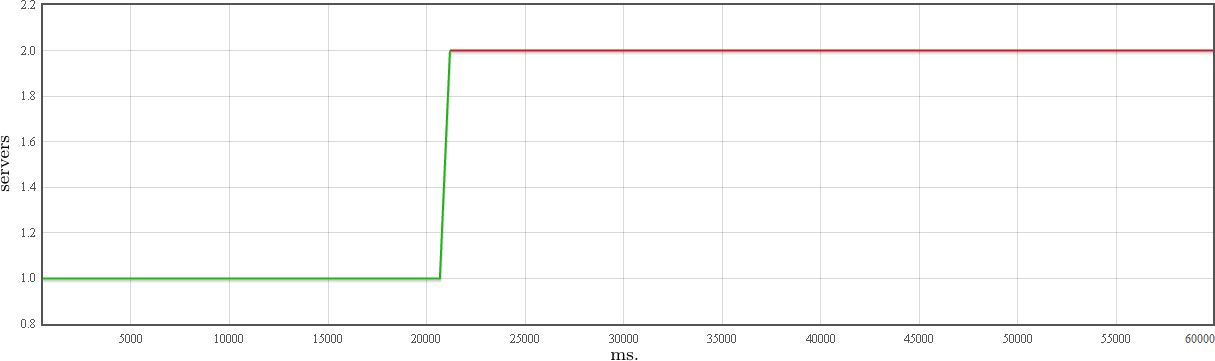
\includegraphics[width=\textwidth]{images/testcase6_cost.png}}
			\end{center}
			\caption{Comportamiento del sistema en distintos entornos de ejecuci�n}
			\label{fig:Caso6}
		\end{figure}
		
		Luego de superados los 800 ms. el sistema pasa a estar en alta carga, por lo cual dos de los tres escenarios pasan a
		satisfacerse trivialmente. Consecuentemente, Arco Iris deber� procurar s�lamente que se cumpla el escenario de tiempo
		de respuesta que impide que se superen los 900 ms. Puede observarse en la figura \ref{fig:testcase6_cost} que la auto
		reparaci�n decide agregar un servidor aproximadamente a partir de los 23 segundos de iniciada la simulaci�n, reparando
		efectivamente el escenario en cuesti�n.
		
		% \todo{no deber�amos tener que poner tener que poner este clearpage ac�\ldots} 
		\clearpage

\newpage

\section{Trabajo Futuro}

	\todo{C�mo seleccionar la mejor estrategia. Lo del ``utility function'' es limitado.
	- C�mo incluir algo de aprendizaje sobre el resultado de las reparaciones anteriores (m�s sofisticado, lo que hay
	ahora es muy limitado)
	- Mi idea original de usar para algo los ``artifacts'' vinculados al escenario
	- Expandir la idea del ``system environment'' (tenemos una implementaci�n muy restrictiva, no se pueden solapar e.g.
	alta carga y super alta carga (a.k.a. hasta las tetas) ).
	- No alcanza con la UI (y su XML asociado) para configurar 100\% nuestra soluci�n (hace falta configurar cosas por
	fuera)}

	Desde ya se entiende que el presente trabajo deja abiertas muchas posibilidades de mejoras que ser�n necesarias al
	momento de implementar este framework como una herramienta de uso generalizado en la industria, a continuaci�n
	citaremos las m�s importantes desde nuestro punto de vista.

	\subsection{An�lisis y Aprendizaje de la Auto Reparaci�n}

		Supongamos que los \emph{stakeholders} ya han definido todos los escenarios que se utilizar�n en la reparaci�n via
		Arco Iris. Ahora bien, imaginemos que existe un escenario cuya prioridad es muy alta y a su vez las condiciones
		necesarias para que el mismo se rompa se dan con mucha frecuencia. Esto resultar� en la auto reparaci�n repetida del
		mencionado escenario. Pero �qu� suceder�a si la �nica que estrategia que repara dicho escenario rompe constantemente
		otros, digamos 3 escenarios de menor prioridad? A priori pareciera que este es el comportamiento esperado, pero
		�podr�an los \emph{stakeholders} convalidar este comportamiento? Claramente se necesitan una serie de estad�sticas que
		nos permitan analizar lo que se est� reparando, y el impacto sobre los escenarios perjudicados, y tambi�n ser�a
		necesaria una vista sobre el impacto en cada uno de los \emph{concerns} del sistema.

		Por otro lado, supongamos que bajo la misma situaci�n, la �nica estrategia que aplica para reparar el escenario falla
		en un 95\% de los casos, �tiene sentido continuar ejecutando dicha estrategia teniendo en cuenta c�mo afecta la
		performance del sistema y de la auto reparaci�n? Una soluci�n sencilla ser�a permitirle definir al usuario un umbral
		de	fallos, por ejemplo definiendo que si una estrategia falla el 90\% de los intentos o m�s, la misma queda eliminada
		de	las estrategias candidatas.

		Si bien lo menciona en el �ltimo p�rrafo se encuentra implementado, consideramos que la implementaci�n es bastante
		b�sica y poco flexible. Por ejemplo ser�a �til que antes de llegado a ese punto, se notifique, a modo de alarma, al
		responsable de la auto reparaci�n de que una estrategia a estado fallando. Podr�an existir sucesivas alarmas antes de
		desactivar la estrategia. Tambi�n deber�a permitirse modificar din�micamente tanto la l�gica de la estrategia como las
		condiciones esperadas en el escenario.

		Tambi�n ser�a �til proveer una herramienta que permita analizar que estrategias se fueron ejecutando, y c�mo se lleg�
		a decidir que cada estrategia era la adecuada para reparar el sistema en cada momento. Otra vista que ser�a �til para
		analizar la configuraci�n de la auto reparaci�n del sistema podr�a ser un \emph{ranking} de estrategias, en el que	se
		presente el porcentaje de �xito de cada una as� como la cantidad de veces que se ejecut�, como qued� el \emph{Utility
		Function} en promedio luego de ejecutar la estrategia, etc.

		\todo{JONY: se te ocurre algo mas sobre el aprendizaje sobre el resultado de las reparaciones anteriores???}

	\subsection{Configuraci�n Din�mica}

		Cuando se desarrolla un sistema se hacen presunciones y supuestos, asumiendo determinados comportamiento que
		indefectiblemente variar�n cuando el sistema se est� ejecutando: errores del sistema, cambios en el entorno (variaci�n
		de recursos), cambios en las preferencias del usuario, etc. El reconocimiento de dichas presunciones es muy importante
		ya que esto acercar� al sistema al ``mundo real'', y ser�n muy importantes a la hora de reparar el sistema, y m�s a�n
		si se desea implementar un mecanismo de auto reparaci�n flexible y din�mico.

		Dicho esto, se propone como trabajo a futuro dinamizar la configuraci�n de auto reparaci�n de Arco Iris, permitiendo
		que los \emph{stakeholders} modifiquen los escenarios en caliente, es decir, sin necesidad de detener el framework.
		Esto es importante ya que de requerir un sistema alta disponibilidad, no podr� darse el lujo de que el mecanismo de
		auto reparaci�n que utilice sea detenido para reconfigurarlo, sino que debe adaptarse a las nuevas condiciones
		pr�cticamente sin \emph{impasse}.

	\subsection{Configuraci�n de Escenarios en AcmeStudio}

		Actualmente existe una herramienta de creaci�n y edici�n de arquitecturas modeladas en Acme, llamado AcmeStudio
		\cite{AcmeStudio} la cual se encuentra integrada en la popular herramienta de desarrollo Eclipse\cite{Eclipse} como un
		\emph{plug-in}.

		Se propone como trabajo a futuro extender la herramienta AcmeStudio para que d� soporte a las extensiones propuestas
		en el presente trabajo, permitiendo as� la integraci�n del modelado de la arquitectura con el modelado de los
		escenarios que la complementan, utilizando la misma herramienta.

	\subsection{Optimizaci�n en la Selecci�n de la Estrategia}

		\todo{Se deja para el final: c�mo seleccionar la mejor estrategia (Lo del ``utility function'' es limitado)}

	\subsection{\todo{Puntas sueltas:}}

		\begin{itemize}
			\item Mi idea original de usar para algo los ``artifacts'' vinculados al escenario
			\item Expandir la idea del ``system environment'' (tenemos una implementaci�n muy restrictiva, no se pueden solapar
			e.g. alta carga y super alta carga).
			\item No alcanza con la UI (y su XML asociado) para configurar 100\% nuestra soluci�n (hace falta configurar cosas
			por fuera). Por ejemplo: usamos la tablita de las utility functions.
			\item{Ni Rainbow bi Arco Iris permiten cambair en runtime la configuracion}
			\item{Permitir agregar concerns nuevos}
			\item{leer los artifacts y sus properties desde el .ACME}
			\item{agregar mas tipos de constraints}
		\end{itemize}


\newpage

\section{Conclusiones}

	\subsection{Objetivo}

		El presente trabajo permite a los sistemas que implementen Arco Iris \textbf{contar con la definiciones de sus
		requerimientos de atributos de calidad}, en lugar de simplemente poseer implementaciones de posibles soluciones a los
		mismos. No es menor el hecho de que estas definiciones est�n al alcance de todos \emph{stakeholders} participantes,
		cambio radical con respecto al enfoque planteado por Rainbow.

		Este conocimiento es fundamental para lograr el objetivo de esta tesis, que consiste en permitir ampliar el estudio de
		los sistemas aut�nomos introduciendo un modelo flexible de auto reparaci�n basado en la arquitectura de los sistemas,
		ya que adem�s de poner sobre el tablero los requerimientos, los hace visibles a todo el conjunto de participantes del
		desarrollo. De esto se desprende directamente el hecho de que los sistemas podr�n poseer un espectro m�s amplio de
		soluciones, las cu�les ser�n seleccionadas seg�n los requerimientos vayan modific�ndose como consecuencia de
		variaciones en el entorno de ejecuci�n bajo el cual el sistema deba responder. Este dinamismo en la reparaci�n, as�
		como tambi�n la flexibilidad en el modelo de selecci�n de soluciones y su f�cil configuraci�n, hacen de Arco Iris una
		opci�n plausible a ser considerada y extendida para lograr avanzar en la flexibilizaci�n de sistemas inteligentes, a
		la vez que permite incorporar cada vez m�s la utilizaci�n de la auto reparaci�n en la industria del software.

	\subsection{Resumen del trabajo realizado}

		En resumidas palabras, el presente trabajo a�ade una serie de caracter�sticas a Rainbow, todas ellas tendientes a
		disponer de una herramienta gen�rica de auto reparaci�n m�s poderosa y flexible y que, al mismo tiempo, los actores
		funcionales del sistema se vean involucrados en el proceso de definici�n de requerimientos de atributos de calidad,
		puesto que este tipo de actores son los encargados de determinar (junto a arquitectos, dise�adores, etc.) c�mo se debe
		comportar el sistema ante determinadas situaciones de operaci�n. Las caracter�sticas a�adidas en este trabajo son
		b�sicamente las siguientes:
		\begin{itemize}
			\item Posibilidad de modelar escenarios de atributos de calidad siguiendo los principios de ATAM y QAW.
			\item Posibilidad de relacionar escenarios con componentes de la arquitectura.
			\item Posibilidad de especificar prioridades relativas entre escenarios, a ser utilizadas en la elecci�n de la
			estrategia de reparaci�n a ejecutar.
			\item Definici�n de entornos de ejecuci�n para el sistema, con ponderaciones particulares para cada uno
			de los \emph{concerns} existentes, los cuales juegan un papel determinante en el algoritmo de elecci�n de
			estrategias de reparaci�n.
			\item Posibilidad de asociar estrategias de reparaci�n a escenarios.
			\item Modelado de un nuevo algoritmo de elecci�n de la mejor estrategia, utilizando todos los conceptos
			introducidos en Arco Iris.
			\item Implementaci�n de cambios en diversos m�dulos de Rainbow (como por ejemplo, el \emph{RainbowModel} y el
			\emph{AdaptationManager} e implementaci�n de algunos casos pr�cticos que permitan mostrar c�mo esta estrategia
			puede funcionar y llevar a un \emph{framework} de adaptaci�n m�s flexible y poderoso.
			\item Implementaci�n de un mecanismo de recarga din�mica de la configuraci�n de Arco Iris, la cu�l en un futuro
			podr�a ser f�cilmente integrada a Rainbow en pos de dinamizar el uso del \emph{framework}, minimizando su
			\emph{downtime} debido a cambios en la configuraci�n.
			\item Implementaci�n de una herramienta visual de escritorio que permita al usuario de Arco Iris, configurar el
			\emph{framework} de una manera sencilla, amena y eficiente.
		\end{itemize}

		Todo lo antedicho tiene como consecuencia que los usuarios tendr�n m�s herramientas para influir sobre lo que el
		sistema decida hacer para auto repararse: s�lo con modificar la informaci�n de los escenarios el sistema modificar� su
		comportamiento. Como contrapartida, las extensiones propuestas en este trabajo hacen que el sistema se comporte de
		manera m�s aut�noma a medida que se agregan escenarios; esto parad�jicamente le quita control al usuario, ya que el
		procedimiento de auto reparaci�n se vuelve m�s complejo, dificultando el seguimiento de las decisiones tomadas por el
		\emph{framework}.

	\subsection{Arco Iris comparado con Rainbow}

		\noindent En la presente secci�n repasaremos las ventajas que posee Arco Iris por sobre Rainbow. Profundizaremos en
		los siguientes puntos b�sicos:

		\noindent \todo{sacar grafico y poner tabla cuando imprimamos la versi�n definitiva (es para evitar falsos bad boxes)}
%  		\begin{center}
%  			\scriptsize{
%  			\rowcolors*[\hline]{1}{GreenYellow!25}{GreenYellow!10}
%  			\begin{tabularx}{\textwidth}{|X|X|X|X|}
%   			\textbf{Problema} & \textbf{Implementaci�n en Rainbow} & \textbf{Implementaci�n en \mbox{Arco Iris}} &
%   			\textbf{Ventajas}\\
%   			Rapidez en el cambio de configuraci�n & La configuraci�n se lee una vez al principio y no puede ser cambiada
%   			din�micamente mientras Rainbow est� funcionando. & Los escenarios se actualizan din�micamente en \emph{runtime} al
%   			ser modificados. & Una gran parte de los cambios de configuraci�n pasan a impactarse ins\-tan\-t�\-nea\-men\-te,
%   			evitando reiniciar el sistema para cambiar la configuraci�n\\
%   			Informaci�n sobre restricciones & Guardadas en el modelo de la arquitectura (en \mbox{ACME}) & Mediante escenarios
%   			de QAW editados por \emph{stakeholders} & F�cil y transparente agregado y edici�n de las mismas.\\
%   			Decisiones sobre que reparaciones realizar & Tambi�n se encuentran en archivos de configuraci�n & Se evalu�n los
%   			escenarios cargados y como se afectan entre ellos. Luego se invoca a un m�dulo que decide qu� reparaciones pueden
%   			llevarse a cabo en ese contexto. & Posibilidad de extensi�n de dicho m�dulo para inclu�r complejas heur�sticas que
%   			aprendan de los efectos de reparaciones pasadas, etc.\\
%   			Entorno de ejecuci�n (e.g. Alta Carga)& Configurado est�ticamente. Para modificarlo es necesario el reinicio del
%   			\emph{framework}. & Se permite especificar distintos entornos de ejecuci�n. El sistema cambia
%   			di\-n�\-mi\-ca\-men\-te de en\-tor\-no sin necesidad de in\-ter\-ven\-ci�n humana ni reinicio del \emph{framework}.
%   			& Se agrega una nueva variable a considerar para la elecci�n de una estrategia, aumentando la probabilidad de que
%   			la misma se adeque mejor a la situaci�n actual del sistema.
%  			\end{tabularx}
%  			}
%  		\end{center}
			
		\begin{center}
			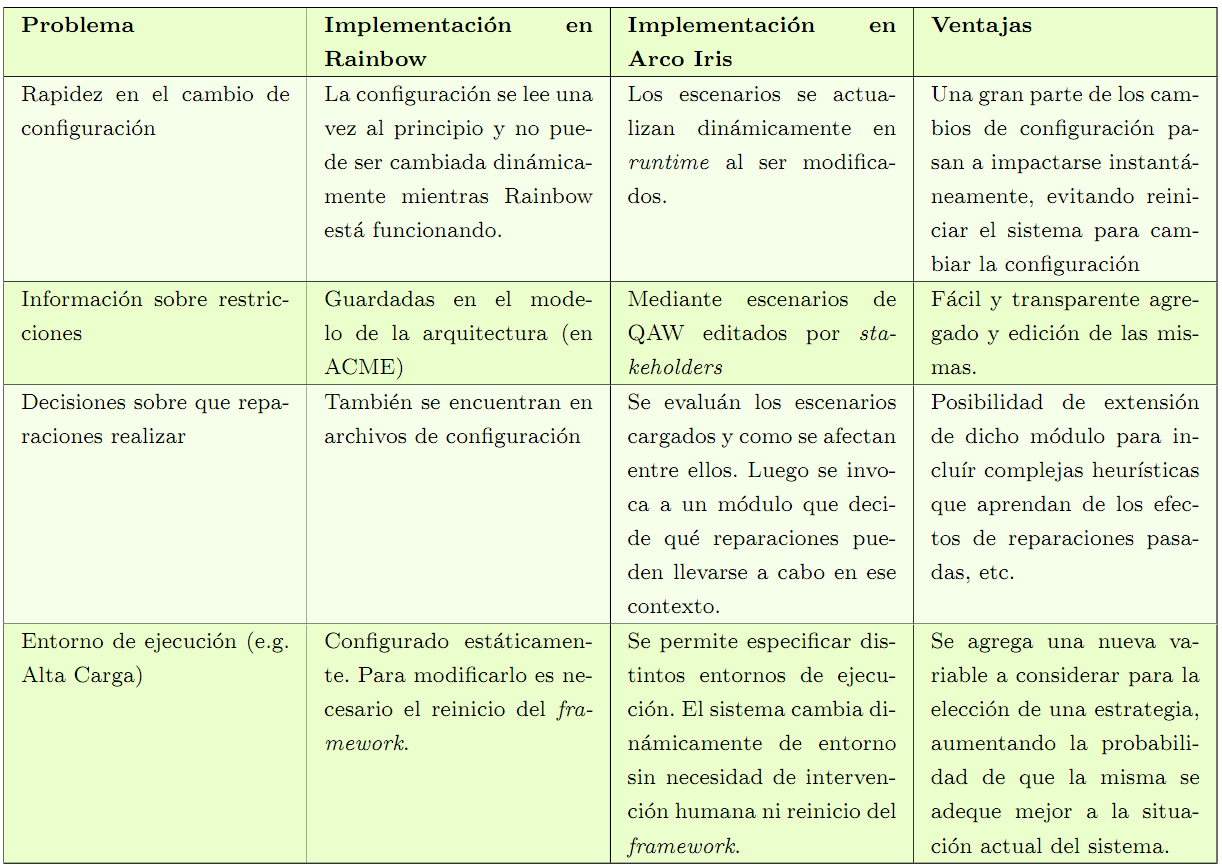
\includegraphics[width=1.00\textwidth]{images/ArcoIrisVsRainbow.png}
		\end{center}

		\subsubsection{Rapidez en el cambio de configuraci�n}
		
			Como se ha mencionado anteriormente, Arco Iris (es decir, Rainbow con las extensiones realizadas en este trabajo)
			trabaja utilizando:
			\begin{itemize}
				\item por un lado, una configuraci�n de \emph{Self Healing} en formato XML, producida ya sea por la herramientas
				Arco Iris UI o bien manualmente; la cual incluye: escenarios de QAW, entornos de ejecuci�n y \emph{artifacts}.
				\item por otro, una bater�a de archivos de configuraci�n heredados de Rainbow, en distintos formatos: stitch, ACME,
				\emph{properties files}, etc.
			\end{itemize}
			Una de las mejoras que agrega este trabajo a Rainbow es el de proveer un mecanismo din�mico de actualizaci�n de la
			configuraci�n de \emph{Self Healing} mediante el cual cualquier modificaci�n en el archivo XML de configuraci�n
			cargada al iniciar Arco Iris, conlleva un ``refresco'' de la configuraci�n que est� siendo usada en tiempo de
			ejecuci�n por el \emph{framework}, sin necesidad de intervenci�n alguna de un operador.
			
			Este dinamismo agregado en lo que respecta a los cambios de configuraci�n, trae aparejado una considerable serie de
			ventajas, a saber:
			\begin{itemize}
				\item ya no es necesario reiniciar el \emph{framework} de auto reparaci�n para modificar cualquier caracter�stica
				relacionada con los escenarios, entornos de ejecuci�n y \emph{artifacts} utilizados en el sistema. Esto evita
				tiempos de no-servicio, recursos involucrados en la reconfiguraci�n y reinicio del sistema, etc. 
				\item se agrega flexibilidad al uso de la herramienta: se podr�an agregar nuevos escenarios, nuevos entornos de
				ejecuci�n que (re)definan situaciones de ejecuci�n concretas, cambiar pesos de \emph{concerns} y/o prioridades relativas
				entre escenarios de acuerdo a necesidades puntuales del negocio e infinidad de otros cambios de configuraci�n
				relevantes a la auto reparaci�n quedar�an impactados en el sistema autom�ticamente.
			\end{itemize}
			
		\subsubsection{Informaci�n sobre restricciones}
		
			Como se ha visto anteriormente, en Rainbow las restricciones impuestas sobre el funcionamiento del sistema (e.g.
			``el tiempo de respuesta para cualquier tipo de \emph{request} no debe superar los 5 m�lisegundos'') son guardadas en
			el modelo de la arquitectura, el cual est� expresado en el lenguaje de descripci�n de arquitecturas \mbox{ACME}.
			Esto claramente representa un impedimento para que los \emph{stakeholders} no t�cnicos puedan participar activamente
			en la definici�n de requerimientos de auto reparaci�n del sistema; ya que de intentarlo, deber�an poder comprender y
			modificar correctamente un diagrama de arquitectura, con sus restricciones escritas en un lenguaje no coloquial sino
			especialmente t�cnico.
			
			En Arco Iris, los \emph{stakeholders} usan una interfaz visual\ref{sec:arcoIrisUI} intuitiva y f�cil de utilizar
			para expresar restricciones del sistema en formato de escenarios de QAW; los cuales a su vez fueron pensados
			originalmente para facilitar la participaci�n de personas con roles funcionales.
			
			La informaci�n incorporada de esta manera, es analizada por Arco Iris para tomar decisiones en tiempo de ejecuci�n
			sobre las auto reparaciones a realizar, considerando una variedad de aspectos, todos ellos configurados en un �nico
			lugar: los escenarios de QAW.
			
			Como vemos, Arco Iris provee una manera simplificada de agregar y/o editar restricciones sobre el sistema, sin
			necesidad de modificar su modelo de arquitectura, sino por medio de los escenarios de QAW. Esto representa una avance
			sobre como funciona Rainbow hoy d�a en ese aspecto.

		\subsubsection{Decisiones sobre que reparaciones realizar}

			Con respecto a este punto, la diferencia principal entre Rainbow y Arco Iris es el enfoque: al momento de
			decidir qu� estrategia es la m�s adecuada para ser ejecutada en el contexto de una o m�s \emph{constraints} no
			cumpliendose, en Rainbow se calcula un \emph{score} para cada una de las estrategias existentes en el sistema,
			mientras Arco Iris busca aquellos escenarios de QAW ``rotos'' y s�lo asigna un \emph{score} a las estrategias
			definidas en dicho subconjunto de escenarios. Este enfoque, adem�s de ser m�s eficiente, es considerablemente mas
			sencillo de configurar y tiene m�s sentido a nivel funcional, ya que en el caso de Rainbow no parece haber una manera
			sencilla de intu�r de antemano qu� estrategia eligir�a en cada caso, hecho que complica en an�lisis de las
			reparaciones efectuadas por Rainbow durante el transcurso de una ejecuci�n.

		\subsubsection{Entorno de ejecuci�n}

			En Rainbow, el concepto de entorno de ejecuci�n es est�ticamente configurado en un archivo de configuraci�n y no se
			modifica de acuerdo al estado din�mico del sistema que se intenta reparar. Para modificar tal est�tico y limitado valor, es
			necesario el reinicio de Rainbow.
			
			El modelo de Arco Iris incluye el concepto de Entorno de Ejecuci�n tal cual es descripto en la
			metodolog�a ATAM\cite{ATAM}, el cual permite al usuario especificar distintos entornos de ejecuci�n posibles para el
			sistema, los cuales poseen restricciones asociadas que se chequean continuamente y que, de cumplirse, hacen que se
			considere que el sistema se encuentra en otro entorno de ejecuci�n, afectando as� al algoritmo de decisi�n de
			estrategias de reparaci�n; ya que dicha decisi�n est� condicionada al \emph{scoring} de estrategias de reparaci�n, el
			cual se realiza considerando los pesos relativos que poseen los \emph{concerns} arquitecturales en el entorno de ejecuci�n
			actual.
			
			Lo antedicho, agrega una nueva arista a las variables consideradas al momento de elegir la mejor estrategia de
			reparaci�n, aumentando las probabilidades de que la estrategia seleccionada sea m�s precisa de acuerdo a la situaci�n
			del sistema en tiempo de ejecuci�n.
			
			Si bien en Rainbow el concepto de ``entorno de ejecuci�n'' no existe como tal, uno podr�a encontrarlo indirectamente
			dentro de ciertas condiciones de aplicabilidad embebidas dentro del c�digo de las estrategias de reparaci�n.
			
			Ahora bien, observemos que Rainbow no tiene forma de determinar a priori si alguna de las estrategias configuradas
			por el usuario van a aplicar en el contexto actual de ejecuci�n: dada alguna \emph{constraint} violada, necesita
			inspeccionar la totalidad de las estrategias para verificar si son aplicables en la situaci�n actual de
			\emph{runtime}. Esto �ltimo es una notable diferencia a favor de Arco Iris, ya que en este caso, al estar las
			estrategias de reparaci�n candidatas embebidas en el escenario, aquellos escenarios cuyo entorno no se corresponda
			con el entorno actual de ejecuci�n, no se considerar�n ``rotos'', evitando c�mputos innecesarios y refinando
			as� el m�todo original provisto por Rainbow.

	\subsection{Compatibilidad hacia atr�s: una empresa sin sentido}

		Uno de los objetivos de dise�o m�s deseables en una extensi�n a un \emph{framework} ya existente como Rainbow, es sin
		dudas que la extensi�n sea ``compatible hacia atr�s'' con \emph{Rainbow}, entendiendose �sto como la capacidad de
		Arco Iris de agregar nuevas caracter�sticas manteniendo al 100\% la funcionalidad original. 
		
		En principio, si se considera �nicamente el dise�o de alto nivel de Rainbow, la idea de una extensi�n \emph{backwards
		compatible} parece factible. Pero, lamentablemente, si se consideran las diferencias conceptuales de ambos modelos,
		no es dif�cil notar que el intento de mantener a ambos conviviendo no s�lo no es una tarea sencilla sino que tambi�n
		carece de sentido, ya que, en algunos puntos claves, son enfoques diametralmente opuestos. Veamos algunos de los
		motivos que apoyan esta idea:
		
		\begin{itemize}
			\item \textbf{C�mo se dispara la auto reparaci�n:} El enfoque de Arco Iris hace centro en el concepto de Escenario
			como medio para expresar requerimientos de atributos de calidad para un sistema. Con lo cual, el inicio de todo el
			proceso de auto reparaci�n se da de una manera sincr�nica con respecto al Est�mulo de alg�n escenario(s) ocurrido en
			el sistema en ejecuci�n. Esto se contrapone con el enfoque de Rainbow, en el cual, peri�dicamente se verifican todas
			las restricciones e invariantes de la arquitectura. Observamos que si quisieramos mantener esta �ltima
			caracter�stica de Rainbow, ya el foco absoluto de la auto reparaci�n no estar�a puesto en los Escenarios de
			atributos de calidad sino que paralelamente existir�an dos flujos distintos de auto reparaci�n disputando entre s�.
			Esto llevar�a a un comportamiento excesivamente complejo y poco predecible, lo cual resulta poco deseable para un
			\emph{framework} de auto reparaci�n.
			\item \textbf{C�mo se decide cu�ndo adaptar:} Arco Iris s�lo intenta efectuar adaptaciones acotadas al escenario o
			los escenarios que se dejan de cumplir en un determinado momento, mientras que Rainbow contempla todo el abanico de
			estrategias disponibles en el caso de que detecte que una violaci�n a una restricci�n o invariante ha tenido lugar.
			Evidentemente, los enfoques son distintos, sin mencionar que los algoritmos de \emph{scoring} de estrategias de
			ambos \emph{frameworks} difieren considerablemente, agregando el algoritmo de Arco Iris nuevas variables a la
			f�rmula, tal como se explica en la secci�n \ref{sec:arcoIrisStrategyScoring}.
		\end{itemize}

	\subsection{Aplicabilidad en sistemas reales}

		Luego de haber repasado las caracter�sticas principales de Arco Iris y de haber entendido su mec�nica, es muy probable
		que al lector se le suscite la siguiente pregunta: �Qu� aplicabilidad tiene esta extensi�n de Rainbow en un	sistema real?
		
		Consideramos que Arco Iris se encuentra un paso m�s cerca de ser utilizado en un sistema de \emph{software} real (i.e.
		en un �mbito no acad�mico) que lo que su antecesor, Rainbow, se encontraba. Esta consideraci�n se basa en el hecho de
		que Arco Iris hace foco en la accesibilidad del usuario final para configurar el \emph{framework} de una manera amena
		y m�s flexible que la provista originalmente por Rainbow, incluyendo una interfaz de usuario visual que facilita dicha
		tarea as� tambi�n como el mantenimiento y evoluci�n de configuraci�n existente.
		
		Habiendo dicho lo anterior, tambi�n reconocemos que Arco Iris todav�a puede no ser la herramienta m�s s�lida y madura
		que los sistemas de \emph{software} de la industria necesitan para confiar la compleja y crucial tarea de agregar auto
		reparaci�n a un sistema. Esto tiene como causas diversos motivos, algunos de los m�s importantes son:
		
		\begin{itemize}
			\item Actualmente, no todas las organizaciones que desarrollan \emph{software} poseen un modelo formal de la
			arquitectura, tal como es requerido por Rainbow o Arco Iris. Esto forma parte de una tendencia por parte de La
			industria del \emph{software} a desarrollar sistemas, a veces de envergadura y de misi�n cr�tica, de una manera
			todav�a artesanal. Esta realidad complica la adopci�n de \emph{frameworks} que centren la auto reparaci�n de un
			sistema en el modelo de su arquitectura. Sin embargo, como hemos mencionado en la secci�n
			\ref{sec:ausenciaObsolescenciaModeloArquitectura}, existen l�neas de investigaci�n intentando atacar este problema,
			derivando el modelo de la arquitectura de un sistema a partir de informaci�n obtenida durante su ejecuci�n, lo cual
			representa un avance importante en pos de facilitar el uso de herramientas como Arco Iris.
			\item El trabajo de creaci�n de \emph{Gauges} y \emph{Probes} (los cuales usualmente no son reutilizables entre
			distintas aplicaciones) sigue siendo una tarea de complejidad no trivial a cargo del usuario del \emph{framework}.
			\item La informaci�n necesaria para que el \emph{framework} funcione, no obstante las mejoras introducidas en Arco
			Iris descritas en la secci�n \ref{sec:actualizacionDinamicaConfig}, sigue estando dispersa en diversos archivos de
			configuraci�n, en archivos separados de estrategias y t�cticas, en el modelo de la arquitectura, etc. Esto, sumado a
			una incompleta documentaci�n de Rainbow, configura una curva de aprendizaje del \emph{framework} un tanto pronunciada
			para un usuario nuevo. Es necesario seguir trabajando en la centralizaci�n de la configuraci�n (tal cual fue descrito
			en la secci�n \ref{sec:todaLaConfigEnUnSoloArchivo}) y tambi�n en el incremento de la documentaci�n para facilitar el
			uso, tanto de Rainbow como de Arco Iris.
		\end{itemize}


\newpage

\appendix
\clearpage
\addappheadtotoc
\appendixpage

\section{Instalaci�n y Ejecuci�n de Arco Iris y Arco Iris UI}
\label{sec:instalacionYEjecucionArcoIris}

	\todo{Revisar y actualizar todos los apendices}

	\subsection{Aclaraci�n importante}

		En el DVD que acompa�a al presente trabajo, se incluye el c�digo fuente de Rainbow, Arco Iris y Arco Iris UI, as�
		tambi�n como la totalidad de las herramientas necesarias para visualizar, compilar y ejecutar dichas aplicaciones. De
		cualquier manera, describiremos brevemente los requisitos y pasos necesarios para que cualquier persona interesada
		pueda instalar y ejecutar las aplicaciones producto  de este trabajo.

	\subsection{Prerrequisitos}
	\label{sec:prerrequisitos}

		\subsubsection{Requisitos para la Ejecuci�n de las Aplicaciones}

			\subsubsubsection{Java 6.0 o superior}

			Tanto Rainbow como Arco Iris y Arco Iris UI son aplicaciones Java que necesitan de una m�quina virtual Java instalada
			en la computadora d�nde se desee ejecutar estas aplicaciones. La misma se encuentra disponible para la gran
			mayor�a de las plataformas utilizadas com�nmente (Windows, Unix, Solaris, MAC OS, etc.) y puede ser descargada
			gratuitamente desde \url{http://www.oracle.com/technetwork/java/javase/downloads/index.html}.
			
			Luego de instalar la m�quina virtual de Java, es necesario configurar la variable de entorno \verb@JAVA_HOME@ para
			que apunte al directorio de instalaci�n. Ejemplos:
			
			\noindent En Windows:
			\begin{Verbatim}[gobble=4]			
				JAVA_HOME = %ProgramFiles%\Java\jdk1.6.0_23
			\end{Verbatim}

			\noindent En Linux:
			\begin{Verbatim}[gobble=4]			
				JAVA_HOME = /usr/lib/jvm/java-6-sun
			\end{Verbatim}

			Luego, es necesario que el ejecutable de Java se encuentre en el \emph{path} del sistema operativo. Para lograr esto,
			es necesario hacer lo siguiente:

			\noindent En Windows:
			\begin{Verbatim}[gobble=4]			
				PATH = %PATH%;%JAVA_HOME%\bin
			\end{Verbatim}
			
			\noindent En Linux:
			\begin{Verbatim}[gobble=4]			
				PATH = $PATH:$JAVA_HOME/bin
			\end{Verbatim}
			
			Para verificar que el ejecutable de Java va a poder ser utilizado normalmente, ejecutar el siguiente comando:
			
			\begin{Verbatim}[gobble=4]			
				> java -version
			\end{Verbatim} 
			
			\noindent Se deber�a obtener una respuesta de este tipo:

			\begin{Verbatim}[gobble=4]			
				java version "1.6.0_21"
				Java(TM) SE Runtime Environment (build 1.6.0_21-b06)
				Java HotSpot(TM) 64-Bit Server VM (build 17.0-b16, mixed mode)
			\end{Verbatim}
			
		\subsubsection{Requisitos para la Inspecci�n y Edici�n del C�digo Fuente}

			\subsubsubsection{Eclipse 3.6 o superior}

			En el caso en que se desee inspeccionar o editar el c�digo fuente de Rainbow, Arco Iris y/o Arco Iris UI, una
			herramienta no imprescindible aunque muy recomendada es \textbf{Eclipse}. Eclipse es un entorno de desarrollo
			integrado que permite visualizar, editar, compilar y ejecutar aplicaciones Java (entre muchas otras cosas). Se
			descarga gratuitamente desde \url{http://www.eclipse.org/downloads} y la versi�n ``for Java Developers'' es
			suficiente a los fines de trabajar con las aplicaciones que conciernen a este trabajo.
			
			El c�digo fuente inclu�do incluye metadatos de Eclipse, con lo cual, si se utilizan los correspondientes
			\emph{plugins} detallados a continuaci�n, deber�a ser relativamente sencillo poder disponer r�pidamente de todos
			los proyectos que conforman el tandem Rainbow-Arco Iris. los \emph{plugins} de Eclipse requeridos son:

			\begin{itemize}
				\item \textbf{Maven plugin}: El plugin para Eclipse de Maven. El mismo puede ser obtenido utilizando el
				\emph{Marketplace} de Eclipse o utilizando la siguiente URI
				\url{http://m2eclipse.sonatype.org/sites/m2e}.\footnote{Se presupone que el lector est� familiarizado con el
				mecanismo de instalaci�n de un \emph{plugin} de Eclipse, caso contrario, ver una explicaci�n en la siguiente p�gina
				web: \url{http://wiki.eclipse.org/FAQ_How_do_I_install_new_plug-ins\%3F}}
				\item \textbf{Subclipse}: Se trata del plugin para Eclipse que provee soporte para interactuar con repositorios
				Subversion\footnote{Para m�s informaci�n sobre Subversion, visitar \url{http://subversion.tigris.org/}}. Tanto
				el c�digo de Rainbow como el de Arco Iris se encuentran alojados en servidores Subversion (SVN).
			\end{itemize}

			\subsubsubsection{Maven 2 o superior}

			A fin de compilar y empaquetar el c�digo fuente de la aplicaci�n mediante la l�nea de comandos del sistema operativo,
			es necesario utilizar Maven, la popular herramienta de construcci�n de aplicaciones Java. Maven es una
			aplicaci�n multi plataforma con una abundante cantidad de documentaci�n de calidad, la cual puede ser consultada
			visitando su p�gina web: \url{http://maven.apache.org/}, desde la cual se pueden descargar tambi�n los binarios
			de dicha aplicaci�n.
			
			Para instalar Maven, basta con descomprimir el archivo \verb@.zip@ (o \verb@.tar.gz@) en un directorio a elecci�n y
			luego configurar la variables \verb@M2_HOME@ para que apunte a dicho directorio:

			\begin{Verbatim}[gobble=4]			
				M2_HOME = ~/apache-maven-3.0.3
			\end{Verbatim}

			Luego, es necesario que el ejecutable de Maven se encuentre en el \emph{path} del sistema operativo. Para ello, es
			necesario hacer lo siguiente:

			\begin{Verbatim}[gobble=4]			
				PATH = $PATH:$M2_HOME/bin
			\end{Verbatim}

			Para chequear si Maven va a poder ser utilizado normalmente, ejecutar el siguiente comando:
			
			\begin{Verbatim}[gobble=4]			
				> mvn --version
			\end{Verbatim} 
			
			\noindent Se deber�a obtener una respuesta de este tipo:

			\begin{Verbatim}[gobble=4]
				Apache Maven 3.0.3 (r1075438; 2011-02-28 14:31:09-0300)
				Maven home: ~/apache-maven-3.0.3
				Java version: 1.6.0_21, vendor: Sun Microsystems Inc.
				Java home: /usr/lib/jvm/java-6-sun-1.6.0.21/jre
				Default locale: en_US, platform encoding: UTF-8
				OS name: "linux", version: "2.6.38-8-generic", arch: "amd64", family: "unix"
			\end{Verbatim}

	\subsection{Obtenci�n del c�digo fuente de Rainbow, Arco Iris y Arco Iris UI}
	
		El grupo ABLE posee un repositorio SVN privado, el cu�l es s�lo accesible mediante el otorgamiento de un usuario
		(normalmente de s�lo lectura) con contrase�a, a pedido expl�cito del interesado. A fin de obtener dichas credenciales
		de acceso, es necesario redactar un e-mail a David Garlan $<$\url{garlan@cs.cmu.edu}$>$. Sin embargo, no es necesario
		obtener estas credenciales puesto que en el repositorio SVN de Arco Iris (\url{http://code.google.com/p/arco-iris}) se
		puede encontrar todo el c�digo necesario a los fines del presente trabajo.

		Tanto Arco Iris como Arco Iris UI son de c�digo abierto (\emph{open source}), esto significa que cualquier persona
		puede acceder libremente al c�digo fuente y examinarlo.

	\subsection{Estructura de Directorios del Presente Trabajo}

		A continuaci�n, se observa la estructura de directorios del c�digo fuente de las aplicaciones creadas/modificadas en
		el presente trabajo.
		
		\begin{figure}[h]
			\centering
				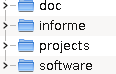
\includegraphics{images/directory_structure_root.png}
			\caption{Estructura de directorios de este trabajo}
		\end{figure}

 		\begin{center}
 			\begin{tabularx}{\textwidth}{p{3cm}X}
	  			\textbf{doc} & Aqu� se incluye un subconjunto de la bibliograf�a utilizada para la realizaci�n del presente
	  			trabajo, a modo de referencia r�pida en caso de estar leyendo el presente informe en forma digital.
	  		\end{tabularx}
	  		\begin{tabularx}{\textwidth}{p{3cm}X}
	  			\textbf{informe} & Incluye la propuesta de tesis y este documento en formato PDF.
	  		\end{tabularx}
	  		\begin{tabularx}{\textwidth}{p{3cm}X}
	  			\textbf{projects} & Aqu� se encuentra la totalidad del c�digo fuente correspondiente a las aplicaciones objeto de
	  			este trabajo: Arco Iris, Arco Iris UI, JFaceGUI (a continuaci�n, veremos de qu� se trata este proyecto) y algunos
	  			m�dulos de Rainbow que fueron ligeramente modificados. 
	  		\end{tabularx}
			\begin{tabularx}{\textwidth}{p{3cm}X}
				\textbf{software} & Aqu� se incluyen los prerequisitos para compilar y ejecutar las aplicaciones. (ver ap�ndice
				\ref{sec:prerrequisitos})
 			\end{tabularx}
 		\end{center}

		Hilando m�s fino en el directorio m�s importante de los anteriormente mencionados, observamos los proyectos contenidos
		en el directorio \verb@projects@:
		
		\begin{figure}[h]
			\centering
				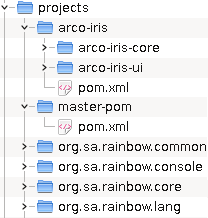
\includegraphics{images/directory_structure_projects.png}
				\caption{Estructura de directorios del directorio ``projects''}
		\end{figure}
		
		 \begin{center}
	  		\begin{tabularx}{\textwidth}{p{3cm}X}
	  			\textbf{arco-iris} & La totalidad del c�digo nuevo desarrollado para este trabajo, dividido en
	  			\verb@arco-iris-core@, Arco Iris propiamente dicho; y \verb@arco-iris-ui@.
	  		\end{tabularx}
			\begin{tabularx}{\textwidth}{p{3cm}X}
	  			\textbf{jFaceGUI} & En el desarrollo de una interfaz gr�fica para Arco Iris, se observ� la oportunidad de aislar
	  			un \emph{framework} gen�rico de desarrollo de interfaces ricas de usuario basada en JFace-SWT. Este proyecto a�na
	  			todas aquellas caracter�sticas gen�ricas y se compila y construye de manera 100\% independiente a Arco Iris UI.
	  			M�s a�n, Arco Iris UI tiene como dependencia al artefacto generado en el proceso de construcci�n de JFaceGUI.
	  		\end{tabularx}
			\begin{tabularx}{\textwidth}{p{3cm}X}
				\textbf{master-pom} & Este POM\footnote{Para m�s informaci�n sobre los \textbf{P}roject \textbf{O}bject
				\textbf{M}odel de Maven, referirse a \url{http://maven.apache.org/pom.html}} de Maven contiene descripciones de
				caracter�sticas comunes a los tres proyectos relacionados con Arco Iris: \verb@arco-iris-core@,
				\verb@arco-iris-ui@ y \verb@JFaceGUI@. Este �ltimo, si bien es independiente de los primeros dos, a los fines de
				este trabajo y por simplicidad, utiliza el \verb@master-pom@ al igual que los otros dos proyectos.
	  		\end{tabularx}
			\begin{tabularx}{\textwidth}{p{3cm}X}
				\textbf{org.sa.rainbow.*} & Aquellos proyectos Java cuyo nombre comienza con el prefijo \verb@org.sa.rainbow@ son
				b�sicamente \textbf{copias} de subm�dulos de Rainbow que fueron modificados ligeramente a fines de mejorar
				caracter�sticas como el \emph{logging} de la aplicaci�n, etc. \todo{Revisar bien qu� cambios hicimos ac� y explicar
				mejor!}
	  		\end{tabularx}
 		\end{center}

	\subsection{Compilaci�n de Arco Iris y Arco Iris UI}

		A fines de compilar y constru�r los artefactos \verb@.jar@ que luego ser�n utilizados para ejecutar Arco Iris y Arco
		Iris UI, es necesario:
		\begin{itemize}
			\item constru�r el \verb@master-pom@, el cual luego ser� utilizado tanto por Arco Iris como por Arco Iris UI.
			\item instalar las dependencias de \verb@arco-iris-core@ en el repositorio local de Maven.
			\item constru�r JFaceGUI, \verb@arco-iris-core@ y \verb@arco-iris-ui@ de una sola vez, utilizando el
			\emph{reactor-pom} ubicado dentro del directorio \verb@arco-iris@.
		\end{itemize}

		En los pr�ximos apartados se describir�n en detalle estos 3 simples pasos.

		\subsubsection{Construcci�n del pom maestro}

			El primer paso es muy simple: simplemente es necesario posicionarse en el directorio \verb@master-pom@ e instalar el
			pom que all� se encuentra ubicado:

			\begin{Verbatim}[gobble=4]
				cd master-pom
				mvn clean install
			\end{Verbatim}

			Esto instalar� el pom en el repositorio local de Maven. Este pom ser� utilizado por el resto de los m�dulos a
			compilar.

		\subsubsection{Instalaci�n Manual de Dependencias del Core de Arco Iris}

			Maven es un sistema de construcci�n de aplicaciones Java que se basa en el supuesto de que todas las dependencias de
			una aplicaci�n deben ser encontrables en un repositorio de artefactos Maven (ya sea en Internet, o en un repositorio
			\emph{cache} local en la computadora del usuario). La gran mayor�a de las dependencias de Arco Iris cumplen con esta
			condici�n y se pueden encontrar en el repositorio oficial de Maven (\url{http://repo1.maven.org/maven2/}).
			Lamentablemente, las dependencias de Arco Iris relacionadas con Rainbow no se encuentran alojadas en ning�n
			repositorio Maven p�blico, y mucho menos aquellos proyectos que se han modificado ligeramente en el curso de este
			trabajo. Es por eso que es necesario, \textbf{instalar manualmente} tales dependencias (archivos \verb@.jar@) a fin
			de que, durante el proceso de construcci�n, sean encontradas por Maven.
			
			Los comandos a ejecutar est�n especificados en el archivo de texto\\
			\verb@projects/arco-iris/arco-iris-core/lib/install_missing_artifacts.txt@. Es necesario abrir una consola (Inicio
			$\rightarrow$ Ejecutar $\rightarrow$ \verb@cmd.exe@, en Windows o ALT+F2 $\rightarrow$ \verb@Terminal@ o
			\verb@Konsole@, en Linux) y correr los comandos contenidos en dicho archivo de texto utilizando la t�cnica de copiar
			y pegar (por alguna raz�n, ejecutar dicho archivo como \emph{script} no funciona correctamente \todo{ver si esto se
			puede arreglar, es un bardo sino\ldots}). Esto instalar� los poms de todas aquellas dependencias a instalar
			manualmente. Luego de realizar lo antedicho, es necesario repetir el mismo proceso una vez m�s para ahora instalar
			los archivos \verb@.jar@ en el repositorio Maven local. Esto, m�s una conexi�n a Internet, deber�a ser suficiente
			para disponer de todas las dependencias de los proyectos relacionados con Arco Iris.

		\subsubsection{Construcci�n de los Proyectos con Maven}
		
			Generar los binarios de las tres aplicaciones anteriormente mencionadas, es tan simple como ejecutar los siguientes
			dos comandos:
			
			\begin{Verbatim}[gobble=4]
				cd arco-iris
				mvn clean install
			\end{Verbatim}

			Esto deber�a generar:
			\begin{enumerate}
				\item el archivo \verb@jFaceGUI-0.0.1-SNAPSHOT.jar@ con los binarios de \textbf{JFaceGUI}, compilados utilizando las
				librer�as nativas del sistema operativo subyacente (Windows y Linux est�n actualmente soportados, para sus versiones
				de 32 y 64 bits)
				\item el archivo \verb@arco-iris-ui-0.0.1-SNAPSHOT-distribution.zip@ que contiene el \verb@.jar@ de \textbf{Arco
				Iris UI} junto con un directorio \verb@lib@ que posee todas las dependencias de dicha aplicaci�n.
				\item un archivo \verb@arco-iris-core-0.0.1-SNAPSHOT-distribution.zip@ que contiene el \verb@.jar@ del \emph{core}
				de \textbf{Arco Iris} junto con un directorio \verb@lib@ que posee todas sus dependencias y un directorio
				\verb@configs@ el cual contiene los casos de prueba realizados en el presente trabajo y detallados en la secci�n
				\ref{sec:casosPracticos}.
			\end{enumerate}

	\subsection{Ejecuci�n de las aplicaciones}

		\subsubsection{Arco Iris}

			Arco Iris (al igual que Rainbow) toma como par�metros de entrada la ubicaci�n de archivos de configuraci�n que le
			indican a la aplicaci�n la ubicaci�n del sistema al cual adaptar (o datos sobre la simulaci�n de tal sistema),
			ubicaci�n del modelo de la arquitectura de dicho sistema, etc\ldots
			
			Supongamos que se desea invocar a Arco Iris utilizando el caso de prueba denominado como ``znewsWithScenarios4''. La
			forma de llevar a cabo �sto es la siguiente:
			
			\begin{Verbatim}[gobble=4]
				cd arco-iris/arco-iris-core/target
				unzip arco-iris-core-0.0.1-SNAPSHOT-distribution.zip
				java -Drainbow.config=configs
				     -Drainbow.target=znewsWithScenarios4
				     -jar arco-iris-core-0.0.1-SNAPSHOT.jar
			\end{Verbatim}

		\subsubsection{Arco Iris UI}

			Ejecutar Arco Iris UI es similar a ejecutar Arco Iris, s�lo que la aplicaci�n recibe no recibe par�metros:

			\begin{Verbatim}[gobble=4]
				cd arco-iris/arco-iris-ui/target
				unzip arco-iris-ui-0.0.1-SNAPSHOT-distribution.zip
				java -jar arco-iris-ui-0.0.1-SNAPSHOT.jar
			\end{Verbatim}

\section{Arquitectura de Znn modelada con Acme}
\label{sec:arquitecturaZNN}

	\begin{Verbatim}
		import TargetEnvType.acme;
	
		Family ZNewsFam extends EnvType with {
	
			Port Type HttpPortT extends ArchPortT with {
	
			}
			Role Type RequestorRoleT extends ArchRoleT with {

			}
			Component Type ProxyT extends ArchElementT with {

				Property deploymentLocation : string <<  default : string = "localhost"; >> ;

				Property load : float <<  default : float = 0.0; >> ;

			}
			Port Type ProxyForwardPortT extends ArchPortT with {

			}
			Component Type ServerT extends ArchElementT with {

				Property deploymentLocation : string <<  default : string = "localhost"; >> ;

				Property load : float <<  default : float = 0.0; >> ;

				Property reqServiceRate : float <<  default : float = 0.0; >> ;

				Property byteServiceRate : float <<  default : float = 0.0; >> ;

				Property fidelity : int <<  HIGH : int = 5; LOW : int = 1; default : int = 5; >> ;

				Property cost : float <<  default : float = 1.0; >> ;

				Property lastPageHit : Record [uri : string; cnt : int; kbytes : float; ];

				Property anotherConstraint : string
						<<  default : string = "heuristic self.load <= MAX_UTIL;"; >> ;
			}
			Role Type ReceiverRoleT extends ArchRoleT with {

			}
			Connector Type ProxyConnT extends ArchConnT with {
				Role req : RequestorRoleT = new RequestorRoleT extended with {

				}
				Role rec : ReceiverRoleT = new ReceiverRoleT extended with {

				}
			}
			Component Type ClientT extends ArchElementT with {

				Property deploymentLocation : string <<  default : string = "localhost"; >> ;

				Property experRespTime : float <<  default : float = 100.0; >> ;

				Property reqRate : float <<  default : float = 0.0; >> ;
				rule primaryConstraint = invariant self.experRespTime <= MAX_RESPTIME;
				rule reverseConstraint = heuristic self.experRespTime >= MIN_RESPTIME;

			}
			Port Type HttpReqPortT extends ArchPortT with {

			}
			Connector Type HttpConnT extends ArchConnT with {

				Property bandwidth : float <<  default : float = 0.0; >> ;

				Property latency : float <<  default : float = 0.0; >> ;

				Property numReqsSuccess : int <<  default : int = 0; >> ;

				Property numReqsRedirect : int <<  default : int = 0; >> ;

				Property numReqsClientError : int <<  default : int = 0; >> ;

				Property numReqsServerError : int <<  default : int = 0; >> ;

				Property latencyRate : float;
				Role req : RequestorRoleT = new RequestorRoleT extended with {

				}
				Role rec : ReceiverRoleT = new ReceiverRoleT extended with {

				}
			}

			Property MIN_RESPTIME : float;

			Property MAX_RESPTIME : float;

			Property TOLERABLE_PERCENT_UNHAPPY : float;

			Property UNHAPPY_GRADIENT_1 : float;

			Property UNHAPPY_GRADIENT_2 : float;

			Property UNHAPPY_GRADIENT_3 : float;

			Property FRACTION_GRADIENT_1 : float;

			Property FRACTION_GRADIENT_2 : float;

			Property FRACTION_GRADIENT_3 : float;

			Property MIN_UTIL : float;

			Property MAX_UTIL : float;

			Property MAX_FIDELITY_LEVEL : int;

			Property THRESHOLD_FIDELITY : int;

			Property THRESHOLD_COST : float;

			Property SUPPORT_FRACTION_GRADIENT : boolean;
		}
	
		System ZNewsSys : ZNewsFam = {
	
			Property MIN_RESPTIME : float = 100.0;
	
			Property MAX_RESPTIME : float = 1000.0;
	
			Property UNHAPPY_GRADIENT_1 : float = 0.1;
	
			Property UNHAPPY_GRADIENT_2 : float = 0.2;
	
			Property UNHAPPY_GRADIENT_3 : float = 0.5;
	
			Property FRACTION_GRADIENT_1 : float = 0.2;
	
			Property FRACTION_GRADIENT_2 : float = 0.4;
	
			Property FRACTION_GRADIENT_3 : float = 1.0;
	
			Property TOLERABLE_PERCENT_UNHAPPY : float = 0.4;
	
			Property MIN_UTIL : float = 0.1;
	
			Property MAX_UTIL : float = 0.75;
	
			Property MAX_FIDELITY_LEVEL : int = 5;
	
			Property THRESHOLD_FIDELITY : int = 2;
	
			Property THRESHOLD_COST : float = 4.0;
	
			Property SUPPORT_FRACTION_GRADIENT : boolean = false;

			Component s1 : ServerT, ArchElementT = new ServerT, ArchElementT extended with {
	
				Property deploymentLocation = "phoenix";

				Property isArchEnabled = true;

				Property cost = 1.0;

				Property fidelity = 3;

				Property load = 0.891;
				Port http0 : HttpPortT, ArchPortT = new HttpPortT, ArchPortT extended with {

				}
	
			}

			Component lbproxy : ProxyT = new ProxyT extended with {
	
				Property deploymentLocation = "127.0.0.1";

				Property isArchEnabled = true;

				Property load = 0.01;
				
				Port fwd0 : ProxyForwardPortT = new ProxyForwardPortT extended with {

						Property isArchEnabled = true;
				}
				Port fwd1 : ProxyForwardPortT = new ProxyForwardPortT extended with {

				}
				Port fwd2 : ProxyForwardPortT = new ProxyForwardPortT extended with {

				}
				Port fwd3 : ProxyForwardPortT = new ProxyForwardPortT extended with {

				}
				Port http0 : HttpPortT = new HttpPortT extended with {

						Property isArchEnabled = true;
				}
				Port http1 : HttpPortT = new HttpPortT extended with {

						Property isArchEnabled = true;
				}
				Port http2 : HttpPortT = new HttpPortT extended with {

						Property isArchEnabled = true;
				}	
			}

			Component s2 : ServerT, ArchElementT = new ServerT, ArchElementT extended with {
	
				Property deploymentLocation = "127.0.0.3";

				Property isArchEnabled = true;

				Property fidelity = 5;

				Property load = 0.99;

				Property cost = 1.0;
				
				Port http0 : HttpPortT, ArchPortT = new HttpPortT, ArchPortT extended with {

						Property isArchEnabled = false;
				}
	
			}

			Component s3 : ServerT, ArchElementT = new ServerT, ArchElementT extended with {

				Property deploymentLocation = "127.0.0.4";

				Property isArchEnabled = true;

				Property cost = 1.0;

				Property fidelity = 3;

				Property load = 0.891;
				
				Port http0 : HttpPortT, ArchPortT = new HttpPortT, ArchPortT extended with {

				}	
			}

			Component s0 : ServerT, ArchElementT = new ServerT, ArchElementT extended with {
	
				Property deploymentLocation = "oracle";

				Property cost = 0.9;

				Property fidelity = 3;

				Property load = 0.594;

				Property isArchEnabled = true;

				Port http0 : HttpPortT = new HttpPortT extended with {

						Property isArchEnabled = true;
				}
			}
			Component c1 : ClientT = new ClientT extended with {
	
				Property deploymentLocation = "127.0.0.1";

				Property isArchEnabled = true;

				Property experRespTime = 433.36273;
				
				Port p0 : HttpReqPortT = new HttpReqPortT extended with {

						Property isArchEnabled = true;
				}
			}

			Component c2 : ClientT = new ClientT extended with {

				Property deploymentLocation = "127.0.0.1";

				Property isArchEnabled = true;

				Property experRespTime = 344.6827;
				
				Port p0 : HttpReqPortT = new HttpReqPortT extended with {

						Property isArchEnabled = true;
				}	
			}

			Component c0 : ClientT = new ClientT extended with {
	
				Property deploymentLocation = "127.0.0.1";

				Property isArchEnabled = true;

				Property experRespTime = 414.76843;

				Port p0 : HttpReqPortT = new HttpReqPortT extended with {

						Property isArchEnabled = true;
				}
			}

			Connector conn0 : HttpConnT = new HttpConnT extended with {
	
				Property latencyRate = 0.0;

				Property isArchEnabled = true;

				Role req  = {

						Property isArchEnabled = true;
				}
				Role rec  = {

						Property isArchEnabled = true;
				}
			}

			Connector proxyconn0 : ProxyConnT = new ProxyConnT extended with {

				Property isArchEnabled = true;

				Role req  = {

						Property isArchEnabled = true;

				}

				Role rec  = {

						Property isArchEnabled = true;
				}
			}

			Connector proxyconn1 : ProxyConnT, ArchConnT = new ProxyConnT, ArchConnT extended with {
	
			}
			Connector proxyconn3 : ProxyConnT, ArchConnT = new ProxyConnT, ArchConnT extended with {
	
			}

			Connector proxyconn2 : ProxyConnT, ArchConnT = new ProxyConnT, ArchConnT extended with {
	
			}

			Connector conn : HttpConnT = new HttpConnT extended with {
	
				Property latencyRate = 0.0;

				Property isArchEnabled = true;

				Role req  = {

						Property isArchEnabled = true;	
				}
				Role rec  = {

						Property isArchEnabled = true;
				}
			}

			Connector conn1 : HttpConnT = new HttpConnT extended with {
	
				Property latencyRate = 0.0;

				Property isArchEnabled = true;

				Role req  = {

						Property isArchEnabled = true;
				}
				Role rec  = {

						Property isArchEnabled = true;
				}
			}

			Attachment lbproxy.fwd0 to proxyconn0.req;
			Attachment s0.http0 to proxyconn0.rec;
			Attachment lbproxy.http0 to conn0.rec;
			Attachment c1.p0 to conn.req;
			Attachment c2.p0 to conn1.req;
			Attachment lbproxy.http2 to conn1.rec;
			Attachment lbproxy.http1 to conn.rec;
			Attachment c0.p0 to conn0.req;
			Attachment s2.http0 to proxyconn2.rec;
			Attachment lbproxy.fwd1 to proxyconn1.req;
			Attachment s1.http0 to proxyconn1.rec;
			Attachment s3.http0 to proxyconn3.rec;
			Attachment lbproxy.fwd3 to proxyconn3.req;
			Attachment lbproxy.fwd2 to proxyconn2.req;
		}
	\end{Verbatim}

\newpage

\section{T�cticas de Znn}
\label{sec:tacticasZNN}

	\begin{Verbatim}
		module newssite.tactics;
	
		import model "ZNewsSys.acme" { ZNewsSys as M, ZNewsFam as T };
		import op "znews0.operator.EffectOp" { EffectOp as S };
		import op "org.sa.rainbow.stitch.lib.*";
	
	
		/**
		* Enlist n free servers into service pool.
		* Utility: [v] R; [^] C; [<>] F
		*/
		tactic enlistServers (int n) {
			condition {
				// some client should be experiencing high response time
				exists c : T.ClientT in M.components | c.experRespTime > M.MAX_RESPTIME;
				// there should be enough available server resources
				Model.availableServices(T.ServerT) >= n;
			}
			action {
				set servers = Set.randomSubset(Model.findServices(T.ServerT), n);
				for (T.ServerT freeSvr : servers) {
					S.activateServer(freeSvr);
				}
			}
			effect {
				// response time decreasing below threshold should result
				forall c : T.ClientT in M.components | c.experRespTime <= M.MAX_RESPTIME;
			}
		}
	
		/**
		* Deactivate n servers from service pool into free pool.
		* Utility: [^] R; [v] C; [<>] F
		*/
		tactic dischargeServers (int n) {
			condition {
				// there should be NO client with high response time
				forall c : T.ClientT in M.components | c.experRespTime <= M.MAX_RESPTIME;
				// there should be enough servers to discharge
				Set.size({ select s : T.ServerT in M.components | s.load < M.MIN_UTIL }) >= n;
			}
			action {
				set lowUtilSvrs = { select s : T.ServerT in M.components | s.load < M.MIN_UTIL };
				set subLowUtilSvrs = Set.randomSubset(lowUtilSvrs, n);
				for (T.ServerT s : subLowUtilSvrs) {
					S.deactivateServer(s);
				}
			}
			effect {
				// still NO client with high response time
				forall c : T.ClientT in M.components | c.experRespTime <= M.MAX_RESPTIME;
			}
		}
	
		/**
		* Lowers fidelity by integral steps for percent of requests.
		* Utility: [v] R; [v] C; [v] F
		*/
		tactic lowerFidelity (int step, float fracReq) {
			condition {
				// some client should be experiencing high response time
				exists c : T.ClientT in M.components | c.experRespTime > M.MAX_RESPTIME;
				// exists server with fidelity to lower
				exists s : T.ServerT in M.components | s.fidelity > step;
			}
			action {
				// retrieve set of servers who still have enough fidelity grade to lower
				set servers = { select s : T.ServerT in M.components | s.fidelity > step };
				for (T.ServerT s : servers) {
					S.setFidelity(s, s.fidelity - step);
				}
			}
			effect {
				// response time decreasing below threshold should result
				forall c : T.ClientT in M.components | c.experRespTime <= M.MAX_RESPTIME;
			}
		}
	
		/**
		* Raises fidelity by integral steps for percent of requests.
		* Utility: [^] R; [^] C; [^] F
		*/
		tactic raiseFidelity (int step, float fracReq) {
			condition {
				// there should be NO client with high response time
				forall c : T.ClientT in M.components | c.experRespTime <= M.MAX_RESPTIME;
				// there exists some client with below low-threshold response time
				exists c : T.ClientT in M.components | c.experRespTime < M.MIN_RESPTIME;
			}
			action {
				// first find the lowest fidelity set
				set servers = { select s :
						T.ServerT in M.components | s.fidelity <= M.MAX_FIDELITY_LEVEL - step};
			for (T.ServerT s : servers) {
					S.setFidelity(s, java.lang.Math.min(s.fidelity + step, M.MAX_FIDELITY_LEVEL));
				}
			}
			effect {
				// still NO client with high response time
				forall c : T.ClientT in M.components | c.experRespTime <= M.MAX_RESPTIME;
			}
		}
	\end{Verbatim}

\newpage

	\section{Representaci�n en XML de una configuraci�n de \emph{Self Healing}}
	\label{sec:SelfHealingConfigXML}
			\begin{Verbatim}[gobble=4]
				<selfHealingConfiguration description="test">
				  <artifacts>
				    <artifact id="0" name="ClientT" systemName="ZNewsSys"/>
				    <artifact id="1" name="ServerT" systemName="ZNewsSys"/>
				  </artifacts>
				  <environments>
				    <environment id="0" name="NORMAL">
				      <conditions>
				        <numericBinaryRelationalConstraint>
				          <artifact reference="../../../../../artifacts/artifact"/>
				          <property>experRespTime</property>
				          <quantifier>IN_AVERAGE</quantifier>
				          <binaryOperator>LESS_THAN</binaryOperator>
				          <constantToCompareThePropertyWith class="int">800</constantToCompareThePropertyWith>
				        </numericBinaryRelationalConstraint>
				      </conditions>
				      <weights class="tree-map">
				        <no-comparator/>
				        <entry>
				          <concern>RESPONSE_TIME</concern>
				          <double>0.333</double>
				        </entry>
				        <entry>
				          <concern>SERVER_COST</concern>
				          <double>0.333</double>
				        </entry>
				        <entry>
				          <concern>CONTENT_FIDELITY</concern>
				          <double>0.333</double>
				        </entry>
				      </weights>
				    </environment>
				    <environment id="1" name="HIGH LOAD">
				      <conditions>
				        <numericBinaryRelationalConstraint>
				          <artifact reference="../../../../../artifacts/artifact"/>
				          <property>experRespTime</property>
				          <quantifier>IN_AVERAGE</quantifier>
				          <binaryOperator>GREATER_THAN</binaryOperator>
				          <constantToCompareThePropertyWith class="int">800</constantToCompareThePropertyWith>
				        </numericBinaryRelationalConstraint>
				      </conditions>
				      <weights class="tree-map">
				        <no-comparator/>
				        <entry>
				          <concern>RESPONSE_TIME</concern>
				          <double>0.7</double>
				        </entry>
				        <entry>
				          <concern>SERVER_COST</concern>
				          <double>0.2</double>
				        </entry>
				        <entry>
				          <concern>CONTENT_FIDELITY</concern>
				          <double>0.1</double>
				        </entry>
				      </weights>
				    </environment>
				  </environments>
				  <scenarios>
				    <selfHealingScenario id="0" name="Client Experienced Response Time Scenario"
				    	enabled="true" priority="1">
				      <concern>RESPONSE_TIME</concern>
				      <stimulus name="GetNewsContentClientStimulus" source="Any Client requesting news content"
				      	any="false"/>
				      <environments>
				        <anyEnvironment></anyEnvironment>
				      </environments>
				      <artifact reference="../../../artifacts/artifact"/>
				      <response>Requested News Content</response>
				      <responseMeasure>
				        <description>Experienced response time is within threshold</description>
				        <constraint class="numericBinaryRelationalConstraint">
				          <artifact reference="../../../../../artifacts/artifact"/>
				          <property>experRespTime</property>
				          <quantifier>IN_AVERAGE</quantifier>
				          <binaryOperator>LESS_THAN</binaryOperator>
				          <constantToCompareThePropertyWith class="int">500</constantToCompareThePropertyWith>
				        </constraint>
				      </responseMeasure>
				      <repairStrategies class="specificRepairStrategies">
				        <repairStrategy>VariedReduceResponseTime</repairStrategy>
				      </repairStrategies>
				    </selfHealingScenario>
				    <selfHealingScenario id="1" name="Server Cost Scenario" enabled="true" priority="2">
				      <concern>SERVER_COST</concern>
				      <stimulus any="true"/>
				      <environments>
				        <anyEnvironment reference="../../../selfHealingScenario/environments/anyEnvironment"/>
				      </environments>
				      <artifact reference="../../../artifacts/artifact[2]"/>
				      <response>The proper response for the request</response>
				      <responseMeasure>
				        <description>Active servers amount is within threshold</description>
				        <constraint class="numericBinaryRelationalConstraint">
				          <artifact reference="../../../../../artifacts/artifact[2]"/>
				          <property>cost</property>
				          <quantifier>SUM</quantifier>
				          <binaryOperator>LESS_THAN</binaryOperator>
				          <constantToCompareThePropertyWith class="int">4</constantToCompareThePropertyWith>
				        </constraint>
				      </responseMeasure>
				      <repairStrategies class="specificRepairStrategies">
				        <repairStrategy>ReduceOverallCost</repairStrategy>
				      </repairStrategies>
				    </selfHealingScenario>
				  </scenarios>
				</selfHealingConfiguration>
			\end{Verbatim}

\section{Representaci�n en XML del Escenario de Tiempo de Res\-pues\-ta}
\label{sec:scenarioExpRespTimeXML}

	\begin{Verbatim}
		<selfHealingScenario id="0" name="Client Experienced Response Time Scenario" enabled="true"
			priority="1">
			<concern>RESPONSE_TIME</concern>
			<stimulusSource>Any Client requesting news content</stimulusSource>
			<stimulus>GetNewsContentClientStimulus</stimulus>
			<environments>
				<defaultEnvironment></defaultEnvironment>
			</environments>
			<artifact reference="../../../artifacts/artifact"/>
			<response>Requested News Content</response>
			<responseMeasure>
				<description>Experienced response time is within threshold</description>
				<constraint class="numericBinaryRelationalConstraint" sum="false">
					<artifact reference="../../../../../artifacts/artifact"/>
					<property>experRespTime</property>
					<binaryOperator>LESS_THAN</binaryOperator>
					<constantToCompareThePropertyWith class="int">600
						</constantToCompareThePropertyWith>
				</constraint>
			</responseMeasure>
			<architecturalDecisions/>
			<repairStrategy></repairStrategy>
		</selfHealingScenario>
	\end{Verbatim}

\newpage

\section{Representaci�n en XML del Escenario de Costo}
\label{sec:scenarioCostXML}

	\begin{Verbatim}
		<selfHealingScenario id="1" name="Server Cost Scenario" enabled="true" priority="2">
		    <concern>SERVER_COST</concern>
		    <stimulusSource>Anyone</stimulusSource>
		    <stimulus>ANY</stimulus>
		    <environments>
		        <defaultEnvironment reference="../../../selfHealingScenario/environments/defaultEnvironment"/>
		    </environments>
		    <artifact reference="../../../artifacts/artifact[2]"/>
		        <response>The proper response for the request</response>
		        <responseMeasure>
		            <description>Active servers amount is within threshold</description>
		                <constraint class="numericBinaryRelationalConstraint" sum="true">
		                    <artifact reference="../../../../../artifacts/artifact[2]"/>
		                    <property>cost</property>
		                    <binaryOperator>LESS_THAN_OR_EQUALS</binaryOperator>
		                     <constantToCompareThePropertyWith class="int">1</constantToCompareThePropertyWith>
		                </constraint>
		        </responseMeasure>
		        <architecturalDecisions/>
		        <repairStrategy></repairStrategy>
		</selfHealingScenario>
	\end{Verbatim}

\newpage

\section{Implementaci�n de Probe y extensi�n de Arco Iris}
\label{sec:probesCode}

	\begin{Verbatim}
		public class ClientProxyProbe {
			...
			public void run() {
				byte[] bytes = new byte[Util.MAX_BYTES];
				URL url = new URL(urlStr);
				HttpURLConnection httpConn = (HttpURLConnection) url.openConnection();
				ByteArrayOutputStream baos = new ByteArrayOutputStream();
				int cnter = 0;
				long startTime = System.currentTimeMillis();
				int length = httpConn.getContentLength();
				BufferedInputStream in = new BufferedInputStream(httpConn.getInputStream());
				while (in.available() > 0 || cnter < length) {
					int cnt = in.read(bytes);
					baos.write(bytes, 0, cnt);
					cnter += cnt;
				}
				long endTime = System.currentTimeMillis();
				String rpt = "[" + Util.probeLogTimestamp() + "]<" + id() + "> " + 
							url.getHost() + ":" + (endTime - startTime) + "ms";
				reportData(rpt);
				try {
					Thread.sleep(sleepTime());
				} catch (InterruptedException e) {
					// intentional ignore
				}
			}
			...
		}
	\end{Verbatim}

\newpage

	\begin{Verbatim}
		public class ClientProxyProbeWithStimulus {
			...
			public void run() {
				byte[] bytes = new byte[Util.MAX_BYTES];
				URL url = new URL(urlStr);
				HttpURLConnection httpConn = (HttpURLConnection) url.openConnection();
				ByteArrayOutputStream baos = new ByteArrayOutputStream();
				int cnter = 0;
				long startTime = System.currentTimeMillis();
				int length = httpConn.getContentLength();
				BufferedInputStream in = new BufferedInputStream(httpConn.getInputStream());
				while (in.available() > 0 || cnter < length) {
					int cnt = in.read(bytes);
					baos.write(bytes, 0, cnt);
					cnter += cnt;
				}
				long endTime = System.currentTimeMillis();
				String rpt = "[" + Util.probeLogTimestamp() + "]<" + id() + "> " + 
						url.getHost() + "<stimulus:" + stimulusName + ">:" 
						+ (endTime - startTime) + "ms";
				reportData(rpt);
				httpConn.disconnect();
				try {
					Thread.sleep(sleepTime());
				} catch (InterruptedException e) {
					// intentional ignore
				}
			}
			...
	\end{Verbatim}

\newpage

\section{Implementaci�n de NumericBinaryRelationalConstraint}
\label{sec:numericBinaryRelationalConstraintCode}

	\begin{Verbatim}
		@XStreamAlias("numericBinaryRelationalConstraint")
		public class NumericBinaryRelationalConstraint 
				extends BaseSinglePropertyInvolvedConstraint {
		
			private NumericBinaryOperator binaryOperator;
		
			private Number constantToCompareThePropertyWith;
		
			@XStreamOmitField
			private String exponentialPropertyName;
		
			public NumericBinaryRelationalConstraint(Quantifier quantifier, Artifact artifact, 
					String property,NumericBinaryOperator binaryOperator, 
					Number constantToCompareThePropertyWith) {
				super(artifact, property);
				this.quantifier = quantifier;
				this.binaryOperator = binaryOperator;
				this.constantToCompareThePropertyWith = constantToCompareThePropertyWith;
			}			
			
			public boolean holds(Number expValue) {
				boolean holds = this.binaryOperator.performOperation(expValue, 
						this.constantToCompareThePropertyWith);
				return holds;
			}
			...
		}	
	\end{Verbatim}

\newpage

%	Las citas bibliogr�ficas deber�n ser adecuadas al tema y usando el siguiente formato por orden alfab�tico:
%	[AUT/ZZ] Autores, titulo, Publicaci�n, Editorial, A�o.
\def\refname{Bibliograf�a}

\begin{thebibliography}{99}
	\bibitem{GAN/03} Ganek, Alan G. y Corbi, Thomas A. The dawning of the autonomic computing era. IBM Syst. J., 42(1):5-18, 2003. ISSN 0018-8670.\\
	\url{http://www.cs.cmu.edu/~garlan/17811/Readings/ganek.pdf}

	\bibitem[GIO/82]{GIO/82} Gioan A. ``Regularized Minimization Under Weaker Hypotheses'', applied Mathematics Optimization, Springer Verlag, Volumen 8 numero1 - pag 59-68.1982.

	\bibitem[GMW99]{GMW99} Garlan, D., Monroe R. T., Wile D. \href{http://www.cs.cmu.edu/afs/cs/project/able/ftp/acme-fcbs/acme-fcbs.pdf}{``Acme: Architectural Description of Component-Based Systems''}.

	\bibitem{Scenarios} Kazman, Rick and Abowd, Gregory and Bass, Len and Clements, Paul, Scenario-Based Analysis of Software Architecture, IEEE Computer Society Press, 1996, Los Alamitos, CA, USA. Disponible on-line:\\
	\url{http://eprints.kfupm.edu.sa/63611/1/63611.pdf}
	
	\bibitem{AcmeStudio} Acme Studio Tool, Software Engineering Institute (SEI)\\
	 \url{http://www.cs.cmu.edu/~acme/AcmeStudio/}

	\bibitem{Eclipse} Eclipse Platform\\
	 \url{http://www.eclipse.org/}
	 
\end{thebibliography}

\todo{ver svn/doc}\\
\todo{Libros de Arquitecturas (Ver biblio de IS2)}\\
\todo{Art�culos del SEI de ATAM y QAW}\\
\todo{Tesis de Owen Chen}\\
\todo{Todos los art�culos que nos pas� Garlan sobre Self Healing}\\
\todo{Tesis del flaco de la UCA}

\end{document}